% This LaTeX document needs to be compiled with XeLaTeX.
\documentclass[
  10
]{article}
\usepackage[margin=2cm,includehead=true,includefoot=true,centering,]{geometry}
\usepackage{xcolor}
\usepackage{ucharclasses}
\usepackage{hyperref}
\usepackage{amsmath,amssymb}
\usepackage{amsfonts}
\usepackage[version=4]{mhchem}
\usepackage{stmaryrd}
\usepackage{bbold}
\usepackage{polyglossia}
\usepackage{fontspec}
\usepackage[fontset=none]{ctex}
\usepackage[export]{adjustbox}
\usepackage{tabularx}
\usepackage{booktabs}

\usepackage{setspace}
\setstretch{1.2}

\makeatletter
\@ifundefined{KOMAClassName}{% if non-KOMA class
  \IfFileExists{parskip.sty}{%
    \usepackage{parskip}
  }{% else
    \setlength{\parindent}{0pt}
    \setlength{\parskip}{6pt plus 2pt minus 1pt}}
}{% if KOMA class
  \KOMAoptions{parskip=half}}
\makeatother
\usepackage{longtable,booktabs,array}
\newcounter{none} % for unnumbered tables
\usepackage{calc} % for calculating minipage widths
% Correct order of tables after \paragraph or \subparagraph
\usepackage{etoolbox}
\makeatletter
\patchcmd\longtable{\par}{\if@noskipsec\mbox{}\fi\par}{}{}
\makeatother
% Allow footnotes in longtable head/foot
\IfFileExists{footnotehyper.sty}{\usepackage{footnotehyper}}{\usepackage{footnote}}
\makesavenoteenv{longtable}
\usepackage{graphicx}
\makeatletter
\newsavebox\pandoc@box
\newcommand*\pandocbounded[1]{% scales image to fit in text height/width
  \sbox\pandoc@box{#1}%
  \Gscale@div\@tempa{\textheight}{\dimexpr\ht\pandoc@box+\dp\pandoc@box\relax}%
  \Gscale@div\@tempb{\linewidth}{\wd\pandoc@box}%
  \ifdim\@tempb\p@<\@tempa\p@\let\@tempa\@tempb\fi% select the smaller of both
  \ifdim\@tempa\p@<\p@\scalebox{\@tempa}{\usebox\pandoc@box}%
  \else\usebox{\pandoc@box}%
  \fi%
}
% Set default figure placement to htbp
\def\fps@figure{htbp}
\makeatother
\setlength{\emergencystretch}{3em} % prevent overfull lines
\providecommand{\tightlist}{%
  \setlength{\itemsep}{0pt}\setlength{\parskip}{0pt}}


\hypersetup{colorlinks=true, linkcolor=blue, filecolor=magenta, urlcolor=cyan,}
\urlstyle{same}

\usepackage{colortbl}
\definecolor{table-row-color}{HTML}{999999}
\definecolor{table-rule-color}{HTML}{999999}
%\arrayrulecolor{black!40}
\arrayrulecolor{table-rule-color}     % color of \toprule, \midrule, \bottomrule
\setlength{\aboverulesep}{0pt}
\setlength{\belowrulesep}{0pt}


\setotherlanguages{english}
% CJK font fallback chain: prefer open-source, then macOS system, then Windows
\IfFontExistsTF{Source Han Serif CN}
{\setCJKmainfont{Source Han Serif CN}\setCJKsansfont{Source Han Serif CN}\setCJKmonofont{Source Han Serif CN}}
{\IfFontExistsTF{Noto Serif CJK SC}
  {\setCJKmainfont{Noto Serif CJK SC}\setCJKsansfont{Noto Serif CJK SC}\setCJKmonofont{Noto Serif CJK SC}}
  {\IfFontExistsTF{PingFang SC}
    {\setCJKmainfont{PingFang SC}\setCJKsansfont{PingFang SC}\setCJKmonofont{PingFang SC}}
    {\IfFontExistsTF{Songti SC}
      {\setCJKmainfont{Songti SC}\setCJKsansfont{Heiti SC}\setCJKmonofont{Songti SC}}
      {\IfFontExistsTF{Heiti SC}
        {\setCJKmainfont{Heiti SC}\setCJKsansfont{Heiti SC}\setCJKmonofont{Heiti SC}}
        {\IfFontExistsTF{SimSun}
          {\setCJKmainfont{SimSun}\setCJKsansfont{SimHei}\setCJKmonofont{SimSun}}
          {\IfFontExistsTF{FangSong}
            {\setCJKmainfont{FangSong}\setCJKsansfont{FangSong}\setCJKmonofont{FangSong}}
            {\setCJKmainfont{Arial Unicode MS}\setCJKsansfont{Arial Unicode MS}\setCJKmonofont{Arial Unicode MS}}
}}}}}}
% Latin font fallback chain
\IfFontExistsTF{Times New Roman}
{\setmainfont{Times New Roman}}
{\IfFontExistsTF{Liberation Serif}
  {\setmainfont{Liberation Serif}}
  {\IfFontExistsTF{DejaVu Serif}
    {\setmainfont{DejaVu Serif}}
    {\setmainfont{Arial}}
}}


\author{}
\date{}

\begin{document}

\begin{center}
{\LARGE 时空组合性的编程范式\par}
\vspace{0.6em}
{\normalsize Yifan Shi\textsuperscript{1,2}, Wei Zhang\textsuperscript{1}, Tianyi Cui\textsuperscript{2}\par}
\vspace{0.4em}
{\small 1 北京大学 \quad 2 DeepSeek-AI\par}
\end{center}
\label{a-programming-paradigm-for-spatiotemporal-composability}

\section*{摘要} \label{abstract}

现代软件——从插件系统到自演化智能体框架——日益依赖于动态组合，但其形
式化基础仍不成熟。我们识别出该问题的两个正交维度：时间维组合性，即在
组件被移除时彻底撤回该组件所产生的副作用的能力；以及空间维组合性，即
声明并以响应式方式管理组件间依赖的能力。我们通过将经典的效应与余效应
概念提升为运行时机制来应对这两个维度。具体而言，我们形式化了可逆效
应：每一次上下文变换都带有由运行时追踪的逆变换。我们形式化了响应式余
效应：上下文的每一次变化都会依据其余效应规格通知组件。我们将效应上下
文与余效应上下文统一为单一的上下文类型，由此构成一个编程范式。随后，
我们把这些机制融合为组件的概念，并给出动态组合的演算；该演算的元理论
将时空组合性从单个组件推广到由相互交织的组件构成的整个系统。我们在
Cordis 中实现了这些思想——Cordis 是一个时空组合性的元框架，它提供一
个带有效应追踪与余效应解析的核心库，以及一个支持配置对账与热模块替换
的声明式组件加载器。

\renewcommand{\contentsname}{目录}
\tableofcontents

\section{引言} \label{introduction}

组合（composition）---用更简单的部件组装复杂系统---是软件工程的一项基础性原则 {[}1{]}。传统上，组合是静态的：函数调用、模块导入和类继承在编译期即被解析，并在整个执行过程中保持不变。然而，现代软件日益需要动态组合（dynamic composition），即组件在运行时被加载、卸载和重新配置。插件架构 {[}2{]} 与自演化智能体框架都要求系统能够在运行过程中安全地添加和移除功能；然而，当前的实践却转而依赖粗粒度机制 {[}3{]}，这类机制只能通过重启（并丢弃运行时状态）来完成重配置。尽管动态组合的实践重要性日益增长，但与静态组合已有的丰富形式化框架相比，其理论基础仍显不足。

\subsection{组合性的维度} \label{dimensions-of-composability}

为了刻画动态组合的需求，我们在组合已被充分研究的代数性质之外，识别出两个正交的维度：

• 时间维组合性关注时间维度：当移除某个组件时，该组件对共享环境所做的修改必须被完全且安全地撤销。这要求跟踪组件执行过程中的每一次资源分配、事件注册和状态变更，并保证在移除时它们能被有序回收。

• 空间维组合性关注空间维度：组件必须能够以结构化、可验证的方式声明、发现并解析彼此之间的依赖关系。这要求管理依赖拓扑，并依据依赖变化协调各组件之间的生命周期。

在静态场景下，时间维组合性可以归结为词法作用域（例如 RAII {[}4{]}、括号模式 {[}5{]}），空间维组合性则可以归结为模块导入解析 {[}6{]}。而在动态场景下，组件在运行时不断加入和离开，两个维度都变得更加困难：时间维组合性必须处理作用域不受词法限定的、长期存续且带状态的效应；空间维组合性则必须处理在执行过程中出现、消失或身份发生变化的依赖关系。

\subsection{动机示例} \label{motivating-examples}

\subsubsection{插件系统} \label{plugin-systems}

插件系统是动态组合的典型实例。我们以 Visual Studio Code（VSCode）---最广泛使用的可扩展 IDE 之一---作为代表性例子。

时间维局限。VSCode 在名为扩展宿主（extension host）的共享进程中运行所有扩展。虽然扩展可以动态安装，但该宿主不提供在运行时卸载单个扩展代码的机制。一旦某个扩展的 activate 函数被执行，禁用或卸载它就需要重启整个宿主，从而影响到所有已加载的扩展。主题、快捷键绑定和代码片段等纯声明式扩展不携带代码，可以被自由移除。然而，在按安装量排序的前 100 个扩展中，有 87 个包含可执行代码1，因此在移除时需要进行这样的重启。尽管 VSCode 提供了 deactivate 钩子，但它只是在宿主进程终止时用作优雅关机的回调，因而并不能实现热移除（live removal）。此外，该钩子将效应清理与效应创建（位于 activate 中）相分离，违背了关注点局部性原则，使完整清理难以得到验证。

空间维局限。VSCode 确实提供了用于声明扩展间依赖关系的 extensionDependencies，但它很少被使用：在按安装量排序的前 100 个扩展中，只有 7 个对非内置扩展声明了 extensionDependencies。1 这种稀缺反映了扩展 API 的形态：它暴露的是命令、视图、语言特性等固定的、表层（surface-level）扩展点。扩展通过这些扩展点向宿主贡献能力，而不是彼此依赖，因此扩展间的依赖很少出现。此外，VSCode 的扩展间交互机制不提供任何结构性契约：它通过 vscode.extensions.getExtension(\ldots).exports 将某个扩展的功能暴露给其他扩展，但返回值是无类型的（默认为 any），因此依赖方无法依赖经过类型检查的接口。简而言之，VSCode 引导扩展朝向一组固定的、由宿主提供的扩展点，而不提供任何安全、结构化的方式让扩展彼此依赖。

这两个局限并非 VSCode 独有，而是普遍存在于各类插件系统之中 {[}2, 7{]}，只是程度有所不同。

\subsubsection{自演化智能体框架} \label{self-evolving-agent-harnesses}

现代 AI 智能体依赖运行时的智能体框架 {[}8--10{]}。这类系统可以组合多样的工具套件 {[}11{]} 与执行环境，管理权限与沙箱，维护会话状态与持久化，提供上下文管理与记忆系统 {[}12{]}，编排子智能体与多智能体工作流 {[}13{]}，并向用户和自动化流程暴露接口。未来的智能体框架也许会在持续服务请求的同时，生成并部署对其自身组件的修改。模型合成的可复用工具为组件级的自我修改提供了范围更窄的先导 {[}14{]}。每一次这样的修改本身都是动态组合的一个实例。

由于这些修改持续发生，且只有有限甚至没有人工监督，动态组合性变得不可或缺。如果缺少时间维组合性，每一次自我修改都迫使系统完全重启，丢弃所有进程内累积的状态；在如此高的频率下，累计的不可用时间相当可观，进行中的任务也会被反复打断；更糟的是，一次有缺陷的自我修改甚至可能使本用于恢复的进程都无法运行。如果缺少空间维组合性，每个模块都必须自行检测并适配其所依赖模块的出现、消失或身份变化，而且只能通过临时手段（ad hoc）进行；更糟的是，朴素的代码替换策略可能悄然破坏依赖它的模块，或引入只有到重载时才会暴露的循环依赖。

\subsubsection{粗粒度变通方案} \label{the-coarse-grained-workaround}

动态组合性之所以很少受到形式化研究的关注，一个原因是操作系统和容器编排器（container orchestrator）已经提供了粗粒度的替代方案。操作系统在进程粒度上提供时间维组合性；容器编排器 {[}3{]} 则在服务粒度上提供空间维组合性。在实践中，大多数软件通过求助于这些粗粒度机制来容忍细粒度组合性的缺失：行为异常的模块通过重启进程来处理，服务依赖则交给容器编排器管理。

然而，这种变通方案代价高昂。在时间维上，每次重启都会丢弃进程内累积的所有状态（例如缓存、连接、部分计算结果），而重建这些状态需要数秒到数分钟 {[}15{]}；在此期间维持可用性需要冗余副本，从而以额外资源开销来弥补无法恢复单个组件的不足。在空间维上，容器级编排无法表达共享地址空间的组件之间的依赖关系，并且会为本可作为本地函数调用的交互引入网络开销。这两种机制都作用在进程与容器的边界上，而现代系统却越来越倾向于在更细的粒度上进行组合。这种粒度不匹配要求一种与组件本身处于同一层级、用于管理效应和依赖的组合抽象。

1数据取自 Visual Studio Code Marketplace，检索时间为 2026 年 6 月 9 日。

\subsection{主要贡献} \label{contributions}

动态组合性的两个维度分别关注计算如何修改其环境，以及计算如何依赖其环境。这正是效应系统 {[}16, 17{]} 与余效应系统 {[}18, 19{]} 所形式化的两个方向：效应为推理环境修改提供了形式化词汇，余效应则为推理环境需求提供了形式化词汇。然而，现有的形式化将推理限制在词法固定作用域上的编译期分析，并未扩展到组件在运行时加入与离开的动态场景。通过将效应提升为可逆的运行时模型、将余效应提升为响应式的依赖解析机制，我们得到了动态组合的统一形式化基础，它不依赖具体语言，可适用于任何需要动态组合的软件架构。我们做出如下贡献：

\begin{enumerate}
\def\labelenumi{\arabic{enumi}.}
\item
  我们将可逆效应形式化（第 3.1 节）：每一次上下文变换都带有一个由运行时跟踪的显式逆操作，跟踪与恢复都保持组合性，因此当组件被移除时上下文得以恢复。这建立了局部时间维组合性。
\item
  我们将响应式余效应形式化（第 3.2 节）：组件将其所需的余效应声明为规范，每当上下文发生变化时，系统即依据该规范，以激活、停用或中性三种状态之一通知组件。这建立了局部空间维组合性。
\item
  我们将效应上下文与余效应上下文统一为单一上下文类型（第 3.3 节），其中定义在余效应上的观测等价为效应提供了独立性，从而构成一种时空维组合性的编程范式。
\item
  我们给出动态组合演算（第 4 节）：它将这两种机制结合为组件的概念，并为组件的生命周期配备操作语义。其元理论将时空维组合性从单个组件推广到由交错组件构成的整个系统。
\item
  我们在 Cordis 中实现了上述思想（第 5 节）。Cordis 是一个时空维组合性的元框架，它提供一个实现形式化模型的核心库（包含效应跟踪与余效应解析），以及一个带配置对账和热模块替换的声明式组件加载器。
\end{enumerate}
\section{预备知识} \label{preliminaries}

本节简要概述效应与余效应系统——支撑我们工作的两大理论支柱。我们假定读者
熟悉基本的类型理论与范畴论；本节的目的是固定记号，并引入若干关键抽象，
第~3 节将把这些抽象操作化为运行时机制。

\subsection{效应} \label{efects}

在简单类型 λ 演算（STLC）{[}20, 21{]} 中，类型判断
\(\Gamma \vdash t : T\) 表明项 \(t\) 在上下文 $\Gamma$ 下具有类型
\(T\)。效应系统对类型加以细化，用以描述计算可能产生的副作用，从而得到
如下形式的判断：

\[
\Gamma \vdash t : T _ { \mathrm { e f f e c t } }\tag{1}
\]

这里，结果类型被附注以效应代数中的一个元素，用以刻画计算可能产生的副作
用，从而支持对带状态计算进行组合式推理。这一方法起源于 Lucassen 和
Gifford {[}22{]}，他们引入了一种带种类的类型系统，区分类型、效应与区
域，以发现并行程序中的调度约束。

单子效应。Moggi {[}16{]} 首次通过单子对计算效应进行了范畴论建模；Wadler
{[}23{]} 使这一方法在 Haskell 中得到推广。范畴 \(\mathcal{C}\) 上的一个
单子 \(( T , \eta , \mu )\) 将一次带效应的计算封装为类型 \(T ( A )\)
的一个值，其中 \(\eta : A \to T ( A )\) 提升纯值，
\(\mu : T ( T ( A ) ) \to T ( A )\) 将嵌套计算排序化。经典的实例包括
Maybe 单子（表示部分性）、State 单子（表示可变状态）以及 IO 单子（表示
外部交互）。

代数效应。Plotkin 和 Power {[}17, 24{]} 证明了代数操作可以决定单子，由
此建立了一个使效应接口与其实现相解耦的框架。一个效应签名 $\Sigma$ 声明
一组操作（例如状态用的
\(( \mathrm { e . g . , g e t : } ( ) \to S , \mathrm { p u t : } S \to ( )\)）；
程序可以自由地调用操作，而不必承诺特定的解释。随后，Plotkin 和 Pretnar
{[}25{]} 引入了效应处理器，通过提供续延语义来解释操作：

\[
\mathrm { h a n d l e } e \mathrm { w i t h } \left\{ \mathrm { o p } ( v , \kappa ) \mapsto \dots \right\}\tag{2}
\]

处理器接收操作实参 \(v\) 与定界续延 \(\kappa\)，并可以对续延调用零次、
一次或多次，从而在统一的框架内支持异常、协程与非确定性 {[}26{]}。诸如
Koka {[}27, 28{]}、Eff {[}29{]} 与 OCaml 5 {[}30{]} 等语言都已采用代
数效应，只是在设计权衡上各有取舍。

\subsection{余效应} \label{coefects}

与效应相对偶，余效应系统 {[}18, 31{]} 所丰富的是上下文而非类型，得到如
下形式的判断：

\[
\Gamma _ { \mathrm { c o e f f e c t } } \vdash t : T\tag{3}
\]

这里，上下文被附注以余效应代数中的一个元素，用以刻画计算对其环境的要求，
例如需要访问的资源、需要持有的权限或需要依赖的服务。效应刻画程序对世界
的影响，而余效应刻画世界对程序的约束。

余单子余效应。用余单子来结构化依赖上下文的计算这一思想，最早由 Uustalu
和 Vene {[}32{]} 提出，他们提出了对称（半）幺半范畴上的余单子，作为
\(\mathrm { M o g g i ^ { \prime } s }\) 针对效应的单子框架的对偶，用以
刻画数据流与属性求值等概念。Petricek 等人 {[}18{]} 在此基础上提出余效
应，作为对上下文依赖性的统一静态分析。一个余单子 \(( D , \varepsilon ,
\delta )\) 刻画依赖上下文的计算：\(\varepsilon : D ( A ) \to A\) 从上下
文中提取当前值，\(\delta : D ( A ) \to D ( D ( A ) )\) 复制上下文以供嵌
套访问。Environment 余单子 \(D ( X ) = E \times X\) 刻画对固定环境 \(E\)
的依赖；Stream 余单子 \(D ( X ) = \mathbb { N } \to X\) 刻画对时序数据
的依赖。

分级余效应。为了更细粒度的追踪，分级余效应系统使用一个预序半环
\(\mathcal{S} = ( S , \leq , + , \times , 0 , 1 )\) 作为余效应代数
{[}33{]}；这一规范后来被 Gaboardi 等人 {[}19{]} 与分级效应统一起来。
\(S\) 的元素被用于附注每个变量绑定，以量化其使用量：0 表示未使用，1 表
示线性使用，\(n\) 表示有界使用，\(\infty\) 表示无限制使用。半环运算以顺
次（\(( \times )\)）与并行（\(( + )\)）两种方式组合余效应，从而在统一的
代数框架 {[}37{]} 内实现精确的资源追踪、敏感性分析 {[}34{]} 与信息流控
制 {[}35, 36{]}。

\subsection{与动态组合的关系} \label{relationship-to-dynamic-composability}

效应与余效应系统沿两个互补的方向组织关于计算的推理：效应刻画计算如何修
改其环境，而余效应刻画计算如何依赖其环境。这两个方向正对应第~1 节所识别
的动态组合的两个维度：

• 时间维组合性要求组件对共享环境所做的修改在卸载时是可逆的。相关的效应
是带状态的那一类效应，它们持久地变换该环境；撤销这样的变换要求该变换存
在逆。

• 空间维组合性要求组件间的依赖以响应式的方式被声明和管理。这类依赖正是
余效应所刻画的对象，而对它们的管理在于将每一个依赖对照环境所提供的内容
加以解析。

然而，经典的效应与余效应系统是静态的工具：效应在词法固定的作用域内被追
踪，并由编译期的处理器来消解；余效应的标注则依据执行前即确定的上下文进
行校验。相比之下，动态组合要求这些保证对在运行时到达和离开的组件仍然成
立，而此时的上下文在持续演化。没有固定的词法作用域能够框定一个在部署之
后才加载的插件；没有编译期的上下文能够预先预见由运行时配置所涌现的依赖。

这促使我们转变视角：与其用更多标注去扩展静态类型系统，不如将效应与余效
应的概念结构具体化，使得运行时能够直接对它们进行操作，从而以动态的方式
建立起这些系统在静态时所提供的保证。
\section{可逆效应与反应性余效应} \label{revertible-efects-and-reactive-coefects}

本节把第~2~节引入的效应与余效应概念提升为运行时机制，构建一套动态组合理论。核心思想是把承载效应与余效应的类型上下文转化为上下文类型，即一种可在运行时操作、将上下文具体化为头等实体的类型。对于效应类型，我们将其建模为配对了逆变换的上下文变换，从而实现局部的时序可组合性；对于余效应上下文，我们将其建模为携带依赖信息的类型，从而实现局部的空间可组合性。余效应上的观测等价性随后为效应赋予独立性。同时承载效应与余效应的统一上下文本身，即构成一种独立的编程范式。

\subsection{可逆效应} \label{revertible-efects}

时序可组合性是指在运行时加载与卸载组件的能力，使得在卸载时共享环境恢复到组合前的状态。这要求组件对环境的每一次修改既可追踪又可恢复。因此，我们把效应建模为类型为
\(\Gamma \to \Gamma \times ( \Gamma \to \Gamma )\)
的函数：将其作用于当前上下文，会得到修改后的上下文以及一个显式的逆变换。提供该逆变换使效应可以被逆转，而把它交还运行时则使效应可被追踪。我们称此类效应为可逆效应：通过在执行过程中追踪并复合这些逆变换，完整的环境恢复便成为一种结构性保证。

\subsubsection{效应上下文} \label{efect-context}

对任意非纯函数 \(f _ { \mathrm { i m p u r e } } : X \to Y\)，我们将其变换为纯形式
\(f : \Gamma \times X \to \Gamma \times Y\)，其中 $\Gamma$ 是上下文，所有可能的副作用都可以表示为 $\Gamma$ 上的变换。对任意固定的输入 \(x : X\)，诱导映射
\(\gamma \mapsto \operatorname { p r } _ { 1 } ( f ( \gamma , x ) )\)
独立于返回值地捕获了 \(f\) 的副作用。因此，$\Gamma$ 上的效应存在于变换 $\Gamma \to \Gamma$ 在复合 \(\circ\) 下构成的幺半群中，其中每条幺半群公理都可以直接读作效应的一条性质：

• 封闭性：两个效应的顺序复合仍然是效应；

• 结合性：复合效应与括号的括法无关；

• 单位元：\({ \mathrm { i d } } _ { \Gamma }\)，即 $\Gamma$ 上的恒等函数，充当复合的单位元。

为了建模可以撤销的效应，我们把每个变换 \(f\) 与另一个撤销 \(f\) 的变换 \(g\) 配对，并称 \(g\) 为 \(f\) 的左逆，在全文简称为逆。撤销是单向的：逆需要满足的是 \(g \circ f\)，而从不要求 \(f \circ g\)。变换对自身也带有一个乘法运算：

定义 1. 定义上下文变换对的扭曲复合为

\[
( f _ { 1 } , g _ { 1 } ) \circ ( f _ { 2 } , g _ { 2 } ) : = ( f _ { 1 } \circ f _ { 2 } , g _ { 2 } \circ g _ { 1 } )\tag{4}
\]

与 \(\circ\) 本身一样，左操作数在右操作数之后作用，逆变换按相反顺序累积。这使
\(( \Gamma \to \Gamma ) \times ( \Gamma \to \Gamma )\) 构成幺半群，其单位元为
\(( \mathrm { i d } _ { \Gamma } , \mathrm { i d } _ { \Gamma } )\)，即变换幺半群与其反向的直积，我们称之为 $\Gamma$ 上的扭曲复合幺半群 \(\mathfrak { T } _ { \Gamma }\)。

为了在上下文内部追踪效应，我们引入如下定义：

定义 2. 给定上下文 $\Gamma$，定义其效应上下文为：

\[
\partial \Gamma : = \Gamma \times ( \Gamma \to \Gamma )\tag{5}
\]

它可以理解为一个二元组 \(( \gamma , \varphi )\)，其中：

• \(\gamma : \Gamma\) 是当前上下文状态；

• \(\varphi : \Gamma \to \Gamma\) 是累加器，即迄今已执行的各效应之逆的复合，也是把上下文恢复到其初始状态的函数。

特别地，初始效应上下文可以表示为
\(( \gamma _ { 0 } , \mathrm { i d } _ { \Gamma } )\)。

我们还记
\(\partial ^ { 2 } \Gamma = \partial \Gamma \times ( \partial \Gamma \to \partial \Gamma )\)，以此逐层向上。

由于累加器 \(\varphi\) 的存在，在 \(\partial \Gamma\) 上执行的所有效应都可以被追踪并恢复。下面我们给出追踪与恢复的具体构造。

定义 3. 定义上下文函数对上的变换 \(\operatorname { t r a c k } _ { \Gamma }\)：

\[
\begin{array} { l r c l c l c }
  { \operatorname { t r a c k } _ { \Gamma } } & { \colon } & { ( \Gamma \to \Gamma ) \times ( \Gamma \to \Gamma ) } & { \to } & { \partial \Gamma } & { \to } & { \partial \Gamma } \\
  { \operatorname { t r a c k } _ { \Gamma } } & { = } & { ( f , g ) } & { \mapsto } & { ( \gamma , \varphi ) } & { \mapsto } & { ( f ( \gamma ) , \varphi \circ g ) }
\end{array}\tag{6}
\]

该变换把前向函数 \(f\) 连同候选逆变换 \(g\) 转化为效应上下文 \(\partial \Gamma\) 上的一个变换。将
\(\operatorname { t r a c k } _ { \Gamma } ( f , g )\) 作用于状态 \(( \gamma , \varphi )\) 会以 \(f\) 变换 \(\gamma\)，并把逆变换 \(g\) 复合到 \(\varphi\) 上，从而在上下文中追踪 \(f\) 的效应。

定理 4. 对任意
\(( f , g ) \in ( \Gamma \to \Gamma ) \times ( \Gamma \to \Gamma )\)，下图交换，即

\[
\mathrm { p r } _ { 1 } \circ \mathrm { t r a c k } _ { \Gamma } ( f , g ) = f \circ \mathrm { p r } _ { 1 }\tag{7}
\]

\pandocbounded{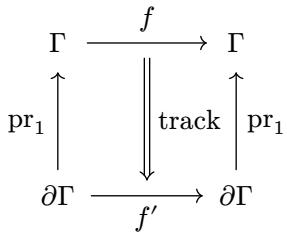
\includegraphics[keepaspectratio,alt={image}]{images/6ccf2193f4307249863af49c1bc005e170202baab7e50db5b126edc1426dfbe5.jpg}}

证明. 对所有 \(( \gamma , \varphi ) \in \partial \Gamma\)，

\[
\begin{array} { r }
  { ( \mathrm { p r } _ { 1 } \circ \mathrm { t r a c k } _ { \Gamma } ( f , g ) ) ( \gamma , \varphi ) = \mathrm { p r } _ { 1 } ( f ( \gamma ) , \varphi \circ g ) } \\
  { = f ( \gamma ) } \\
  { = ( f \circ \mathrm { p r } _ { 1 } ) ( \gamma , \varphi ) }
\end{array}
\]

定理 5. \(\operatorname { t r a c k } _ { \Gamma }\) 是从 \(\mathfrak { T } _ { \Gamma }\) 到
\(\partial \Gamma \to \partial \Gamma\) 的幺半群同态。即：

\begin{enumerate}
\def\labelenumi{\arabic{enumi}.}
\item
  \(\operatorname { t r a c k } _ { \Gamma } ( \mathrm { i d } _ { \Gamma } , \mathrm { i d } _ { \Gamma } ) = \mathrm { i d } _ { \partial \Gamma } ;\)
\item
  对所有
  \(( f _ { 1 } , g _ { 1 } ) , ( f _ { 2 } , g _ { 2 } ) \in \mathfrak { T } _ { \Gamma }\)，
\end{enumerate}

\[
\operatorname { t r a c k } _ { \Gamma } ( ( f _ { 1 } , g _ { 1 } ) \circ ( f _ { 2 } , g _ { 2 } ) ) = \operatorname { t r a c k } _ { \Gamma } ( f _ { 1 } , g _ { 1 } ) \circ \operatorname { t r a c k } _ { \Gamma } ( f _ { 2 } , g _ { 2 } )\tag{8}
\]

证明.

\begin{enumerate}
\def\labelenumi{\arabic{enumi}.}
\item
  单位元被映为单位元，因为
  \(\operatorname { t r a c k } _ { \Gamma } ( \mathrm { i d } _ { \Gamma } , \mathrm { i d } _ { \Gamma } ) ( \gamma , \varphi ) = ( \gamma , \varphi \circ \mathrm { i d } _ { \Gamma } ) = ( \gamma , \varphi )\)。
\item
  对乘法，取任意 \(( \gamma , \varphi ) \in \partial \Gamma\)。
\end{enumerate}

\[
\begin{array} { r l }
  & ( \operatorname { t r a c k } _ { \Gamma } ( f _ { 1 } , g _ { 1 } ) \circ \operatorname { t r a c k } _ { \Gamma } ( f _ { 2 } , g _ { 2 } ) ) ( \gamma , \varphi ) = \operatorname { t r a c k } _ { \Gamma } ( f _ { 1 } , g _ { 1 } ) ( f _ { 2 } ( \gamma ) , \varphi \circ g _ { 2 } ) \\
  & \qquad = ( f _ { 1 } ( f _ { 2 } ( \gamma ) ) , \varphi \circ g _ { 2 } \circ g _ { 1 } ) \\
  & \qquad = \operatorname { t r a c k } _ { \Gamma } ( f _ { 1 } \circ f _ { 2 } , g _ { 2 } \circ g _ { 1 } ) ( \gamma , \varphi )
\end{array}
\]

定义 6. 定义 \(\partial \Gamma\) 上的变换 \(\operatorname { r e c o v e r } _ { \Gamma }\)：

\[
\begin{array} { l r c l }
  { \operatorname { r e c o v e r } _ { \Gamma } } & { \colon } & { \partial \Gamma } & { \to \quad \partial \Gamma } \\
  { \operatorname { r e c o v e r } _ { \Gamma } } & { = } & { ( \gamma , \varphi ) } & { \mapsto ( \varphi ( \gamma ) , \mathrm { i d } _ { \Gamma } ) }
\end{array}\tag{9}
\]

该变换把恢复函数 \(\varphi\) 应用于当前状态 \(\gamma\)，并把 \(\varphi\) 重置为恒等函数。下图说明在效应序列
\(\operatorname { t r a c k } ( f _ { 1 } , g _ { 1 } ) , \cdots , \operatorname { t r a c k } ( f _ { n } , g _ { n } )\)
被应用于 \(\partial \Gamma\) 之后，recover 如何把上下文恢复到其初始状态：

\[
\begin{array} { r l }
  & \Gamma \xrightarrow { f _ { 1 } } \Gamma \longrightarrow \cdots \longrightarrow \Gamma \xrightarrow { f _ { n } } \Gamma \\
  & \Bigg \Updownarrow \mathrm { t r a c k } \qquad \qquad \qquad \qquad \Bigg \downarrow \mathrm { t r a c k } \\
  & \partial \Gamma \xrightarrow { f _ { 1 } ^ { \prime } } \partial \Gamma \longrightarrow \cdots \longrightarrow \partial \Gamma \xrightarrow { f _ { n } ^ { \prime } } \partial \Gamma \\
  & \Bigg \uparrow \qquad \qquad \qquad \qquad \qquad \mathrm { r e c o v e r }
\end{array}
\]

该图表明，被追踪的效应与随后的 recover 把初始效应上下文带回其自身。每一步追踪所保持的，正是从任意状态出发执行恢复所得的结果：

定理 7. 对任意 \(( \gamma , \varphi ) \in \partial \Gamma\) 以及满足
\(g ( f ( \gamma ) ) = \gamma\) 的任意对 \(( f , g )\)，

\[
\operatorname { r e c o v e r } _ { \Gamma } \bigl ( \operatorname { t r a c k } _ { \Gamma } ( f , g ) ( \gamma , \varphi ) \bigr ) = \operatorname { r e c o v e r } _ { \Gamma } ( \gamma , \varphi )\tag{10}
\]

证明.

\[
\begin{array} { r l }
  & \operatorname { r e c o v e r } _ { \Gamma } ( \operatorname { t r a c k } _ { \Gamma } ( f , g ) ( \gamma , \varphi ) ) = \operatorname { r e c o v e r } _ { \Gamma } ( f ( \gamma ) , \varphi \circ g ) \\
  & \qquad = ( \varphi ( g ( f ( \gamma ) ) ) , \mathrm { i d } _ { \Gamma } ) \\
  & \qquad = ( \varphi ( \gamma ) , \mathrm { i d } _ { \Gamma } ) = \operatorname { r e c o v e r } _ { \Gamma } ( \gamma , \varphi )
\end{array}
\]

对于成对的序列无需单独的论证。设 \(( f _ { 1 } , g _ { 1 } ) , \cdots , ( f _ { n } , g _ { n } )\) 从
\(( \gamma , \varphi )\) 出发按顺序施加，并记 \(\delta _ { 0 } = \gamma\) 与
\(\delta _ { i } : = f _ { i } ( \delta _ { i - 1 } )\)。由定理~5，复合追踪
\(\operatorname { t r a c k } _ { \Gamma } ( f _ { n } , g _ { n } ) \circ \cdots \circ \operatorname { t r a c k } _ { \Gamma } ( f _ { 1 } , g _ { 1 } )\)
正是扭曲复合
\(( f _ { n } \circ \cdots \circ f _ { 1 } , g _ { 1 } \circ \cdots \circ g _ { n } )\)
的追踪，并且若对每个 \(i\) 都有 \(g _ { i } ( \delta _ { i } ) = \delta _ { i - 1 }\)，则
\(( g _ { 1 } \circ \cdots \circ g _ { n } ) ( \delta _ { n } ) = \delta _ { 0 } = \gamma\)。
因此该对在 \(\gamma\) 处满足定理~7 的假设，应用一次该定理即得

\[
\operatorname { r e c o v e r } _ { \Gamma } ( ( \operatorname { t r a c k } _ { \Gamma } ( f _ { n } , g _ { n } ) \circ \dotsb \circ \operatorname { t r a c k } _ { \Gamma } ( f _ { 1 } , g _ { 1 } ) ) ( \gamma , \varphi ) ) = \operatorname { r e c o v e r } _ { \Gamma } ( \gamma , \varphi )\tag{11}
\]

取 \(( \gamma , \varphi ) = ( \gamma _ { 0 } , \mathrm { i d } _ { \Gamma } )\)，恢复会把按此方式到达的每个状态都带回
\(( \gamma _ { 0 } , \mathrm { i d } _ { \Gamma } )\)。满足 \(g \circ f = \operatorname { i d } _ { \Gamma }\) 的对在每个状态处都满足该假设。

恢复通过量 \(\varphi ( \gamma )\) 读取状态，我们把 \(\varphi ( \gamma ) = \gamma _ { 0 }\) 称为 \(\partial \Gamma\) 中状态的可靠性不变量。

\subsubsection{可逆效应函数} \label{revertible-efect-functions}

上一节的 track/recover 模型把逆变换视为先验给定的：\(\operatorname { t r a c k } _ { \Gamma } ( f , g )\) 在看到任何上下文状态之前就固定了 \(g\)，因此同一个 \(g\) 必须服务于效应施加处的每个状态。然而在实践中，每个效应的逆变换并非先验可知：它必须由调用者在效应施加点提供。此外，recover 是全有或全无的：它无法在保留其他效应的同时选择性地撤销某一个。为解决这两个问题，我们在输入侧与输出侧同时增强该模型：

\begin{enumerate}
\def\labelenumi{\arabic{enumi}.}
\item
  在输入侧，我们不仅变换 $\Gamma$，还随之返回一个逆变换函数，使得逆变换在效应施加处被提供：\(\Gamma \to \Gamma \times ( \Gamma \to \Gamma )\)，即
  \(\Gamma \to \partial \Gamma\)；
\item
  在输出侧，我们不仅变换 \(\partial \Gamma\)，还随之返回一个逆变换函数，使得一个效应可以在保留其他效应的同时被撤销：\(\partial \Gamma \to \partial \Gamma \times ( \partial \Gamma \to \partial \Gamma )\)，即
  \(\partial \Gamma \to \partial ^ { 2 } \Gamma\)。
\end{enumerate}

这种增强保持了输入与输出之间结构上的一致性，因此我们仍能定义相应的理论，以维持 track 的数学性质。由此得到的类型是效应函数 \(\mathfrak { E } _ { \Gamma }\) 及其带见证的精化版本
\({ \mathfrak { E } } _ { \Gamma } ^ { * }\)：

定义 8. 定义效应函数 \(\mathfrak { E } _ { \Gamma }\) 与见证效应函数
\({ \mathfrak { E } } _ { \Gamma } ^ { * }\)：

\[
\begin{array} { r l }
  & \mathfrak { E } _ { \Gamma } : = \Gamma \to \Gamma \times ( \Gamma \to \Gamma ) \\
  & \mathfrak { E } _ { \Gamma } ^ { * } : = \big ( e : \Gamma \to \Gamma \times ( \Gamma \to \Gamma ) \big ) \\
  & \quad \quad \times \big ( ( \gamma : \Gamma ) \to ( ( \delta : \Gamma ) \times ( g : \Gamma \to \Gamma ) \times ( ( \delta , g ) = e ( \gamma ) \to g ( \delta ) = \gamma ) ) \big )
\end{array}\tag{12}
\]

其中 \(e ( \gamma )\) 产生一个二元组 \(( \delta , g )\)，表示：

• \(\delta : \Gamma\) 是新的上下文；

• \(g : \Gamma \to \Gamma\) 是当前效应的逆变换函数。

\(\mathfrak { E } _ { \Gamma } ^ { * }\) 中的元素按状态选择其逆变换，约束 \(g ( \delta ) = \gamma\) 把该选择限定为在效应被施加处逆转效应，而在其他任何地方都不对 \(g\) 施加约束。满足
\(g \circ f = \operatorname { i d } _ { \Gamma }\) 的单个 \(g\) 同时满足每个状态处的约束，并通过
\(( f , g ) \mapsto \gamma \mapsto ( f ( \gamma ) , g )\) 诱导出 \(\mathfrak { E } _ { \Gamma } ^ { * }\) 中的一个元素，定理~11 将证明这是一个同态。该约束可以可视化为如下交换图，确保逆变换 \(g\) 确实在 \(e\) 被施加的状态处反转该变换：

\pandocbounded{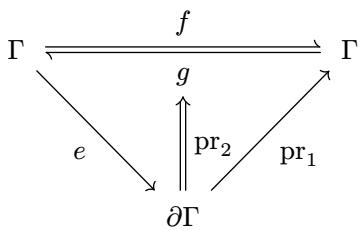
\includegraphics[keepaspectratio,alt={image}]{images/f2d6628215cd6fc08d01d2447a4d8728b73398e933b83424d748e2e755d79cc5.jpg}}

由于效应函数 \(\mathfrak { E } _ { \Gamma }\) 不再是上下文上的自同态，它们无法直接复合。因此我们为效应复合定义一个新的运算：

定义 9. 给定函数 \(f , g \in \mathfrak { E } _ { \Gamma }\)，定义它们的效应复合 \(f \diamond g\)：

\[
\begin{array} { l r c l }
  { f \diamond g } & { \colon } & { \Gamma } & { \to \partial \Gamma } \\
  { f \diamond g } & { = } & { \gamma } & { \mapsto \mathbf { l e t } \ ( \delta , s ) = g ( \gamma ) \ \mathbf { i n } \ \mathbf { l e t } \ ( \varepsilon , t ) = f ( \delta ) \ \mathbf { i n } \ ( \varepsilon , s \circ t ) }
\end{array}\tag{13}
\]

定理 10. 效应复合把 \(\mathfrak { T } _ { \Gamma }\) 的幺半群结构迁移到
\(\mathfrak { E } _ { \Gamma }\) 上。即：

\begin{enumerate}
\def\labelenumi{\arabic{enumi}.}
\item
  \(( \mathfrak { E } _ { \Gamma } , \diamond )\) 是幺半群，其单位元为
  \(\eta _ { \Gamma } : = \gamma \mapsto ( \gamma , \mathrm { i d } _ { \Gamma } ) ;\)
\item
  赋值 \(( f , g ) \mapsto \gamma \mapsto ( f ( \gamma ) , g )\) 是从 \(\mathfrak { T } _ { \Gamma }\) 到
  \(\mathfrak { E } _ { \Gamma }\) 的幺半群同态。
\end{enumerate}

证明.

\begin{enumerate}
\def\labelenumi{\arabic{enumi}.}
\item
  结合律与单位元定律按分量直接由 \(\circ\) 的相应性质得到。
\item
  记 \(e _ { i } = \gamma \mapsto ( f _ { i } ( \gamma ) , g _ { i } )\)；则
  \(( e _ { 1 } \diamond e _ { 2 } ) ( \gamma ) = ( f _ { 1 } ( f _ { 2 } ( \gamma ) ) , g _ { 2 } \circ g _ { 1 } )\)，
  即 \(\left( f _ { 1 } , g _ { 1 } \right) \circ \left( f _ { 2 } , g _ { 2 } \right)\) 的像，且
  \(( \mathrm { i d } _ { \Gamma } , \mathrm { i d } _ { \Gamma } )\) 映到 \(\eta _ { \Gamma }\)。□
\end{enumerate}

定理 11. 见证在效应复合下保持不变，且一致逆变换在每个状态处都构成见证。即：

\begin{enumerate}
\def\labelenumi{\arabic{enumi}.}
\item
  \(\mathfrak { E } _ { \Gamma } ^ { * }\) 是 \(\mathfrak { E } _ { \Gamma }\) 的子幺半群；
\item
  定理~10 中的同态把每个满足 \(g \circ f = \operatorname { i d } _ { \Gamma }\) 的对都映入
  \(\mathfrak { E } _ { \Gamma } ^ { * }\)。
\end{enumerate}

证明.

\begin{enumerate}
\def\labelenumi{\arabic{enumi}.}
\item
  单位元位于 \(\mathfrak { E } _ { \Gamma } ^ { * }\) 中，因为
  \(\operatorname { i d } _ { \Gamma } ( \gamma ) = \gamma\)。对封闭性，取
  \(f , g \in \mathfrak { E } _ { \Gamma } ^ { * }\) 及任意 \(\gamma \in \Gamma\)，设
  \(( \delta , s ) = g ( \gamma )\)、\(( \varepsilon , t ) = f ( \delta )\)，于是
  \(( f \diamond g ) ( \gamma ) = ( \varepsilon , s \circ t )\)。那么
  \(s ( \delta ) = \gamma\) 且 \(t ( \varepsilon ) = \delta\)，从而
  \(( s \circ t ) ( \varepsilon ) = s ( \delta ) = \gamma\)。
\item
  \(g \circ f = \operatorname { i d } _ { \Gamma }\) 给出对每个 \(\gamma\) 有
  \(g ( f ( \gamma ) ) = \gamma\)，因此这类对的像在每个状态处都被见证。□
\end{enumerate}

正如 track 把 $\Gamma$ 上的一对变换提升到 \(\partial \Gamma\)，我们定义 effect 把
\(\mathfrak { E } _ { \Gamma }\) 提升到 \(\mathfrak { E } _ { \partial \Gamma }\)：

定义 12. 定义效应函数变换 \(\operatorname { e f f e c t } _ { \Gamma }\)：

\[
\begin{array} { l r c l c l }
  { \operatorname { e f f e c t } _ { \Gamma } } & { \colon } & { \mathfrak { E } _ { \Gamma } } & { \to } & { \partial \Gamma } & { \to \partial ^ { 2 } \Gamma } \\
  { \operatorname { e f f e c t } _ { \Gamma } } & { = } & { e } & { \mapsto } & { ( \gamma , \varphi ) } & { \mapsto \mathbf { l e t } \ ( \delta , g ) = e ( \gamma ) \ \mathbf { i n } \ ( ( \delta , \varphi \circ g ) , \operatorname { t r a c k } _ { \Gamma } ( g , \operatorname { p r } _ { 1 } \circ e ) ) }
\end{array}\tag{14}
\]

由于 \(\operatorname { e f f e c t } _ { \Gamma } ( e )\) 本身是 \(\mathfrak { E } _ { \partial \Gamma }\) 中的元素，它所返回的逆变换应按定义~8 高一层的意义来理解。该逆变换本身正是交换效应的两个方向所得之对的一个追踪。普通的追踪规则再次适用：撤销效应本身也是一个效应，它以 \(g\) 变换状态，而撤销它的方式就是再次执行该效应，这正是 \(\operatorname { p r } _ { 1 } \circ e\) 所做的。因此该逆变换复合到交给它的累加器上，恰如 track 所规定的那样。

我们现在可以证明 effect 与 track 相类似的性质。

定理 13. effect 保持 $\diamond$ 运算。即，对所有 \(f , g \in \mathfrak { E } _ { \Gamma }\)，

\[
\operatorname { e f f e c t } _ { \Gamma } ( f ) \diamond \operatorname { e f f e c t } _ { \Gamma } ( g ) = \operatorname { e f f e c t } _ { \Gamma } ( f \diamond g )\tag{15}
\]

证明. 取任意 \(( \gamma , \varphi ) \in \partial \Gamma\)，设
\(( \delta , s ) = g ( \gamma )\) 与 \(( \varepsilon , t ) = f ( \delta )\)，于是
\(( f \diamond g ) ( \gamma ) = ( \varepsilon , s \circ t )\)，且
\(\operatorname { p r } _ { 1 } \circ ( f \diamond g ) = ( \operatorname { p r } _ { 1 } \circ f ) \circ ( \operatorname { p r } _ { 1 } \circ g )\)。则

\[
\begin{array} { r l }
  & ( \operatorname { e f f e c t } _ { \Gamma } ( f ) \diamond \operatorname { e f f e c t } _ { \Gamma } ( g ) ) ( \gamma , \varphi ) = ( ( \varepsilon , \varphi \circ s \circ t ) , \operatorname { t r a c k } _ { \Gamma } ( s , \operatorname { p r } _ { 1 } \circ g ) \circ \operatorname { t r a c k } _ { \Gamma } ( t , \operatorname { p r } _ { 1 } \circ f ) ) \\
  & \qquad = ( ( \varepsilon , \varphi \circ s \circ t ) , \operatorname { t r a c k } _ { \Gamma } ( s \circ t , ( \operatorname { p r } _ { 1 } \circ f ) \circ ( \operatorname { p r } _ { 1 } \circ g ) ) ) \\
  & \qquad = \operatorname { e f f e c t } _ { \Gamma } ( f \diamond g ) ( \gamma , \varphi )
\end{array}
\]

其中第一步在 \(( \gamma , \varphi )\) 与 \(( \delta , \varphi \circ s )\) 处展开定义~12，第二步用到定理~5，第三步折叠定义~12。□

两个层次之间的关系由下图展示。其上三角是 \(e\) 的见证条件（按定义~8），其下三角则是
\(e ^ { \prime }\) 是否像 \(e\) 一样被见证的问题。

\pandocbounded{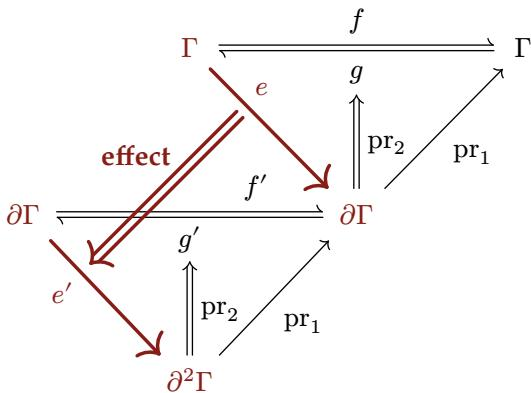
\includegraphics[keepaspectratio,alt={image}]{images/21186ec878faabc31d96dd91c90577b582af7acf8a5b61cde0f72d038f47fa16.jpg}}

在层次之间，投影 \(\operatorname { p r } _ { 1 }\) 把每个被提升的映射与其所提升的映射联系起来，正如它在定理~4 中为 track 所做的那样。

定理 14. 设 \(e \in \mathfrak { E } _ { \Gamma }\)，记 \(f : = \operatorname { p r } _ { 1 } \circ e\)，并令
\(e ^ { \prime } : = \operatorname { e f f e c t } _ { \Gamma } ( e )\)，其前向映射为
\(f ^ { \prime } : = \operatorname { p r } _ { 1 } \circ e ^ { \prime }\)。则

\begin{enumerate}
\def\labelenumi{\arabic{enumi}.}
\item
  \(\operatorname { p r } _ { 1 } \circ f ^ { \prime } = f \circ \operatorname { p r } _ { 1 } ;\)
\item
  对每个 \(( \gamma , \varphi ) \in \partial \Gamma\)，在该处被见证的提升逆变换
  \(g ^ { \prime } : = \operatorname { p r } _ { 2 } ( e ^ { \prime } ( \gamma , \varphi ) )\) 与逆变换
  \(g : = \operatorname { p r } _ { 2 } ( e ( \gamma ) )\) 满足
  \(\operatorname { p r } _ { 1 } \circ g ^ { \prime } = g \circ \operatorname { p r } _ { 1 }\)。
\end{enumerate}

证明.

\begin{enumerate}
\def\labelenumi{\arabic{enumi}.}
\item
  由定义~12，
  \(f ^ { \prime } ( \gamma , \varphi ) = ( f ( \gamma ) , \varphi \circ g )\)，
  其状态为
  \(f ( \gamma ) = ( f \circ \operatorname { p r } _ { 1 } ) ( \gamma , \varphi )\)。
\item
  这是对 \(g ^ { \prime } = \operatorname { t r a c k } _ { \Gamma } ( g , f )\) 应用定理~4。
\end{enumerate}

下三角是否闭合，可通过计算被提升的逆变换所返回的内容来确定：

定理 15. 设 \(e \in \mathfrak { E } _ { \Gamma } ^ { * }\)，记 \(f : = \operatorname { p r } _ { 1 } \circ e\)。固定
\(( \gamma , \varphi ) \in \partial \Gamma\)，设 \(( \delta , g ) = e ( \gamma )\)，并以
\(( \Delta , g ^ { \prime } )\) 表示 \(\operatorname { e f f e c t } _ { \Gamma } ( e )\) 在
\(( \gamma , \varphi )\) 处的值。则

\[
g ^ { \prime } ( \Delta ) = ( \gamma , \varphi \circ g \circ f )\tag{16}
\]

状态被精确恢复。累加器也被恢复——等价地，
\(\operatorname { e f f e c t } _ { \Gamma } ( e ) \in \mathfrak { E } _ { \partial \Gamma } ^ { * }\)——当且仅当
\(g \circ f = \operatorname { i d } _ { \Gamma }\)；并且在任何情况下都有
\(( \varphi \circ g \circ f ) ( \gamma ) = \varphi ( \gamma )\)，因此可靠性不变量得以保持。

证明. 由定义~12，\(\Delta = ( \delta , \varphi \circ g )\) 且
\(g ^ { \prime } = \operatorname { t r a c k } _ { \Gamma } ( g , f )\)，所以

\[
g ^ { \prime } ( \Delta ) = ( g ( \delta ) , \varphi \circ g \circ f ) = ( \gamma , \varphi \circ g \circ f )
\]

其中用到了 \(g ( \delta ) = \gamma\)。要属于 \(\mathfrak { E } _ { \partial \Gamma } ^ { * }\)，需对每个输入都等于
\(( \gamma , \varphi )\)；取 \(\varphi = \mathrm { i d } _ { \Gamma }\) 可把累加器的相等化为
\(g \circ f = \operatorname { i d } _ { \Gamma }\)，而该条件反过来又对每个 \(\varphi\) 给出累加器的相等。最后，
\(( \varphi \circ g \circ f ) ( \gamma ) = \varphi ( g ( \delta ) ) = \varphi ( \gamma )\)。□

因此，只有当在 \(\gamma\) 处被见证的逆变换在每个状态处都逆转 \(f\) 时，下三角才会闭合，所以
\(\operatorname { e f f e c t } _ { \Gamma }\) 不把 \(\mathfrak { E } _ { \Gamma } ^ { * }\) 映入
\(\mathfrak { E } _ { \partial \Gamma } ^ { * }\)。在任何情况下都成立的是在 \(\gamma\) 处的一致：
\(\operatorname { r e c o v e r } _ { \Gamma } ( g ^ { \prime } ( \Delta ) ) = \operatorname { r e c o v e r } _ { \Gamma } ( \gamma , \varphi )\)，这正是定理~7 对累加器所假设的全部内容，因此逆转不会触及恢复目标。

按施加顺序之逆序逆转效应无需任何额外条件，因为此时每个逆变换面对的正是其自身施加所产生的那个状态：

定理 16. 设 \(e _ { 1 } , \cdots , e _ { n } \in \mathfrak { E } _ { \Gamma } ^ { * }\) 从
\(( \gamma _ { 0 } , \mathrm { i d } _ { \Gamma } )\) 出发按顺序施加并按逆序逆转。则

\begin{enumerate}
\def\labelenumi{\arabic{enumi}.}
\item
  每次逆转都恢复其施加时所针对的上下文状态；
\item
  每个中间状态都满足可靠性不变量。
\end{enumerate}

证明. 每一步要么是一次施加，要么是一次逆转。一次施加把 \(( \gamma , \varphi )\) 带到
\(( \delta , \varphi \circ g )\)，其中 \(g ( \delta ) = \gamma\)，因此由定理~7 它保持
\(\varphi ( \gamma )\)，而定理~7 的假设正是 \(\mathfrak { E } _ { \Gamma } ^ { * }\) 的见证。按逆序逆转使每个逆变换面对其自身施加所产生的状态，因此由定理~15，该次逆转精确恢复前一个状态，并同样保持
\(\varphi ( \gamma )\)；这两个结论都不依赖于逆变换所接收到的累加器。□

\subsubsection{效应的独立性} \label{independence-of-efects}

在效应自身施加所产生的状态下逆转它，是定理~16 所覆盖的情形；在其他任何状态下逆转它，则是本小节覆盖的情形。有两种情况需要后者。一种情况是逆变换在更晚的效应仍然在位时运行，这正相当于从运行中的系统中撤回一个组件；另一种情况是一个序列可以交错多个组件的效应，每个组件各自保留自己的逆变换，因此一个组件的逆变换被另一个组件的施加所分隔。在这两种情况下，逆变换所面对的状态都被外来效应移动过，而它是否仍能逆转它原本要逆转的内容，是一个交换性问题：需要交换的是，一个效应所能执行的每个变换与另一个效应所能执行的每个变换，前向映射与所产出的逆变换都一样。单独的累加器无法解决这两种情形，因为 \(\varphi\) 是一个复合，它以单一顺序一次性运行它所持有的每个逆变换。

定义 17. 对效应函数 \(e \in \mathfrak { E } _ { \Gamma }\)，变换幺半群
\(\mathfrak { M } ( e )\) 是由 \(e\) 的前向映射连同 \(e\) 产出的每个逆变换生成的
\(\Gamma \to \Gamma\) 的子幺半群，而 \(\mathfrak { M } ( e )\) 的生成元就是该生成集的元素：

\[
\mathfrak { M } ( e ) : = \langle \{ \mathrm { p r } _ { 1 } \circ e \} \cup \{ \mathrm { p r } _ { 2 } ( e ( \gamma ) ) \mid \gamma \in \Gamma \} \rangle\tag{17}
\]

由对 \(( f , g ) \in \mathfrak { T } _ { \Gamma }\) 诱导的效应以 \(f\) 与 \(g\) 为生成元，它在每个状态处产出的逆变换都是 \(g\)。

引理 18. 交换性在生成元上即可判定，且 $\diamond$ 不扩大任何变换幺半群。即：

\begin{enumerate}
\def\labelenumi{\arabic{enumi}.}
\item
  若 \(\mathfrak { M } ( e _ { 1 } )\) 的每个生成元都与 \(\mathfrak { M } ( e _ { 2 } )\) 的每个生成元交换，则
  \(\mathfrak { M } ( e _ { 1 } )\) 的每个元素都与 \(\mathfrak { M } ( e _ { 2 } )\) 的每个元素交换；
\item
  \(\mathfrak { M } ( e _ { 1 } \diamond e _ { 2 } ) \subseteq \langle \mathfrak { M } ( e _ { 1 } ) \cup \mathfrak { M } ( e _ { 2 } ) \rangle\)。
\end{enumerate}

证明.

\begin{enumerate}
\def\labelenumi{\arabic{enumi}.}
\item
  与 \(\mathfrak { M } ( e _ { 2 } )\) 的每个生成元交换的映射构成 \(\Gamma \to \Gamma\) 的一个子幺半群，因为
  \(\mathrm { i d } _ { \Gamma }\) 位于其中，且当 \(f\) 与 \(f ^ { \prime }\) 都在其中时
  \(f \circ f ^ { \prime }\) 也在其中。该子幺半群按假设包含 \(\mathfrak { M } ( e _ { 1 } )\) 的生成元，因而包含
  \(\mathfrak { M } ( e _ { 1 } )\)。固定 \(f \in \mathfrak { M } ( e _ { 1 } )\)，与 \(f\) 交换的映射同样构成一个子幺半群，它包含 \(\mathfrak { M } ( e _ { 2 } )\) 的生成元，因而包含
  \(\mathfrak { M } ( e _ { 2 } )\)。
\item
  由定义~9，\(e _ { 1 } \diamond e _ { 2 }\) 的前向映射是
  \(\left( \mathrm { p r } _ { 1 } \circ e _ { 1 } \right) \circ \left( \mathrm { p r } _ { 1 } \circ e _ { 2 } \right)\)，且它在任何状态处产出的逆变换都是 \(s \circ t\)，其中 \(s\) 由 \(e _ { 2 }\) 产出、\(t\) 由 \(e _ { 1 }\) 产出。因此
  \(\mathfrak { M } ( e _ { 1 } \diamond e _ { 2 } )\) 的每个生成元都是二者生成元的复合。□
\end{enumerate}

定义 19. 效应函数 \(e _ { 1 } , e _ { 2 } \in \mathfrak { E } _ { \Gamma }\) 当且仅当以下条件成立时称为独立的：

\begin{enumerate}
\def\labelenumi{\arabic{enumi}.}
\tightlist
\item
  其中一方的每个变换都与另一方的每个变换交换，
\end{enumerate}

\[
\forall f \in \mathfrak { M } ( e _ { 1 } ) , g \in \mathfrak { M } ( e _ { 2 } ) . \quad f \circ g = g \circ f\tag{18}
\]

\begin{enumerate}
\def\labelenumi{\arabic{enumi}.}
\setcounter{enumi}{1}
\tightlist
\item
  其中一方的变换都不扰动另一方所产出的逆变换，
\end{enumerate}

\[
\forall g \in \mathfrak { M } ( e _ { 2 } ) , \gamma \in \Gamma . \quad \mathrm { p r } _ { 2 } ( e _ { 1 } ( g ( \gamma ) ) ) = \mathrm { p r } _ { 2 } ( e _ { 1 } ( \gamma ) )\tag{19}
\]

并且交换 \(e _ { 1 }\) 与 \(e _ { 2 }\) 后同样成立。

族 \(\left( e _ { l } \right) _ { l \in L }\) 两两独立，是指对每个 \(l \neq l ^ { \prime }\)，\(e _ { l }\) 与
\(e _ { l ^ { \prime } }\) 都独立。一个族可以重复同一个效应函数，而使一个效应与自身独立，就是要使
\(\mathfrak { M } ( e )\) 交换。

对于由对 \(( f _ { 1 } , g _ { 1 } )\) 与 \(( f _ { 2 } , g _ { 2 } )\) 诱导的效应，条件 (1) 由引理~18(1) 等价于四对
\(f _ { 1 } , f _ { 2 }\)；\(g _ { 1 } , g _ { 2 }\)；\(f _ { 1 } , g _ { 2 }\)；与 \(g _ { 1 } , f _ { 2 }\) 的交换，而条件 (2) 直接成立，因为诱导效应在每个状态处只产出一个逆变换。在 $\diamond$ 下的交换是一个不同的性质。\(e _ { 1 } \diamond e _ { 2 } = e _ { 2 } \diamond e _ { 1 }\) 所等同的是：两种顺序下复合前向映射彼此相等，两种顺序下复合逆变换彼此相等，其中每个逆变换都在其自身施加所产生的状态处进入复合；独立性则把一方的每个变换与另一方的每个变换对应起来，包括前向映射与外来逆变换的配对。

在独立性下，逆变换可以在被更晚的效应移动过的状态处运行，而它在彼处撤回的只是自身的贡献，别无其他：

定理 20. 设 \(e _ { 1 } , \cdots , e _ { n } \in \mathfrak { E } _ { \Gamma } ^ { * }\) 两两独立，并从
\(\gamma _ { 0 }\) 出发按顺序施加。记 \(f _ { i } : = \mathbf { p r } _ { 1 } \circ e _ { i }\)，令
\(\delta _ { i } : = f _ { i } ( \delta _ { i - 1 } )\) 且 \(\delta _ { 0 } : = \gamma _ { 0 }\)，并令
\(g _ { i } : = \mathrm { p r } _ { 2 } ( e _ { i } ( \delta _ { i - 1 } ) )\) 为 \(e _ { i }\) 在施加处产出的逆变换。固定
\(j\)，记 \(\delta _ { i } ^ { \prime } : = \big ( f _ { i } \circ \cdots \circ f _ { j + 1 } \big ) \big ( \delta _ { j - 1 } \big )\) 为剔除 \(e _ { j }\) 后该序列的各状态，于是
\(\delta _ { j } ^ { \prime } = \delta _ { j - 1 }\)。则对每个满足 \(j \leq u \leq n\) 的 \(u\)：

\begin{enumerate}
\def\labelenumi{\arabic{enumi}.}
\item
  \(\delta _ { u } = f _ { j } ( \delta _ { u } ^ { \prime } )\) 且
  \(g _ { j } ( \delta _ { u } ) = \delta _ { u } ^ { \prime }\)；
\item
  每个满足 \(i > j\) 的 \(e _ { i }\) 在 \(\delta _ { i - 1 } ^ { \prime }\) 处产出的逆变换，与它在
  \(\delta _ { i - 1 }\) 处产出的逆变换相同，即 \(g _ { i }\)。
\end{enumerate}

证明.

\begin{enumerate}
\def\labelenumi{\arabic{enumi}.}
\tightlist
\item
  第一个等式是对 \(u\) 的归纳。在 \(u = j\) 处它读作
  \(\delta _ { j } = f _ { j } \big ( \delta _ { j - 1 } \big )\)，即 \(\delta _ { j }\) 的定义。对归纳步，
  \(\delta _ { u + 1 } = f _ { u + 1 } ( \delta _ { u } ) = f _ { u + 1 } ( f _ { j } ( \delta _ { u } ^ { \prime } ) ) = f _ { j } ( f _ { u + 1 } ( \delta _ { u } ^ { \prime } ) ) = f _ { j } \left( \delta _ { u + 1 } ^ { \prime } \right)\)，
  中间的等式用到定义~19 的条件 (1)，对 \(e _ { u + 1 }\) 与 \(e _ { j }\)，它们是该族中互异的效应，因为 \(u + 1 > j\)。对第二个等式，条件 (1) 把 \(g _ { j }\) 穿过在 \(e _ { j }\) 之后施加的前向映射带出来，把 \(e _ { j }\) 的见证留在它成立的那一个状态处使用：
\end{enumerate}

\[
g _ { j } ( \delta _ { u } ) = \bigl ( g _ { j } \circ f _ { u } \circ \cdots \circ f _ { j + 1 } \bigr ) \bigl ( \delta _ { j } \bigr ) = \bigl ( f _ { u } \circ \cdots \circ f _ { j + 1 } \bigr ) \bigl ( g _ { j } \bigl ( f _ { j } \bigl ( \delta _ { j - 1 } \bigr ) \bigr ) \bigr ) = \delta _ { u } ^ { \prime }
\]

最后一个等式依赖于
\(g _ { j } \big ( f _ { j } \big ( \delta _ { j - 1 } \big ) \big ) = \delta _ { j - 1 }\)，这是定义~8 要求 \(e _ { j }\) 在
\(\delta _ { j - 1 }\) 处满足的见证。

\begin{enumerate}
\def\labelenumi{\arabic{enumi}.}
\setcounter{enumi}{1}
\tightlist
\item
  由 (1)，状态 \(\delta _ { i - 1 }\) 是 \(f _ { j } ( \delta _ { i - 1 } ^ { \prime } )\)，且
  \(f _ { j } \in \mathfrak { M } ( e _ { j } )\)，因此对 \(e _ { i }\) 与 \(e _ { j }\) 应用定义~19 的条件 (2) 给出
  \(\mathrm { p r } _ { 2 } \big ( e _ { i } \big ( f _ { j } ( \delta _ { i - 1 } ^ { \prime } ) \big ) \big ) = \mathrm { p r } _ { 2 } \big ( e _ { i } ( \delta _ { i - 1 } ^ { \prime } ) \big )\)。□
\end{enumerate}

条件 (1) 定位了逆变换所到达的状态：即同一序列在该效应从未被施加的情况下本会到达的状态，无论其后施加了什么效应。条件 (2) 定位了其他效应在那里所持有的逆变换，二者合起来使该定理可以再次应用于更短的序列：

推论 21. 设 \(e _ { 1 } , \cdots , e _ { n } \in \mathfrak { E } _ { \Gamma } ^ { * }\) 两两独立，从
\(\gamma _ { 0 }\) 出发按顺序施加，并令 \(g _ { 1 } , \cdots , g _ { n }\) 如上。在 \(\delta _ { n }\) 处按
\(\{ 1 , \cdots , n \}\) 的任意排列的顺序施加这 \(n\) 个逆变换，都会到达 \(\gamma _ { 0 }\)。

证明. 对 \(n\) 向下归纳。设该排列以 \(j\) 开头。由定理~20(1)，在 \(\delta _ { n }\) 处施加 \(g _ { j }\) 到达
\(\delta _ { n } ^ { \prime }\)，即剔除 \(e _ { j }\) 后该序列所到达的状态，而由定理~20(2)，其余效应在那里产出的逆变换正是手中的 \(g _ { i }\)。该序列两两独立，因为它是子族，所以归纳假设适用于它以及排列的其余部分；空序列到达
\(\gamma _ { 0 }\)。□

LIFO 顺序正是这样一个排列，定理~16 在其中无需任何假设即可逆转。独立性带来的则是所有其他顺序，以及随之而来的交错多个组件的序列，第 4.4.2 节将其推广到整个系统的迹。

综上，这些构造共同构成可逆效应：\(\mathfrak { E } _ { \Gamma } ^ { * }\) 中的每个效应函数都显式地提供自身的逆变换，effect 在效应上下文 \(\partial \Gamma\) 上追踪这些逆变换，而 $\diamond$ 运算在保持可逆性的同时将它们复合。它们所带来的是局部的时序可组合性；所谓局部，是指该保证只针对单一组件的效应本身来解读。我们把它理解为如下准则：对于组件施加的每一个效应函数序列，累加器都恢复它所出发的上下文（定理~7），而逆转该序列时每个逆变换面对的正是其自身施加时所针对的状态（定理~16）。加载一个组件就是施加这样一个序列并把它的逆变换累积到 \(\varphi\) 中；卸载它就是施加 \(\varphi\)。

准则遗漏了两件事，而这两件事都在多个组件参与时才出现：脱离累加器所强加顺序的逆转，以及交错他人效应的序列。独立性提供了它们（推论~21），它是关于效应本身的一个条件，而非构造的性质；第 3.3.2 节识别了满足该条件的纪律，第 4.4.2 节则从整个系统的迹的角度解读该保证。当独立性不成立时，顺序必须由其他机制承担：在单一组件内部由累加器承担，无论效应为何，它都按 LIFO 顺序逆转（第 4.3.2 节）；跨组件则由声明式的余效应承担，它让一次激活对另一次激活排序（第 4.3.1 节）。
\subsection{响应式余效应} \label{reactive-coefects}

空间可组合性是指组件之间能够相互声明依赖，系统能够在运行时解析、供给和撤回这些依赖的能力。这要求在共享上下文每次变化时都重新评估依赖满足状况，使组件在依赖变为可用时激活、在依赖被撤回时停用。因此，我们把组件的依赖建模为一种规格，并对照该规格把每一次上下文变更分类为激活性的、停用性的或中性的。对照规格进行分类，正是检测满足状况变化的手段；对分类作出响应，则是驱动激活与停用的机制。我们把这样的余效应称为响应式：通过分类上下文变更并据此驱动激活与停用，正确的余效应排序便成为结构性的保证。

\subsubsection{余效应上下文} \label{coefect-context}

传统的控制反转（inversion-of-control，IoC）容器 {[}38{]} 通常把依赖建模为简单的键值映射。本节把 IoC 形式化为一种余效应上下文，它与可逆效应协同工作，为动态组合提供数学基础。

定义 22. 给定类型族 \(\mathcal { V } : K \to \mathrm { T y p e }\)，把余效应上下文定义为依值部分函数类型：

\[
\Sigma : = ( k : K ) \rightharpoonup \mathcal { V } _ { k }\tag{20}
\]

其中 \(\sigma : \Sigma\) 是一个有限部分函数，为每个 \(k \in \mathrm { d o m } ( \sigma ) \subseteq K\) 赋一个类型 \(\mathcal { V } _ { k }\) 的值。我们记：

\begin{itemize}
\item \(\sigma ( k )\) 表示应用（当 \(k \in \mathrm { d o m } ( \sigma )\) 时有定义）；
\item \(\sigma [ k \mapsto v ]\) 表示表绑定：在 \(k\) 处绑定 \(v\)，在其余各处与 \(\sigma\) 一致；
\item \(\sigma \setminus k\) 表示限制（当 \(k \in \mathrm { d o m } ( \sigma )\) 时有定义）；
\item \(k \in \mathrm { d o m } ( \sigma )\) 表示成员关系。
\end{itemize}

使用类型族 \(\mathcal { V }\) 保证了每个依赖键 \(k\) 都与一个特定的值类型 \(\mathcal { V } _ { k }\) 相关联，为依赖访问提供静态类型安全。扩展与限制带有前置条件，由下面的运算强加：一个依赖不能被供给两次（扩展要求 \(k \notin \mathrm { d o m } ( \sigma )\)），也不能在不存在时被撤销（限制要求 \(k \in \mathrm { d o m } ( \sigma )\)）。违反前置条件会被报告为错误且不产生任何转移，因此描述实际所发生转移的效应代数可原样应用于这些运算。更倾向于把失败内化的读者，可以把下文中的每个 \(\Sigma \rightharpoonup \Sigma\) 读作 \(\Sigma \to \mathsf { Maybe } ( \Sigma )\)，并在 \(\mathsf { Maybe }\) 单子（第~2.1 节）中组合，代价是把每个恒等替换为运算定义域上的部分恒等。基于这一上下文结构，我们定义两个核心运算：

定义 23. \(\Sigma\) 上的 get 与 set 运算定义如下：

\[
\begin{array} { r c c c c c c } { \mathrm { g e t } } & { : } & { ( k : K ) } & { \to } & { \Sigma } & { \rightharpoonup } & { \mathcal { V } _ { k } } \\ { \mathrm { g e t } } & { = } & { k } & { \mapsto } & { \sigma } & { \mapsto } & { \sigma ( k ) } \\ { \mathrm { s e t } } & { : } & { ( k : K ) \times \mathcal { V } _ { k } } & { \to } & { \Sigma } & { \rightharpoonup } & { \Sigma \times ( \Sigma \rightharpoonup \Sigma ) } \\ { \mathrm { s e t } } & { = } & { ( k , v ) } & { \mapsto } & { \sigma } & { \mapsto } & { ( \sigma [ k \mapsto v ] , \lambda \sigma ^ { \prime } . \sigma ^ { \prime } \setminus k ) } \end{array}\tag{21}
\]

其中 get\(( k )\) 以 \(k \in \mathrm { d o m } ( \sigma )\) 为前置条件，set\(( k , v )\) 以 \(k \notin \mathrm { d o m } ( \sigma )\) 为前置条件。

值得注意的是，set\(( k , v )\) 具有类型 \(\mathfrak { E } _ { \Sigma } ^ { * }\)，正是一个余效应上下文上的效应函数。因此我们可以直接应用第~3.1 节的效应机制：effect\(\Sigma\) 提供依赖注册的自动追踪与恢复。这正是响应式余效应与可逆效应之间的协同：余效应运算就是效应，而效应是可逆的。

get 交给组件的是一个值，而组件能用这个值做什么，取决于该键处的余效应提供了什么。因此，一个键承载的不仅仅是值类型：

定义 24. 键 \(k\) 处的余效应是一个三元组 \(\left( \mathcal { V } _ { k } , \simeq _ { k } , \mathcal { A } _ { k } \right)\)，其中 \(\mathcal { V } _ { k }\) 是定义~22 的值类型，\(\simeq _ { k }\) 是 \(\mathcal { V } _ { k }\) 上的一个等价关系，\(k\) 处的值按该关系进行比较（第~3.3.2 节），\(\mathcal { A } _ { k }\) 是一组余效应运算，即绑定在 \(k\) 处的值向持有它的组件提供的那些运算。一个运算 \(a \in \mathcal { A } _ { k }\) 带有一个参数类型 \(X _ { a }\) 和一个结果类型 \(B _ { a }\)，并且只作用于该值本身：

\[
a : X _ { a } \to \mathcal { V } _ { k } \rightharpoonup \mathcal { V } _ { k } \times ( \mathcal { V } _ { k } \rightharpoonup \mathcal { V } _ { k } ) \times B _ { a }\tag{22}
\]

其前两个分量构成 \(\mathcal { V } _ { k }\) 上的一个效应函数，正如定义~8 所要求的那样被见证；第三个分量则是结果。每个运算都要求尊重 \(\simeq _ { k }\)：在 \(\simeq _ { k }\) 相关的值上，它要么在两者上都有定义，要么在两者上都无定义；在有定义处，它产生 \(\simeq _ { k }\) 相关的后继，其逆再次把 \(\simeq _ { k }\) 相关的值带到 \(\simeq _ { k }\) 相关的值，并产生相同的结果。一个运算通过它的 lift 作用于余效应上下文：

\[
a ^ { \Sigma } ( x ) ( \sigma ) : = \mathrm { { l e t } } \ ( v , g , b ) = a ( x ) ( \sigma ( k ) ) \mathrm { { i n } } \ ( \sigma [ k \mapsto v ] , \lambda \sigma ^ { \prime } . \sigma ^ { \prime } [ k \mapsto g ( \sigma ^ { \prime } ( k ) ) ] , b )\tag{23}
\]

当 \(k \in \mathrm { d o m } ( \sigma )\) 时有定义，其前两个分量是 \(\Sigma\) 上的一个效应函数。

把键 \(k\) 的运算类型化为作用在 \(\mathcal { V } _ { k }\) 上，正是将其约束在 \(k\) 处的绑定上：该 lift 读取并写入这个绑定，而让其他所有键保持原样，因此无需附加条件即可表达这一点。在隔离生效之处，它到达的绑定正是领域解析到的那个绑定（定义~28），共享同一领域的两个键共享同一个绑定。行为取决于其他键的运算，会把这个键的值读入其参数 \(X _ { a }\)，而下一小节的响应式纪律保证：只要读取了该值的组件仍在运行，该值就保持不变（定理~63）。

\subsubsection{规格与通知} \label{specification-and-notification}

前面的定义描述了单个依赖如何被注册和访问。然而，访问一个不存在的依赖是运行时错误。因此，组件应当只在它声明的所有依赖都就绪之后才激活，而不是乐观地访问它们、在某个依赖缺失时失败。这引出两个问题：组件的声明依赖是否被共同满足，以及当这一状态变化时系统应如何响应。余效应上下文 \(\Sigma\) 具有一种自然的可观察结构，使这两个问题都可处理：对任意余效应规格 \(d \subseteq K\)，定义满足谓词：

\[
\sigma \models d : = \forall k \in d . k \in \operatorname { d o m } ( \sigma )\tag{24}
\]

该谓词是可判定的（因为 dom\(( \sigma )\) 是有限的）。由于对 \(\sigma\) 的所有变更都经由效应函数（其逆恢复先前的定义域），满足状况的变化在每个效应边界上都是可检测的。这就是响应性的代数基础：效应系统保证每一次余效应变更都会被观察到。

定义 25. 余效应规格是：

\[
{ \mathfrak { D } } _ { \Sigma } : = { \mathsf { S e t } } ( K )\tag{25}
\]

它表示一个组件从环境中声明的依赖集合。

使这种规格具有响应性的，是它如何对状态转移进行分类。任何把 \(\sigma\) 变换为 \(\sigma ^ { \prime }\) 的效应，都可以由规格 \(d \in \mathfrak { D } _ { \Sigma }\) 根据 \(d\) 的满足状况是否被改变来分类：

定义 26. 给定余效应规格 \(d \subseteq K\) 和状态 \(\sigma , \sigma ^ { \prime } \in \Sigma\)，定义：

\[
\mathrm { n o t i f y } _ { d } ( \sigma , \sigma ^ { \prime } ) : = \left\{ \begin{array} { l l } { \mathrm { a c t i v a t i n g } \quad \mathrm { i f } \ \sigma \nvDash d \land \sigma ^ { \prime } \models d } \\ { \mathrm { d e a c t i v a t i n g ~ i f } \ \sigma \models d \land \sigma ^ { \prime } \nvDash d } \\ { \mathrm { n e u t r a l } \quad \quad \mathrm { o t h e r w i s e } } \end{array} \right.\tag{26}
\]

由于 \(\sigma \models d\) 是可判定的，且所有状态转移都由效应函数中介，所以这是良定义的。响应性不变式为：激活性的转移触发组件效应的执行（带完整的效应追踪），而停用性的转移则通过施加累加器触发恢复。这些转移的精确操作语义取决于它们与控制流的交互，将在第~4 节中展开。

set 与 notify 共同提供的，是局部空间可组合性——这里“局部”的含义与之前相同，即该保证是针对单个组件自身的余效应而言的。我们把这个保证理解为如下判据：组件只在与它的规格满足相符的状态下激活，因此它永远不会读取一个不存在的绑定；每一次上下文变更都会对照该规格进行分类，因此满足性的丧失会在其发生处被检测到，并驱动一次停用。这两半都直接由上述定义推出：满足性是在组件将要激活处检查的前置条件，而 \(\mathrm { n o t i f y } _ { d }\) 在每个转移处都有定义。

该判据只覆盖余效应排序的一个方向，而非另一个方向。若组件 \(A\) 提供键 \(k\)，组件 \(B\) 声明 \(k \in d _ { B }\)，那么 \(B\) 只有在 \(A\) 已激活并提供 \(k\) 之后才能激活，因为 \(\sigma \models d _ { B }\) 要求 \(k \in \mathrm { d o m } ( \sigma )\)。反方向则不成立：卸载 \(A\) 会把 \(k\) 从 dom\(( \sigma )\) 中移除，从而破坏 \(B\) 的满足性，但仅凭通知既无法在 \(B\) 自身的拆除需要 \(k\) 的整个期间内保持 \(k\) 可读，也无法让 \(A\) 的恢复一直等到 \(B\) 完成。把撤回排在它所引起的停用之后，是对其他组件而非当前操作组件的约束，因此它属于保证的全局形式，第~4.3.1 节提供实现它所必需的机制。

\subsubsection{隔离与拦截} \label{isolation-and-interception}

基础的余效应上下文 \(\Sigma\) 建模一张扁平的依赖表。然而在实践中，系统可能需要为不同的组件把不同的值绑定到同一个逻辑依赖上。本节用两种机制扩展余效应上下文：余效应隔离（同一个键在不同的上下文中解析到不同的值）和余效应拦截（依赖访问上的横切行为）。

实现（Realization）。这两种机制与 get 和 set 的区别在于它们作用的对象。供给会写入每个组件都读取的共享表，因此它是该表上的一个效应，并带有撤回它的逆。而隔离与拦截调整的是键在某个上下文下的组件中如何被解析，表本身保持不变。把运算类型化为效应，固定的是它的指称——一个后继状态配一个逆；但并不固定它的实现，后者决定了该逆如何被执行。

定义 27. 上下文上的一个效应函数有两种实现：

\begin{itemize}
\item 原地（in-place）实现会改变上下文并返回一个非平凡的逆；后继状态以输入为别名，恢复时运行该逆以撤销变更。
\item 派生（derived）实现保持输入不变，返回一个由它派生的全新上下文，并以恒等作为其逆；恢复时丢弃该派生上下文。由另一个上下文派生的上下文，正是定义~32 的递归结构所承载的。
\end{itemize}

在纯函数式设定下二者重合，而命令式宿主可以对每个运算任选其一；第~5.1.2 节对两者都有实现。隔离与拦截直接采用派生实现：每个都会产生一个全新上下文，其自身表与继承而来的表不同，因此下面把每个都类型化为从上下文到上下文的映射，而不是效应函数。共享表中没有任何变化，所以没有需要追踪的逆，也没有可供定义~12 提升的东西；恢复时会把派生上下文连同它所携带的调整一起丢弃。在派生表上的赋值会覆盖继承表在该键处的任何内容，这正是这两个运算都不带前置条件的原因。

余效应隔离（Coeffect Isolation）。通过引入隔离领域，余效应隔离允许同一个依赖在不同的上下文中绑定到不同的值。这在一方多租户系统、测试环境和组件沙箱中有着广泛的应用。

定义 28. 定义带隔离的余效应上下文为：

\[
\Sigma ^ { \mathrm { i s o } } : = ( K \rightharpoonup R ) \times ( ( r : R ) \rightharpoonup \mathcal { V } _ { r } )\tag{27}
\]

它可以表示为一对 \(( \rho , \sigma )\)，其中：

\begin{itemize}
\item \(\rho : K \rightharpoonup R\) 是隔离领域表，为每个被隔离的键分配一个领域标识符；dom\(( \rho )\) 之外的键解析到它自身的领域，因此在这些地方我们记 \(\rho ( k ) = k\)（\(R \supseteq K\)）；
\item \(\sigma : ( r : R ) \rightharpoonup \mathcal { V } _ { r }\) 是依赖表，一个从领域标识符到类型化值的部分依值函数。
\end{itemize}

这种两层的映射结构把逻辑层与存储层解耦，使依赖访问具有上下文感知能力。当访问键 \(k\) 时，系统首先解析 \(\rho ( k )\) 得到一个领域标识符 \(r\)，然后访问 \(\sigma ( r )\) 以取得实际的值。

定义 29. \(\Sigma ^ { \mathrm { i s o } }\) 上的 get、set 与 isolate 运算为：

\[
\begin{array} { r c c c c c c } { \mathrm { g e t } } & { : } & { ( k : K ) } & { \to } & { \Sigma ^ { \mathrm { i s o } } } & { \rightharpoonup } & { \mathcal { V } _ { \rho ( k ) } } \\ { \mathrm { g e t } } & { = } & { k } & { \mapsto } & { ( \rho , \sigma ) } & { \mapsto } & { \sigma ( \rho ( k ) ) } \\ { \mathrm { s e t } } & { : } & { ( k : K ) \times \mathcal { V } _ { \rho ( k ) } } & { \to } & { \Sigma ^ { \mathrm { i s o } } } & { \rightharpoonup } & { \Sigma ^ { \mathrm { i s o } } \times ( \Sigma ^ { \mathrm { i s o } } \rightharpoonup \Sigma ^ { \mathrm { i s o } } ) } \\ { \mathrm { s e t } } & { = } & { ( k , v ) } & { \mapsto } & { ( \rho , \sigma ) } & { \mapsto } & { ( ( \rho , \sigma [ \rho ( k ) \mapsto v ] ) , \lambda ( \rho ^ { \prime } , \sigma ^ { \prime } ) . ( \rho ^ { \prime } , \sigma ^ { \prime } \setminus \rho ^ { \prime } ( k ) ) ) } \\ { \mathrm { i s o l a t e } } & { : } & { K \times R } & { \to } & { \Sigma ^ { \mathrm { i s o } } } & { \to } & { \Sigma ^ { \mathrm { i s o } } } \\ { \mathrm { i s o l a t e } } & { = } & { ( k , r ) } & { \mapsto } & { ( \rho , \sigma ) } & { \mapsto } & { ( \rho [ k \mapsto r ] , \sigma ) } \end{array}\tag{28}
\]

其中 get 和 set 携带沿 \(\rho\) 搬运而来的定义~23 的前置条件，即 \(\rho ( k ) \in \mathrm { d o m } ( \sigma )\) 与 \(\rho ( k ) \notin \mathrm { d o m } ( \sigma )\)。isolate\(( k , r )\) 派生出的上下文把领域 \(r\) 分配给 \(k\)，并原样继承依赖表，因此一个已被隔离的键会被重新分配，而不是被拒绝。

余效应隔离机制本质上实现了一个运行时即席多态（ad-hoc polymorphism）系统。通过隔离领域标识符，同一个依赖键可以在不同上下文中解析到完全不同的值，并且这种多态可以在运行时动态调整。与传统依赖注入相比，余效应隔离提供了更细粒度的控制，能够为特定组件实现定制化的隔离；set 仍然是一个效应函数 \(\left( \mathfrak { E } _ { \Sigma ^ { \mathrm { { i s o } } } } ^ { * } \right)\)，因此继承了可逆性，而 isolate 不需要逆，它派生一个上下文而不是写入共享表。

余效应拦截（Coeffect Interception）。第二种机制是余效应拦截，它把横切的元数据附加到依赖访问上，在不修改依赖值的情况下添加行为。这种元数据既可以由上下文携带，也可以由组件声明，因此我们同时扩展余效应上下文和余效应规格：

定义 30. 定义带拦截的余效应上下文与规格为：

\[
\begin{array} { r l } & { \Sigma ^ { \mathrm { i n t e r } } : = ( ( k : K ) \to \mathcal { M } _ { k } ) \times ( ( k : K ) \rightharpoonup ( \mathcal { M } _ { k } \to \mathcal { V } _ { k } ) ) } \\ & { \mathfrak { D } ^ { \mathrm { i n t e r } } : = ( k : K ) \rightharpoonup \mathcal { M } _ { k } } \end{array}\tag{29}
\]

上下文 \(\Sigma ^ { \mathrm { i n t e r } }\) 是一个二元组 \(( \iota , \sigma )\)：\(\iota\) 是安装在上下文本身上的上下文携带元数据，默认情况下为空（\(\epsilon _ { k }\)）；\(\sigma\) 把每个键 \(k\) 映射到一个提供函数，即从元数据 \(\mathcal { M } _ { k }\) 到值 \(\mathcal { V } _ { k }\) 的函数。规格 \(d \in \mathfrak { D } ^ { \mathrm { i n t e r } }\) 携带组件声明的元数据，为每个键分配其元数据 \(d ( k )\)，并以 dom\(( d )\) 作为依赖集合。每个键为它的元数据配备一个幺半群 \(( \mathcal { M } _ { k } , \oplus _ { k } , \epsilon _ { k } )\)：合并运算 \(\oplus _ { k }\) 是可结合的，以 \(\epsilon _ { k }\) 为单位元（空元数据）。

定义 31. \(\Sigma ^ { \mathrm { i n t e r } }\) 上的 get、set 与 intercept 运算为：

\[
\begin{array} { r c c c c c c } { \mathrm { g e t } } & { : } & { ( k : K ) \times \mathcal { M } _ { k } } & { \to } & { \Sigma ^ { \mathrm { i n t e r } } } & { \rightharpoonup } & { \mathcal { V } _ { k } } \\ { \mathrm { g e t } } & { = } & { ( k , \mu ) } & { \mapsto } & { ( \iota , \sigma ) } & { \mapsto } & { \sigma ( k ) ( \mu \oplus _ { k } \iota ( k ) ) } \\ { \mathrm { s e t } } & { : } & { ( k : K ) \times ( \mathcal { M } _ { k } \to \mathcal { V } _ { k } ) } & { \to } & { \Sigma ^ { \mathrm { i n t e r } } } & { \rightharpoonup } & { \Sigma ^ { \mathrm { i n t e r } } \times ( \Sigma ^ { \mathrm { i n t e r } } \rightharpoonup \Sigma ^ { \mathrm { i n t e r } } ) } \\ { \mathrm { s e t } } & { = } & { ( k , \psi ) } & { \mapsto } & { ( \iota , \sigma ) } & { \mapsto } & { ( ( \iota , \sigma [ k \mapsto \psi ] ) , \lambda ( \iota ^ { \prime } , \sigma ^ { \prime } ) . ( \iota ^ { \prime } , \sigma ^ { \prime } \setminus k ) ) } \\ { \mathrm { i n t e r c e p t } } & { : } & { ( k : K ) \times \mathcal { M } _ { k } } & { \to } & { \Sigma ^ { \mathrm { i n t e r } } } & { \to } & { \Sigma ^ { \mathrm { i n t e r } } } \\ { \mathrm { i n t e r c e p t } } & { = } & { ( k , \nu ) } & { \mapsto } & { ( \iota , \sigma ) } & { \mapsto } & { ( \iota [ k \mapsto \iota ( k ) \oplus _ { k } \nu ] , \sigma ) } \end{array}\tag{30}
\]

其中 get 和 set 携带提供函数表上的定义~23 的前置条件，即 \(k \in \mathrm { d o m } ( \sigma )\) 与 \(k \notin \mathrm { d o m } ( \sigma )\)。intercept\(( k , \nu )\) 派生出的上下文把 \(\nu\) 合并到 \(k\) 处继承的元数据上，并原样继承提供函数表。

当带规格 \(d\) 的组件访问键 \(k\) 时，系统计算 \(\sigma ( k ) ( d ( k ) \oplus _ { k } \iota ( k ) )\)：把组件声明的元数据与上下文携带的元数据 \(\iota\) 合并，然后将提供函数应用于结果。这种合并遵循每个键自身的语义（例如标量字段被覆盖、集合值字段取并集），并且是右偏的，因此 \(\iota ( k )\) 优先，可以覆盖组件的声明，从而使外层上下文能在不修改组件的情况下约束组件如何使用某个余效应（例如第~6.3 节）。
\subsection{上下文范式} \label{the-context-paradigm}

第 3.1 节与第 3.2 节各自作用于一个上下文：前者作为效应的载体，后者作为余效应的载体，而同时承载两者的单一上下文应是什么样的，则尚未明确。本节为这一统一给出具体构造，从余效应组装出一个观测等价性，以提供第 3.1.3 节所遗留的效应独立性，并论证所得的上下文类型本身就构成一种编程范式。

\subsubsection{统一上下文} \label{unified-context}

对于上下文 $\Gamma$，效应上下文 $\partial \Gamma$（第 3.1 节）提供了一种更高层的抽象：它携带上一层的上下文以及该层级的累加器（定义~2）。把这一结构递归化，并与余效应上下文 $\Sigma$ 相结合，得到如下类型：

定义 32. 上下文类型 \(\Gamma _ { \infty }\) 定义如下：

\[
\Gamma _ { \infty } : = \mu \Gamma . \Gamma \times ( \Gamma \to \Gamma ) \times \Sigma\tag{31}
\]

其中三个投影分别为：

• \(\Gamma\)：当前上下文状态（递归的）；

• \(\Gamma \to \Gamma\)：累加器，用于恢复该层级的效应；

• \(\Sigma\)：携带依赖信息的余效应上下文。

在该定义下，效应把 \(\mathfrak { E } _ { \Gamma _ { \infty } }\) 映射到自身，从而把 $\partial$-塔统一为单一的自相似类型。余效应上下文 $\Sigma$ 在结构上被整合进来：依赖操作（set、get）作用于 $\Sigma$，而累加器追踪它们的逆转。由于支撑 $\Sigma$ 的类型族 $\mathcal{V}$ 不受约束，系统需要在组件间共享的任何状态，都可以编码为带有适当值类型的依赖——$\Sigma$ 涵盖所有共享可变状态，而不只是组件间的依赖。组件与其环境之间的每次交互，都穿过这一单一实体。

层次化组合。\(\Gamma _ { \infty }\) 的递归结构支持层次化控制：父上下文聚合多个子层级的效应，形成树状的控制结构，在保持模块化的同时支持统一的跨层级管理。效应变换实现了一种字面意义上的“即插即用”隐喻：

• 加载组件对应于执行其效应（插入）；

• 卸载组件对应于恢复其效应（拔出，且不影响其他运行中的组件）；

• 层级中不同层级的组件可独立加载与卸载；父上下文聚合并管理其所有子级的效应，从而实现任意深度的嵌套组合。

\subsubsection{观测等价性} \label{observational-equivalence}

第 3.1 节的恢复保证断言状态之间的一种相等（定理~7），这是一种理想化，因为物理状态无法恢复到其原状。例如，free 向分配器释放一个块，却不会恢复堆在 malloc 之前所具有的布局；生成式名字也不会被丢弃它的逆变换所恢复，因为下一次创建会抽取一个全新的名字 [39]。因此，第 3 节的相等关系都应在某个等价关系 $\simeq$ 之下理解，而我们取 $\simeq$ 为观测等价性：两个状态当且仅当没有任何观测者能区分它们时才相关。比较行为而非表示，是建立程序等价的既定路径 [40]，而这样的比较所得出的关系，取决于观测者所能利用的信息 [41]。上下文观测者所能利用的，是它所携带的余效应；每个余效应都自带各自的等价关系（定义~24），因此上下文上的关系由这些余效应的等价关系组装而成。组装这一关系正是本小节的工作，而按它作商，正是获得第 3.1.3 节所要求的独立性之所在。

定义 33. 两个余效应上下文当它们把相同的键绑定到相关的值上时相关；两个上下文状态当它们的余效应投影相关时相关：

\[
\begin{array} { l l l } { { \sigma \simeq \sigma ^ { \prime } } } & { { : = } } & { { \mathrm { d o m } ( \sigma ) = \mathrm { d o m } ( \sigma ^ { \prime } ) \wedge \forall k \in \mathrm { d o m } ( \sigma ) . \sigma ( k ) \simeq _ { k } \sigma ^ { \prime } ( k ) } } \\ { { \gamma \simeq \gamma ^ { \prime } } } & { { : = } } & { { \sigma _ { \gamma } \simeq \sigma _ { \gamma ^ { \prime } } } } \end{array}\tag{32}
\]

其中 \(\sigma _ { \gamma }\) 表示 \(\gamma\) 的余效应投影（定义~32）。

没有被任何键绑定的那部分状态因此被遗忘，而正是这种遗忘使得定理~7 能在 $\simeq$ 之下被阅读：上述例子中的堆布局与生成式名字都落在这个关系之外，除非有某个键绑定它们。第 3.2.2 节对 $\simeq$ 所需要的性质是随之而来的，而非被假定的。相关状态具有相同的定义域，因此在满足谓词 \(\sigma \models d\) 以及定义 26 的分类判定 \(\mathrm { notify } _ { d }\) 上一致，且响应性是 \(\Sigma / \simeq\) 的一个性质。

把这一关系称为观测性的，是对每个 \(\simeq _ { k }\) 的一种主张，即它所区分的，不会多于键 \(k\) 的操作所能区分的。值的观测者运行这些操作并读取它们的输出。

定义 34. 设 \(V\) 按定义~24 的意义携带一个操作集合 \(\mathcal{A}\)，并把效应函数 \(a ( x )\) 在所有参数 \(x : X _ { a }\) 上的变换幺半群（定义~17）记为 \(\mathfrak { M } ( a )\)。\(\mathcal{A}\) 上的一个测试，是幺半群 \(\mathfrak { M } ( a )\)（\(a \in \mathcal { A }\)）的生成元之上的有限字，其中每个字母施加于它前面各字母所留下的值之上；它的输出是那些为操作的前向映射的字母沿途产生的输出；在某个前提条件不满足处，它未定义。当 \(\mathcal{A}\) 上的每个测试要么在 \(v\) 与 \(v ^ { \prime }\) 两处都已定义、要么两处都未定义，且在两处产生相同的输出时，值 \(v , v ^ { \prime } : V\) 不可区分，记作 \(v \approx _ { \mathcal { A } } v ^ { \prime }\)。

引理 35. 不可区分性是操作所尊重的最粗关系。即：

\begin{enumerate}
\def\labelenumi{\arabic{enumi}.}
\item
  按定义~24 的意义，\(\mathcal{A}\) 的每个操作都尊重 \(\approx _ { \mathcal { A } }\)；
\item
  \(\mathcal{A}\) 的每个操作所尊重的每个等价关系，都包含于 \(\approx _ { \mathcal { A } }\)。
\end{enumerate}

因此，\(\simeq _ { k }\) 的每个可容许选择都包含于 \(\approx _ { \mathcal { A } _ { k } }\)，而 \(\approx _ { \mathcal { A } _ { k } }\) 本身是可容许的。

证明.

\begin{enumerate}
\def\labelenumi{\arabic{enumi}.}
\item
  设 \(v \approx _ { \mathcal { A } } v ^ { \prime }\)，并设 \(a \in \mathcal { A }\) 施加于某个参数。在一个测试前加一个字母仍然是测试，因此前向映射所到达的值不可区分，任一已产生的逆从不可区分的参数所到达的值也不可区分；单字母测试给出两处都已定义或两处都未定义，且输出相等。
\item
  设 \(R\) 是这样一个等价关系，且 \(v R v ^ { \prime }\)。测试的每个字母都是某个操作的前向映射或已产生的逆，而尊重关系沿任一路径携带 \(R\)，使所到达的值保持相关、每个字母处的输出保持相等。因此每个测试在 \(v\) 与 \(v ^ { \prime }\) 处结果一致。 □
\end{enumerate}

处处用 $\simeq$ 替换 = 本身并不足够，因为效应函数除了状态之外还返回逆变换，而 $\simeq$ 所等同的两个状态，必须产生 $\simeq$ 也等同的逆变换。

定义 36. 当满足以下条件时，映射 \(f : \Gamma \to \Gamma\) 尊重 $\simeq$：

\[
\begin{array} { r } { \forall \gamma , \gamma ^ { \prime } \in \Gamma . \quad \gamma \simeq \gamma ^ { \prime } \Rightarrow f ( \gamma ) \simeq f ( \gamma ^ { \prime } ) } \end{array}\tag{33}
\]

两个映射当它们在每个状态处一致时相关；\(\partial \Gamma\) 中的两个对当两个分量都相关时相关：

\[
\begin{array} { r c l } { f \simeq g } & { : = } & { \forall \gamma \in \Gamma . \ f ( \gamma ) \simeq g ( \gamma ) } \\ { ( \delta , g ) \simeq ( \delta ^ { \prime } , g ^ { \prime } ) } & { : = } & { \delta \simeq \delta ^ { \prime } \wedge g \simeq g ^ { \prime } } \end{array}\tag{34}
\]

尊重 $\simeq$ 的映射是能下降到 \(\Gamma / \simeq\) 的映射，由 $\simeq$ 相关的两个映射是在那里下降到同一个映射的两个映射。效应函数两者都需要：前者使它所计算的状态在商上被确定，后者使它返回的逆变换在商上被确定。

定义 37. 在 $\simeq$ 之下重读定义~8：当 \(e\) 作为映射 \(\Gamma \to \partial \Gamma\) 尊重 $\simeq$，并且（记 \(( \delta , g ) = e ( \gamma )\)）对每个 \(\gamma \in \Gamma\) 满足

\begin{enumerate}
\def\labelenumi{\arabic{enumi}.}
\tightlist
\item
  \(g ( \delta ) \simeq \gamma ;\)
\item
  \(g\) 尊重 $\simeq$。
\end{enumerate}

时，\(e \in \mathfrak { E } _ { \Gamma }\) 属于 \(\mathfrak { E } _ { \Gamma } ^ { * }\)。取 $\simeq$ 为 \(\Gamma\) 上的相等关系，即恢复定义~8。

引理 38. 把 \(\mathfrak { E } _ { \Gamma } ^ { * }\) 按定义~37 理解，第 3.1 节所断言的每个状态相等，在把 = 换成 \(\simeq\) 之后依然成立，而且从 \(( \gamma _ { 0 } , \mathrm { i d } _ { \Gamma } )\) 出发可达的每个状态的累加器都尊重 \(\simeq\)。

证明. 累加器是各逆变换的复合，其中每个逆变换按定义~37(2) 尊重 $\simeq$，而尊重 $\simeq$ 的映射的复合也尊重 \(\simeq\)，基例是 \(\mathrm { i d } _ { \Gamma }\)。第 3.1 节的证明于是原样成立——尊重关系正是使关系穿过逆变换的东西：从 \(g _ { 2 } ( \delta _ { 2 } ) \simeq \delta _ { 1 }\) 与 \(g _ { 1 } ( \delta _ { 1 } ) \simeq \gamma\) 出发，尊重给出 \(( g _ { 1 } \circ g _ { 2 } ) ( \delta _ { 2 } ) \simeq \gamma\)，这正是每次复合逆变换所采取的步骤；而定理~7 的可靠性不变式据此步骤读作 \(\varphi ( \gamma ) \simeq \gamma _ { 0 }\)。 □

定义~19 所要求的交换性，由同一引理在 $\simeq$ 之下理解，而正是这样理解，才使交换性变得可以达成：两个操作可能留下 \(\simeq _ { k }\) 所等同的值，却仍算作可交换。对两个操作，它比其提升所诱导的效应函数多要求一件事：操作还会产生输出。

定义 39. 当操作 \(a\) 与 \(a ^ { \prime }\) 的提升在每对参数处都作为效应函数（定义~19）相互独立，且任何一方的变换都不扰乱另一方所产生的输出时，它们独立：

\[
\forall x : X _ { a } , g \in \mathfrak { M } ( a ^ { \prime \Sigma } ) , \sigma \in \Sigma . \quad \operatorname { p r } _ { 3 } \big ( a ^ { \Sigma } ( x ) ( g ( \sigma ) ) \big ) = \operatorname { p r } _ { 3 } \big ( a ^ { \Sigma } ( x ) ( \sigma ) \big )\tag{35}
\]

交换 \(a\) 与 \(a ^ { \prime }\) 后同样成立，其中按定义~34 用 \(\mathfrak { M } ( a ^ { \Sigma } )\) 表示提升 \(a ^ { \Sigma } ( x )\) 在所有参数上的变换幺半群，正如 \(\mathfrak { M } ( a )\) 表示操作本身的变换幺半群。当 \(\mathcal { A } _ { k }\) 中任意两个操作都独立（一个操作也视为与自身独立）时，键 \(k\) 是可交换的。

对于不同键，该条件直接成立。

定理 40. 位于不同键上的操作是独立的。

证明. 设 \(a\) 位于 \(\mathcal { A } _ { k }\)，\(a ^ { \prime }\) 位于 \(\mathcal { A } _ { k ^ { \prime } }\)，且 \(k \neq k ^ { \prime }\)。按定义~24，\(\mathfrak { M } ( a ^ { \Sigma } )\) 的每个生成元都具有 \(\sigma \mapsto \sigma [ k \mapsto u ( \sigma ( k ) ) ]\) 的形式，其中 \(u\) 是 \(\mathcal { V } _ { k }\) 上的映射，它或是前向映射的提升，或是已产生的逆的提升；\(a ^ { \prime }\) 在 \(k ^ { \prime }\) 处同理。这样的两个映射可交换——每个都只读写一个键，且两个键互不相同——而引理~18(1) 把交换性从生成元扩展到两个幺半群。对于第二个条件，\(a ^ { \Sigma }\) 在 \(\sigma\) 处所产生的——逆变换与输出都一样——由 \(\sigma ( k )\) 决定，而 \(\mathfrak { M } ( a ^ { \prime \Sigma } )\) 的每个生成元都保持它原样。 □

值是一张可独立增删条目的表的键是可交换的，路由或事件监听器的注册就是代表性情形：以任意顺序进行两次注册，都会留下一张对每个测试都给出相同回答的表，而任一注册都可以在另一注册仍在场时被撤销。值是一个有序链的键则不可交换，因为插入在另一个中间件之前的中间件会看到不同的请求，而且两种顺序中任一种都无法在不扰乱另一种的情况下被撤销。开篇例子的分配器依其接口所发布的内容而分野：当它所发出的句柄不被该键的任何操作所比较时，\(\simeq _ { k }\) 可以在句柄重命名之下关联两个堆——这正是 CompCert 关联程序与其翻译的记忆状态的方式 [42]——此时分配是可交换的；当地址是依相等性比较的输出时，没有任何可容许的 \(\simeq _ { k }\) 能使两种分配顺序一致，此时该键不可交换。

组件所执行的是一系列操作，其中每个操作都可能依赖其前面操作所产生的输出，而下面这条定理所说的，正是这种形状的效应函数。

定义 41. 由余效应中介的效应函数构成最小的集合 \(\mathfrak { E } _ { \Sigma } ^ { \mathcal { A } } \subseteq \mathfrak { E } _ { \Sigma }\)，它包含单位 \(\eta _ { \Sigma }\)，并在下述构造下封闭：对于键 \(k\)、操作 \(a \in \mathcal { A } _ { k }\)、参数 \(x : X _ { a }\) 以及成员族 \(( e _ { b } ) _ { b \in B _ { a } }\)，

\[
\sigma \mapsto \mathbf { l e t } ~ ( \delta , s , b ) = a ^ { \Sigma } ( x ) ( \sigma ) \ \mathbf { i n } \ \mathbf { l e t } ~ ( \varepsilon , t ) = e _ { b } ( \delta ) \ \mathbf { i n } ~ ( \varepsilon , s \circ t )\tag{36}
\]

仍然是一个成员。每个阶段执行一个操作，并按输出选择其后继，因此某个参数可以依赖已经获得的输出。一个成员中出现的操作，就是其各阶段在每种输出选择下所执行的操作。

定理 42. 设 \(e _ { 1 } , e _ { 2 } \in \mathfrak { E } _ { \Sigma } ^ { \mathcal { A } }\)，并设两者操作均出现的每个键都是可交换的（定义~39）。则 \(e _ { 1 }\) 与 \(e _ { 2 }\) 独立（定义~19）。

证明. 对定义~41 的构造作归纳，\(\mathfrak { M } ( e _ { i } )\) 位于由 \(e _ { i }\) 中出现的操作的生成元所生成的子幺半群中：单位生成平凡幺半群，而一个阶段是 \(a ^ { \Sigma } ( x )\) 与某个成员的 $\diamond$-复合，对此可应用引理~18(2)。

对定义~19 的条件 (1)，由引理~18(1)，只需 \(e _ { 1 }\) 中出现的某个操作的生成元与 \(e _ { 2 }\) 中出现的某个操作的生成元可交换即可。当两个操作位于不同键时，这就是定理~40；当它们位于同一个键时，该键同时承载两者的操作，按假设是可交换的。

对条件 (2)，取 \(g \in \mathfrak { M } ( e _ { 2 } )\)——它是 \(e _ { 2 }\) 中出现的操作的生成元的复合——并对 \(e _ { 1 }\) 的构造作归纳。单位在每个状态处给出 \(\mathrm { i d } _ { \Sigma }\)。在一个阶段处，设 \(( \delta , s , b ) = a ^ { \Sigma } ( x ) ( \sigma )\)，\(( \varepsilon , t ) = e _ { b } ( \delta )\)，则该阶段在 \(\sigma\) 处给出 \(s \circ t\)。操作之间的独立性——每次只施加于 \(g\) 的一个生成元——在 \(g ( \sigma )\) 处再次给出 \(s\) 与 \(b\)，因此选择同一个后续计算 \(e _ { b }\)，而条件 (1) 使它所运行的状态位于 \(g ( \delta )\) 处，归纳假设在那里再次给出 \(t\)。该阶段因此在 \(g ( \sigma )\) 处给出 \(s \circ t\)。 □

组件与其环境的每次交互都穿过上下文，而类型族 \(\mathcal{V}\) 不受约束，因此系统可以把跨组件共享的每个位置都绑定到它自己的一个键上（第 3.3.1 节）。组件的效应函数于是是由余效应中介的效应函数沿余效应投影的提升，独立性转移到该提升上，而它的变换只移动投影本身。第 3.1.3 节遗留的假设由此得到满足，随之而来的，是整个组件系统的时序可组合性。

该分解所划分的，是计算的交换部分与其顺序敏感部分。交换部分由效应承载：组件按其任务所需的任意顺序执行它们，推论~21 按系统认为方便的任意顺序逆转它们，任意两个组件都不互相约束。顺序敏感部分由余效应承载：因为操作不可交换的键，其顺序必须从效应外部施加，而施加顺序有两个位置可用。在单一组件内部，累加器施加顺序，无论效应为何都按 LIFO 顺序逆转（定理~16）。跨组件则由声明的余效应施加顺序：一个组件提供另一个组件所声明的余效应，提供先于声明的满足（第 3.2.2 节）。可组合性由此在组件而非单个效应的粒度上获得，这正是第 4 节所工作的尺度。

该定理有两个限度值得指明。把每个共享位置都绑定到一个键，是这一范式的纪律，而非该构造的性质；因此，系统无法具体化为余效应的位置，落在第 6.1 节的边界之外，也随之落在定理之外。而键的可交换性是键所发布的接口的性质，因此满足它是提供该键的组件的义务，而非消费它的组件的义务。

\subsubsection{上下文范式的定位} \label{situating-the-context-paradigm}

编程范式在处理副作用的方式上有着根本差异。两个公认的极点界定了这一谱系：

显式状态线程化（函数式）。为保持引用透明性，纯函数式语言把副作用建模为状态上的显式变换。State monad \(S \to ( A , S )\) [23] 使环境穿过每一次计算。这一方法给出很强的组合保证：效应在类型中可见，且适合等式推理。然而，它带来显著的可用性代价：调用链中的每个函数都必须接受并返回状态参数，即使它只是原样传递状态。随着效应维度的增长（日志、配置、I/O），monad 堆叠或 effect-handler 样板代码不断膨胀。

隐式修改（命令式/面向对象）。主流命令式语言允许组件修改共享状态并访问依赖，而无须在调用点显式声明。在效应一侧，代表性例子是 React 的 useEffect hook：它在组件内部的 fiber 上注册一个持久的副作用，但效应目标与注册机制都不作为显式参数出现——识别依赖的是隐藏运行时状态中的调用顺序位置。在余效应一侧，Java 的服务定位器模式（例如 Spring 的 ApplicationContext.getBean(\ldots)）在运行时从进程级注册表获取依赖，在每个调用点都需要判空与类型转换；依赖关系是隐式的，散落于整个代码库。更一般地，理解 f() 如何修改或依赖系统，需要传递性地阅读其实现。重构因此变得脆弱，因为移动或删除一次调用，可能悄然破坏远处的不变式。

上下文范式结合了函数式方法的可追踪性与命令式方法的可用性。效应与余效应都通过一个显式的上下文参数来中介。因此，每个操作都可归因于它被调用于其上的那个具体上下文，进而归因于该上下文所属的组件。

除结合两个极点的长处之外，上下文范式还让开发者逐个处理每个效应与依赖，并把它们自动组合进系统的行为之中。对于可逆转的效应，开发者只需提供每个原子操作的逆变换，任何复合的逆变换则按组合得出（第 3.1 节），因此组件的拆卸是由其装载推导而来，而非与之并列书写。对于响应式的余效应，组件只需声明它需要的依赖，运行时自动解析并重新连线它们（第 3.2 节），在提供者被添加、移除或替换时保持连线一致。在两条路径上，原本依赖于开发者纪律的正确性，都成为范式的结构性性质。
\section{动态组合的演算} \label{a-calculus-of-dynamic-composition}

第~3 节仅在局部形式下确立了空间可组合性与时间可组合性。要把它们带到整个系统，需要把系统分解为若干组件，每个组件把一个余效应规格与一个见证效应函数配对，从而使与共享环境的每一次交互都可归因于其中一个组件。接下来的各节为这一分解给出操作语义，并确立全局形式下的空间可组合性与时间可组合性。

第~4.1 节与第~4.2 节给出最小的演算，在其中生命周期可以被赋予规则；该演算把每次转移都视为原子的、即时的且不会失败的。第~4.3 节放弃这三项假定——其中原子性按转移可能运行的每个方向各放松一次——从而容纳运行时在转移开始与结束之间插入的各种控制流形式，最终得到真实运行时实现所采用的演算。第~4.4 节确立该演算的元理论，即保真性、全局时间与空间可组合性、进展性与汇合性。

\subsection{组件与纤维} \label{components-and-fibers}

本节确定规则作用的对象：组件；纤维——组件的一次实例化，携带自己的生命周期状态；以及注册表——状态所持有的纤维的容器，余效应上下文即从此读取。

组件。组件以三元组给出，其余效应一侧分为从环境读取的部分与向环境提供的部分。

定义 43. 携带效应与余效应的上下文 $\Gamma$ 之上的组件（定义~32）定义为：

\[
\mathfrak { C } _ { \Gamma } : = \mathfrak { D } _ { \Gamma } \times \mathfrak { P } _ { \Gamma } \times \mathfrak { E } _ { \Gamma } ^ { * }\tag{37}
\]

表示一个三元组 \(( d , p , e )\)，其中：

\(d : { \mathfrak { D } } _ { \Gamma }\) 是定义~25 的余效应规格，声明从环境所需的依赖；

\(p : \mathfrak { P } _ { \Gamma } : = \mathsf { S e t } ( K )\) 是供给，声明该组件可以提供的余效应键，且 $p$ 之外的任何键都不是其效应函数所写的键；

\(e : { \mathfrak { E } } _ { \Gamma } ^ { * }\) 是定义~8 的见证效应函数，定义该组件在激活时贡献的效应，以及撤回这些效应的逆操作。

这两个声明是一个接口的两个方向：$d$ 是组件从环境读取的内容，$p$ 是组件向环境写入的内容；第~4.2 节不允许同一注册表中的两个纤维供给相交。全文都取 $\Gamma$ 上的下标，余效应上下文是它的一个投影（定义~32），因此定义~25 的 \(\mathfrak { D } _ { \Sigma }\) 在此写作 \(\mathfrak { D } _ { \Gamma }\)。

供给的不相交性是本章与第~3.2.3 节分道扬镳之处。定义~28 的隔离性允许一个键通过领域表解析，因此两个纤维可以在不同领域中提供同一个键；携带领域的演算会把不相交性放宽为领域内的不相交性，并按声明该键的纤维所在的领域来解析已声明的键。我们在此不引入领域，而是在一个共享领域处读取每个键，这正是使上述不相交性成为正确条件、并使每个键的提供者唯一的原因（定义~45）。它限制的是组件可以被实例化的频次：带有非空供给的组件同一时刻只有一个纤维，因此下文的众多实例化都是针对不提供任何东西的组件——这正是只消费、或只注册其他组件的常见情形。

在运行系统中实例化的组件会随时间被激活和停用，因此它携带一个生命周期状态；转移正是把它从一个生命周期状态移动到另一个的机制：一次激活执行 \(e ,\) 在上下文上累积副作用，一次停用应用累加器以恢复上下文。其最简单的形式就是图~1 的两状态模型，第~4.2 节为其给出规则；第~4.3 节在引入每种控制流特性时对它加以精化。

\pandocbounded{
\includegraphics[keepaspectratio,alt={image}]{images/c9b00b199db222cfb0193b2f0ebef72a856b36de345a57c56aa072acf4f5736f.jpg}}

图 1：组件基础生命周期

纤维。一个组件可以被多次实例化，每次实例化都携带自己的生命周期状态。我们称这样的实例化为纤维。纤维记录产生它的组件、它在哪个纤维之下被实例化、它提供的余效应，以及它处于生命周期中的哪个阶段。

定义 44. 固定一个纤维名集合 $\mathfrak { N }$。实例化组件 \(( d , p , e ) \in \mathfrak { C } _ { \Gamma }\) 的纤维是一个元组 \(\langle d , p , e , \pi , \sigma , \tau , \theta \rangle\)，其中

\(d : \mathfrak { D } _ { \Gamma } , p : \mathfrak { P } _ { \Gamma }\) 与 \(e : { \mathfrak { E } } _ { \Gamma } ^ { * }\) 分别是定义~43 的余效应规格、供给与效应函数；

• $\pi : \mathfrak { N } \cup \{ \mathsf { r o o t } \}$ 是父节点，即这个纤维在其下被实例化的那个纤维，或是根标记 $\mathsf { r o o t }$；

• $\sigma : \Sigma$ 是纤维自身的余效应表（定义~22），在激活之前为空，由纤维的效应在运行过程中写入；

\(\tau : \{ \bot , \top \}\) 是退役标志，新纤维中为 $\bot$，一旦编排器退役了该纤维则为 $\top$；

\(\theta : \Theta _ { \Gamma }\) 是生命周期状态，在第~4.2 节的两状态模型中是

\[
\Theta _ { \Gamma } : = \mathsf { I n a c t i v e } | \mathsf { A c t i v e } ( g , \omega )\tag{38}
\]

其中 \(g : \Gamma \to \Gamma\) 是累加器，$\omega : d \to \mathfrak { N }$ 是已提交视图。

已提交视图 \(\omega\) 把纤维声明的每个键发送到转移提交时提供该键的纤维的名字。第~4.3 节把 \(\Theta _ { \Gamma }\) 替换为进行中的转移所需的扩展；定义~44 的其余部分对两者只给出一次，只是 \(e\) 以第~4.3 节各层引入的更丰富的效应类型来读取。

注册表。状态以其名字持有它的纤维，纤维的身份以及第~3.2 节的余效应上下文都从这一安排读取。

定义 45. 以 \(\mathfrak { F } _ { \Gamma }\) 记 $\Gamma$ 上纤维的集合。状态 \(\gamma \in \Gamma\) 携带一个注册表

\[
F _ { \gamma } : \mathfrak { N } \rightharpoonup \mathfrak { F } _ { \Gamma }\tag{39}
\]

一个有限部分函数，其父指针构成一棵以 $\mathsf { r o o t }$ 为根的树，连同 $\Gamma$ 中任何没有纤维的 \(\sigma\) 提及的其余内容。我们以 \(\gamma ( n )\) 记 \(F _ { \gamma } ( n )\)，并在状态明确时以加下标 $n$ 的方式简写 \(\gamma ( n )\) 的一个字段，于是 \(d _ { n } , p _ { n } , e _ { n } , \pi _ { n } , \sigma _ { n } , \tau _ { n } , \theta _ { n }\) 是定义~44 的各字段，\(g _ { n } , \omega _ { n }\) 是 \(\theta _ { n }\) 携带的累加器与已提交视图；\(\gamma [ \theta _ { n } \mapsto \theta ^ { \prime } ]\)、$\gamma [ n \mapsto \langle \cdots \rangle ]$ 与 \(\gamma \setminus n\) 分别是与 \(\gamma\) 在某一字段、某一个纤维、以及某个纤维的存在性上不同的状态。

纤维的名字赋予它一个在其自身变更后依然存续的身份：下面每条规则都只重写一个纤维的生命周期状态，而让其他纤维保持不动，因此规则必须指明是哪一个；并且有两个字段是引用纤维而非描述纤维的，即父节点 $\pi$ 与已提交视图 $\omega$。名字是原子：没有规则计算一个名字、检查它的结构、或以相等以外的任何方式关联两个名字；引入一个纤维只是抽取一个尚未使用的名字。这正是动态创建局部名字的纪律 {[}39{]}，此处用于纤维身份。

每个纤维拥有一张表，意味着余效应上下文是被推导出来的而非被存储的：它就是活跃纤维共同提供的那些内容。

\[
\sigma _ { \gamma } : = \bigcup \{ \sigma _ { m } ~ | ~ m \in \mathrm { d o m } ( F _ { \gamma } ) , \theta _ { m } = \mathsf { A c t i v e } ( - , - ) \}\tag{40}
\]

该并集是良定义的，因为纤维只写它声明的键，\(\operatorname { d o m } ( \sigma _ { n } ) \subseteq p _ { n }\)，且不同纤维的供给不相交（定义~43），所以每个 \(k \in \mathrm { d o m } ( \sigma _ { \gamma } )\) 都恰好位于一个 $\mathsf { A c t i v e }$ 纤维的表中，我们把这个纤维的名字写作 \(\mathrm { p r o v i d e r } _ { k } ( \gamma ) \in \mathfrak { N }\)，并称之为 $k$ 的提供者。因此每个键只有一个可能的提供者，它由供给决定而非由状态决定。没有规则直接写 \(\sigma _ { n }\)：纤维的供给就是其自身效应函数执行的集合运算，这些运算落入 \(\sigma _ { n }\)，因此已包含在 \(e _ { n }\) 返回的状态中，它们也会随累加器一并离开。只有效应的余效应部分以这种方式被记录，因为只有余效应部分是其他纤维的声明所针对的；修改 $\gamma$ 中其他状态的效应与任何其他效应一样由 $g$ 追踪，但没有任何纤维能在规格中提及它们，因此它们不构成任何排序约束。

第~3.2.2 节的满足关系于是原样适用，其中 \(\gamma \models d\) 缩写 \(\sigma _ { \gamma } \models d\)。一个键位于 \(\operatorname { d o m } \left( \sigma _ { \gamma } \right)\) 中，当且仅当某个 $\mathsf { A c t i v e }$ 纤维已安装它——它的供给是它可以安装的键，而非它已经安装的键——所以 \(\gamma \models d\) 已经要求每个已声明的键都有一个 $\mathsf { A c t i v e }$ 提供者。仅对 $\mathsf { A c t i v e }$ 纤维取并集，正是让一个纤维能够在撤回任何东西之前就停止供给的原因，第~4.3.1 节将其转化为排序纪律。

\subsection{基础演算} \label{the-base-calculus}

本节给出图~1 的两状态生命周期的演算，仅此而已：每个纤维被与之比较的目标，以及移动它的五条规则。

目标视图。各规则把每个纤维与一个目标比较，即它是否应当运行、以及应当按依赖的哪种解析来运行。目标并非纤维自身的性质，因为纤维声明的键是针对整个状态来解析的，因此它是该状态上的一个谓词。

定义 46. 纤维 $n$ 在状态 $\gamma$ 下的目标视图把每个已声明的键映射到其提供者，因此它是一个全映射 \(d _ { n } \to \mathfrak { N }\)；当 $n$ 根本不应运行时，它为 $\bot$：

\[
\mathrm { t a r g e t } _ { n } ( \gamma ) : = \left\{ \begin{array} { l l } { \hfill \perp } & { \mathrm { i f } \ \tau _ { n } \vee \neg ( \gamma \models d _ { n } ) } \\ { \hfill ( k \in d _ { n } ) \mapsto \mathrm { p r o v i d e r } _ { k } ( \gamma ) } & { \mathrm { o t h e r w i s e } } \end{array} \right.\tag{41}
\]

当每个纤维都达到其目标视图时，称状态是静止的：

\[
\operatorname { q u i e t } ( \gamma ) : = \forall n \in \operatorname { d o m } \bigl ( F _ { \gamma } \bigr ) . \left\{ \begin{array} { l l } { \operatorname { t a r g e t } _ { n } ( \gamma ) = \perp } & { \mathrm { i f ~ } \theta _ { n } = \mathsf { I n a c t i v e } } \\ { \operatorname { t a r g e t } _ { n } ( \gamma ) = \omega _ { n } } & { \mathrm { i f ~ } \theta _ { n } = \mathsf { A c t i v e } ( - , \omega _ { n } ) } \end{array} \right.\tag{42}
\]

目标只对两件事作答，别无其他：退役，通过 \(\tau _ { n }\) 体现；余效应解析，通过 \(\gamma \models d _ { n }\) 与 \(\mathrm { p r o v i d e r } _ { k }\) 体现，每个已声明的键都从定义~43 的单一共享领域中的 \(\sigma _ { \gamma }\) 读取。

定义~44 的已提交视图与目标视图类型相同，生命周期由比较二者来驱动：\(\omega _ { n }\) 是 $n$ 激活时针对的解析，\(\mathrm { t a r g e t } _ { n } ( \gamma )\) 是它应当运行所针对的解析，下面每条规则都在二者一致或相异时触发。记录提供者而非值，正是使比较可用的关键：否则一个提供相等值的不同纤维也会比较相等。组件读取的值经由视图到达，因为提供者的表中存有该值；实现把该映射保存在 fiber.committed 中，并在 fiber.target 中保存它的哈希（第~5.1.3 节）。

规则。基础演算把每次转移都视为原子的、即时的且不会失败的：一次激活一步应用其效应函数，一次停用一步应用累加器，二者都能成功完成。第~4.3 节将去掉这三项假定。

五条规则生成两种关系。编排规则以 O- 为前缀、写作 \(\gamma \Rightarrow \delta\)，是编排器可以执行的动作；其前提说明该动作何时合法，而非何时发生。生命周期规则以 L- 为前缀、写作 \(\gamma \longrightarrow \delta\)，是系统在其前提成立时无需提示即采取的步骤。步骤序列交替使用二者，下文中的 \(\stackrel { * } {  }\) 仅指生命周期步骤。

\[
\begin{array} { r l }
{ \frac { n \not \in \mathrm { d o m } \left( F _ { \gamma } \right) \quad \pi \in \mathrm { d o m } \left( F _ { \gamma } \right) \cup \{ \mathsf { r o o t } \} \quad ( d , p , e ) \in \mathfrak { C } _ { \Gamma } \quad \forall m \in \mathrm { d o m } \left( F _ { \gamma } \right) \cdot p \cap p _ { m } = \emptyset } { \gamma \Rightarrow \gamma [ n \mapsto \langle d , p , e , \pi , \emptyset , \bot , \mathsf { I n a c t i v e } \rangle ] } } & { \mathrm { O } \text {-Insert} } \\
& { \qquad \quad \frac { n \in \mathrm { d o m } \left( F _ { \gamma } \right) } { \gamma \Rightarrow \gamma [ \tau _ { n } \mapsto \top ] } \quad \mathrm { O } \text {-Retire} } \\
& { \qquad \frac { \tau _ { n } = \top \quad \theta _ { n } = \mathsf { I n a c t i v e } \quad \forall m . \pi _ { m } \neq n } { \gamma \Rightarrow \gamma \setminus n } \quad \mathrm { O } \text {-Remove} }
\end{array}
\]

插入与退役是仅有的外部输入：编排器请求某个纤维存在或停止存在，且从不直接设置其生命周期状态。O-Retire 不附带对纤维状态的条件，因为退役是一个请求，执行它的是生命周期规则。基于同样的原因，退役与移除是分开的：仍处于 $\mathsf { A c t i v e }$ 的已退役纤维必须首先被停用，过早移除会丢弃累加器并造成泄漏。前提 \(\forall m . \pi _ { m } \neq n\) 通过先移除子节点再移除父节点来保持树的良构性。O-Insert 的最后一条前提正是单源纪律被施加之处：一个键只有一个可能的提供者，因为编排器不允许第二个声明它的组件进入。

\[
\begin{array} { r }
{ \frac { \theta _ { n } = \mathsf { I n a c t i v e } \quad \omega = \mathrm { t a r g e t } _ { n } ( \gamma ) \neq \perp \quad e _ { n } ( \gamma ) = ( \delta , g ) } { \gamma \longrightarrow \delta [ \theta _ { n } \mapsto \mathsf { A c t i v e } ( g , \omega ) ] } \mathrm { L } \text {-Reload} } \\
{ \frac { \theta _ { n } = \mathsf { A c t i v e } ( g , \omega ) \quad \mathrm { t a r g e t } _ { n } ( \gamma ) \neq \omega \quad g ( \gamma ) = \delta } { \gamma \longrightarrow \delta [ \theta _ { n } \mapsto \mathsf { I n a c t i v e } ] } \mathrm { L } \text {-Unload} }
\end{array}
\]

L-Reload 将已提交视图与逆操作一并安装；L-Unload 应用逆操作并丢弃已提交视图。二者都由同一比较驱动：当纤维未持有已提交视图且其目标视图不是 $\bot$ 时 L-Reload 触发；当纤维持有的已提交视图不是其目标视图时 L-Unload 触发。这正是第~3.2 节的响应式纪律，但目标是同时响应退役与余效应的：只要目标视图发生变化，无论引起变化的是两者中的哪一个，都会发起一次转移。

实例化。组件在安装其效应的过程中可以实例化另一个组件，插件宿主在插件加载自己的插件时正是这样做的。此前的规则把注册表完全留给编排规则，因此这样的实例化无处发生。一个原语为它提供了场所。

定义 47. \(\boldsymbol { e } _ { n }\) 的一次应用（或在第~4.3.2 节适用时，其某次迭代）可以注册一个组件 \(( d , p , e ) \in \mathfrak { C } _ { \Gamma }\)。它代替状态映射执行该组件的 O-Insert（其中 \(\pi = n\)），并把所注册纤维的 O-Retire 作为其逆操作交出。该规则抽取一个名字，受 O-Insert 的新鲜性前提约束，并把它交给效应函数。

逆操作做的是退役而非移除，原因在于逆操作无论在哪里被到达都必须能够应用。O-Remove 带有前提，因此由它构造的逆操作可能失败：若父节点的子节点仍处于 $\mathsf { A c t i v e }$，父节点将无法运行其累加器，而由于定义~46 不读取纤维树，也没有规则会移动该子节点。O-Retire 的唯一前提是 \(n \in \mathop { \mathrm { d o m } } \mathop { \left( F _ { \gamma } \right) }\)。它在注册被取走的状态处留下的条目已退役，处于 \(\mathsf { I n a c t i v e } ( \bot )\) 并持有一张空表，这正是引理~57 的残留条目：它与纤维的缺失仅在控制字段上不同，且没有规则能区分这两者。

退役子节点会设置 \(\tau\)，从而把它的目标视图置为 $\bot$，此后常规规则将其带回 $\mathsf { I n a c t i v e }$。父节点无需等待——O-Retire 是无条件的——因此无论子节点是否已离开，L-Unload 都适用于父节点。孙节点一级一级地被触及：子节点自己的累加器退役子节点所注册的内容。定理~66 一并覆盖这一级联与第~4.3.1 节沿余效应施加的级联。

受限性。手握这一例外之后，就可以给出效应函数所受的纪律。它约束一次应用写入的内容，使应用它的规则能为其余每项变化负责；也约束一次应用读取的内容，使纤维只能看到它声明的余效应，而看不到注册表中更多的东西。约束写入正是第~4.4 节能把表~1 当作其完整清单来读的前提。

定义 48. 当对每个满足 \(n \in \mathop { \mathrm { d o m } } \mathop { \left( F _ { \gamma } \right) }\) 的 \(\gamma \in \Gamma\)，记 \(\delta = f ( \gamma )\) 时，称映射 \(f : \Gamma \to \Gamma\) 被限制于 $n$：

\begin{enumerate}
\def\labelenumi{\arabic{enumi}.}
\item
  （写入）。\(\mathrm { d o m } ( F _ { \delta } ) = \mathrm { d o m } \big ( F _ { \gamma } \big )\)，对每个满足 $m$ \(\neq n\) 的 \(m \in \mathop { \mathrm { d o m } } \bigl ( F _ { \gamma } \bigr )\) 有 \(\delta ( m ) = \gamma ( m )\)，且 \(\delta ( n )\) 与 \(\gamma ( n )\) 仅在 $\sigma$ 上不同；
\item
  （读取）。若两个状态在 \(\sigma _ { n }\) 上、在对每个 \(m \in \mathop { \mathrm { d o m } } \bigl ( F _ { \gamma } \bigr )\) 的限制 \(\sigma _ { m } | _ { d _ { n } }\) 上、以及在没有任何纤维的表提及的状态部分上一致，则 $f$ 把它们带到在同样这三处一致的状态。
\end{enumerate}

当效应函数 $e$ 的每次应用（以及在~第 4.3.2 节适用时其每次迭代）要么注册一个组件（定义~47），要么其状态映射 \(\mathrm { p r } _ { 1 } \circ e\) 与它产出的逆操作都被限制于 $n$ 时，称 $e$ 被限制于 $n$。每个纤维的效应函数都被要求限制于该纤维。

一次注册写入 O-Insert 所写入的条目，发生在它抽取的那个名字上，此外不写任何东西；作为逆操作交出的 O-Retire 只写那个名字的 \(\tau\)，此外不写任何东西。因此，任一类的应用都不写已在场的纤维的任何控制字段（除那一个 \(\tau\) 外），并且完全不读取控制字段。

第 (2) 条是组件能读取它所声明的值的原因：这些值位于其提供者的表中，因此一个只读 \(\sigma _ { n }\) 而不读其他表的效应函数将无法使用自己的余效应。它不能读取的是 \(d _ { n }\) 之外的任何表或任何控制字段，这正是阻止组件依据它未声明的纤维的生命周期状态进行分支的原因。

这些规则是非确定性的：多个纤维可能持有与其目标视图不同的已提交视图，而关系不承诺它们之间的任何次序。它们也仅仅是反应性的：没有规则提及调度器；步骤是规则应用的任意序列，因此在所有此类序列上证明的定理，对运行时可能采用的每种调度策略都成立。
\subsection{进行中的转移} \label{transitions-in-progress}

本节在四种设定下扩展基础演算。第一种提供第~3.2 节要求、而第~4.2 节无法表达的东西：一次跨越其依赖者可能占据的区间的停用；其余三种则放弃"转移是原子的、即时的、永不出错的"这一理想化——真实运行时中的转移三者皆不具备。被放弃的是"整个转移是一步"这一观念，而不是"一步是对一条规则的一次应用"这一观念。四种设定共享同一个结构性后果，此处一并说明：一个不是一步的转移，在其实施期间需要一个可供占据的状态，且它可能运行的每个方向各有一个状态。

\textbf{定义 49.} 本节的生命周期状态把 \(\Theta _ { \Gamma }\) 替换为

\[
\Theta _ { \Gamma } : = \mathsf { I n a c t i v e } ( \zeta ) \mid \mathsf { R e l o a d i n g } ( i , g , \omega ) \mid \mathsf { A c t i v e } ( g , \omega ) \mid \mathsf { U n l o a d i n g } ( g , \omega , \zeta )\tag{43}
\]

其中 \(i : \mathfrak { E } _ { \Gamma } ^ { \mathrm { i t e r * } }\) 是余下要执行的效应迭代器（见下面的定义~51），\(g : \Gamma \to \Gamma\) 是迄今累积起来的累加器，\(\omega : d \to \mathfrak { N}\) 是已提交视图，\(\zeta : \{ \bot \} \cup \Xi\) 是结果：由 \(\mathsf { U n l o a d i n g }\) 携带的、其停用所指向的那个，以及由 \(\mathsf { I n a c t i v e }\) 携带的、其最终到达的那个——它要么是 \(\bot\)，要么是取自第~4.3.4 节所提供错误集合 \(\Xi\) 的一个错误。

当一个纤维处于携带累加器和已提交视图的三种状态之一时，它被视为已安装（installed）；当它携带错误结果时，则被视为已失败（failed）：

\[
\operatorname { i n s t a l l e d } _ { n } ( \gamma ) : = \theta _ { n } \neq \mathsf { I n a c t i v e } ( - ) , \qquad \operatorname { f a i l e d } _ { n } ( \gamma ) : = \exists \xi \in \Xi . \theta _ { n } = \mathsf { I n a c t i v e } ( \xi )\tag{44}
\]

已安装纤维 \(n\) 在 \(\omega _ { n } ( k ) = m\) 时把键 \(k\) 解析到 \(m\)。定义~46 的静默（quiescence）在这个更宽的状态空间上读作

\[
\mathrm { q u i e t } ( \gamma ) : = \forall n \in \mathrm { d o m } ( F _ { \gamma } ) . \left\{ \begin{array} { l l } { \zeta \neq \bot \vee \mathrm { t a r g e t } _ { n } ( \gamma ) = \bot } & { \mathrm { i f ~ } \theta _ { n } = \mathsf { I n a c t i v e } ( \zeta ) } \\ { \mathrm { t a r g e t } _ { n } ( \gamma ) = \omega _ { n } } & { \mathrm { i f ~ } \theta _ { n } = \mathsf { A c t i v e } ( - , \omega _ { n } ) } \\ { \bot } & { \mathrm { o t h e r w i s e } } \end{array} \right.\tag{45}
\]

第~4.1 节的定义同样适用于这个状态空间，但有两处读法需要确定。第一，第~4.2 节中的 \(\mathsf { I n a c t i v e }\) 在 O-Insert 的结论中读作 \(\mathsf { I n a c t i v e } ( \perp )\)，在 O-Remove 的前提中读作 \(\mathsf { I n a c t i v e } ( - )\)。第二，\(\sigma _ { \gamma }\) 仍只取 \(\mathsf { A c t i v e }\) 纤维之表的并集，因此一个转移正向某个方向进行的纤维，通过它持有的 \(\omega\) 读取自己的余效应，而不提供任何自身的余效应；于是，其转移已经写入的键，还不是依赖者可以据以激活的键。在双状态演算中这一区分是空洞的：那里的每个已安装纤维都是 \(\mathsf { A c t i v e }\)。

图 2 描绘了这些状态形成的生命周期，下面四个小节给出其各边上的规则。

\pandocbounded{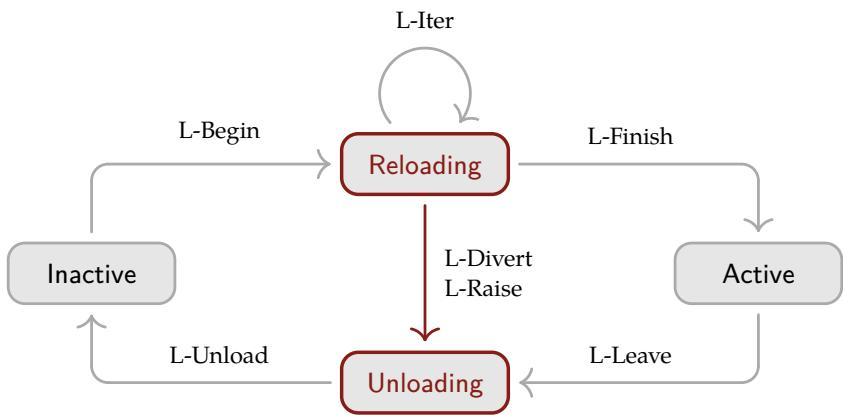
\includegraphics[keepaspectratio,alt={image}]{images/292085ac3f4ef886f94c611c14a57c3de3fd5a92462c7a5892130e190975f400.jpg}}

图 2 \textbar{} 进行中的转移生命周期；两个转移状态以轮廓框出

\subsubsection{撤回} \label{withdrawal}

第~3.2 节要求依赖者在它们的依赖之后激活，也要求依赖只在它们的依赖者停用之后撤回其供给。前半句在基础演算中已经成立：激活要求 \(\gamma \models d _ { n }\)，所以声明键 \(k\) 的纤维，在任何纤维活跃地提供 \(k\) 之前都不能激活。后半句才是实质性的，它必须交付的比状态变化的排序更多。一个因其提供者即将离开而被拆除的组件，正在运行它自己的拆除（teardown）代码，而这段代码可能需要正是被撤回的那个余效应；关闭连接池通常意味着把连接交还给提供它们的东西。后半句必须交付的是：消费者在整个停用期间仍能读取 \(k\)，且提供者对 \(k\) 的撤回只有在之后才生效。基础演算根本做不到这一点：其 L-Unload 把撤销供给与运行逆操作放在同一步中执行，在两者之间没有留下可供消费者拆除代码占据的区间。

这一层把这个步骤拆成两步，并用如下条件守卫后半句。

\textbf{定义 50.} 当某个其他已安装纤维把某个键解析到它时，纤维 \(n\) 在 \(\gamma\) 处被依赖（relied upon）：

\[
\begin{array} { r l } & { \mathrm { r e l i e d } _ { n } ( \gamma ) : = \exists m \in \mathrm { d o m } \bigl ( F _ { \gamma } \bigr ) , k \in d _ { m } . m \neq n \land \mathrm { i n s t a l l e d } _ { m } ( \gamma ) \land \omega _ { m } ( k ) = n } \\ & { \qquad \quad \frac { \theta _ { n } = \mathsf { A c t i v e } ( g , \omega ) \quad \mathrm { t a r g e t } _ { n } ( \gamma ) \neq \omega } { \gamma \longrightarrow \gamma [ \theta _ { n } \mapsto \mathsf { U n l o a d i n g } ( g , \omega , \perp ) ] } \quad \mathrm { L \cdot L e a v e } } \\ & { \qquad \quad \frac { \theta _ { n } = \mathsf { U n l o a d i n g } ( g , \omega , \zeta ) \quad \neg \mathrm { r e l i e d } _ { n } ( \gamma ) \quad g ( \gamma ) = \delta } { \gamma \longrightarrow \delta [ \theta _ { n } \mapsto \mathsf { I n a c t i v e } ( \zeta ) ] } \quad \mathrm { L \cdot U n l o a d } } \end{array}\tag{46}
\]

L-Leave 记录停用的决定而不付诸行动，这使纤维停止提供其余效应，同时保持它自己的已提交视图以及其他所有纤维的视图完好。L-Unload 应用累加器、丢弃已提交视图，并让纤维以其携带的结果处于 \(\mathsf { I n a c t i v e }\)；该结果是 \(\bot\)，直到第~4.3.4 节提供另一种情形。它是整个演算中唯一应用累加器的规则。

排序的两个半部随后由该形式的不同部分承担：可见性半部由已提交视图承担，L-Unload 将其丢弃作为最后一个动作；排序半部由前提 \(\neg \mathrm { r e l i e d } _ { n } ( \gamma )\) 承担，我们称之为守卫，它把对 \(k\) 的撤回按捺住，直到每个把 \(k\) 解析到 \(n\) 的消费者都已离开。定理~63 证明了两者。

守卫按绑定而非按纤维施加：\(\mathrm { r e l i e d } _ { n } ( \gamma )\) 检验是否有某个已提交视图点名 \(n\)，因此一个不声明 \(n\) 的任何键的纤维不构成障碍，在另一个域（第~3.2.3 节）中解析过 \(n\) 的某个键的纤维同样不构成障碍。在第~4.2 节的单一来源规约下，按绑定的读法与更粗略的检验 \(\exists m \neq n ,\ k \in d _ { m } .\ \mathrm { i n s t a l l e d } _ { m } ( \gamma ) \wedge k \in p _ { n }\) 一致——在那里，一个键只有一个可能的提供者。

这类守卫通常会死锁。使其免于死锁的是 \(\mathsf { U n l o a d i n g }\) 以及 \(\sigma _ { \gamma }\) 只取 \(\mathsf { A c t i v e }\) 纤维之表的并集：一旦 L-Leave 已标记 \(n\)，其表就离开 \(\sigma _ { \gamma }\)，于是任何目标视图都不能再点名 \(n\)，且每个已向 \(n\) 作出承诺的消费者自己也正在离开。定理~66 把它转化为"守卫总能解除"这一论断。

守卫沿余效应而非沿纤维树为停用排序：父亲可以在它的一个孩子仍处于 \(\mathsf { U n l o a d i n g }\) 时运行其逆操作，因为 relied 只涉及已提交视图。相应地，父亲与孩子之间的排序比定理~63 对提供者与其消费者的排序更弱；而那些效应在环境状态中相遇的父亲与孩子，则由定义~60 的独立性假设支配。

\subsubsection{迭代} \label{iteration}

一次激活可以依次执行多个效应，而停用必须把它们全部恢复。我们用效应迭代器（effect iterator）来建模这样的激活：其每一次迭代都产出修改后的上下文、一个逆操作和一个续体（continuation）：

\textbf{定义 51.} 把效应迭代器 \(\mathfrak { E } _ { \Gamma } ^ { \mathrm { i t e r } }\) 和带见证的效应迭代器 \(\mathfrak { E } _ { \Gamma } ^ { \mathrm { i t e r * } }\) 定义为如下递归类型：

\[
\begin{array} { r l } & { \mathfrak { E } _ { \Gamma } ^ { \mathrm { i t e r } } : = \mu \mathfrak { I } . \Gamma \to \Gamma \times ( \Gamma \to \Gamma ) \times \mathsf { M a y b e } ( \mathfrak { I } ) } \\ & { \mathfrak { E } _ { \Gamma } ^ { \mathrm { i t e r * } } : = \mu \mathfrak { I } . \left( e : \Gamma \to \Gamma \times ( \Gamma \to \Gamma ) \times \mathsf { M a y b e } ( \mathfrak { I } ) \right) } \\ & { \qquad \times \left( ( \gamma : \Gamma ) \to ( \mathbf { l e t } \ ( \delta , g , o ) = e ( \gamma ) \ \mathbf { i n } \ g ( \delta ) \simeq \gamma ) \right) } \end{array}\tag{47}
\]

其中 \(e ( \gamma )\) 产出三元组 \(( \delta , g , o )\)，分别表示：

• \(\delta\) 是新上下文；

• \(g\) 是当前效应的逆函数；

• \(o\) 指示续体：

– \(\mathsf { N o t h i n g }\) 表示迭代终止；

– \(\mathsf { J u s t } ( i )\) 提供下一次迭代。

见证按定义~33 的 $\simeq$ 来读，正如定义~37 读 \(\mathfrak { E } _ { \Gamma } ^ { * }\) 的见证那样：当 \(i\) 尊重 $\simeq$ 且其产出的每个 \(g\) 都尊重 $\simeq$ 并满足上面那条子句时，\(i \in \mathfrak { E } _ { \Gamma } ^ { \mathrm { i t e r } }\) 属于 \(\mathfrak { E } _ { \Gamma } ^ { \mathrm { i t e r * } }\)。三元组按分量比较：\(\mathsf { N o t h i n g }\) 只与 \(\mathsf { N o t h i n g }\) 比较，\(\mathsf { J u s t } ( i )\) 与 \(\mathsf { J u s t } ( i ^ { \prime } )\) 比较需当 \(i \simeq i ^ { \prime }\)；迭代器上的 $\simeq$ 是满足这些子句的最大关系。把 $\simeq$ 取为 \(\Gamma\) 上的相等，即恰好恢复该读法。

效应迭代器变换 \(\mathrm { e f f e c t } _ { \Gamma } ^ { \mathrm { i t e r } }\) 通过递归调用把 \(\mathrm { e f f e c t } _ { \Gamma }\) 扩展到迭代器结构上：

\textbf{定义 52.} 把效应迭代器变换 \(\mathrm { e f f e c t } _ { \Gamma } ^ { \mathrm { i t e r } }\) 定义为：

\[
\begin{array} { r l } & { \mathrm { e f f e c t } _ { \Gamma } ^ { \mathrm { i t e r } } : \mathfrak { E } _ { \Gamma } ^ { \mathrm { i t e r } } \to \partial \Gamma \to \partial ^ { 2 } \Gamma } \\ & { \mathrm { e f f e c t } _ { \Gamma } ^ { \mathrm { i t e r } } = i \mapsto ( \gamma , \varphi ) \mapsto \mathbf { l e t } \ ( \delta , g , o ) = i ( \gamma ) \ \mathbf { i n } \ \mathbf { l e t } \ t = \mathrm { t r a c k } _ { \Gamma } ( g , \mathrm { p r } _ { 1 } \circ i ) \ \mathbf { i n } \ \mathbf { m a t c h } \ o } \\ & { \qquad \quad | \ \mathsf { N o t h i n g } \Rightarrow ( ( \delta , \varphi \circ g ) , t ) } \\ & { \qquad \quad | \ \mathsf { J u s t } ( i ^ { \prime } ) \Rightarrow \mathbf { l e t } \ ( s , r ) = \mathrm { e f f e c t } _ { \Gamma } ^ { \mathrm { i t e r } } ( i ^ { \prime } ) ( \delta , \varphi \circ g ) \ \mathbf { i n } \ ( s , t \circ r ) } \end{array}\tag{48}
\]

在每一次迭代中，逆操作 \(g\) 按应用顺序复合到 \(\varphi\) 上，因此累加器 \(\varphi \circ g _ { 1 } \circ \cdots \circ g _ { k }\) 在应用时自然地按后进先出（LIFO）顺序恢复效应。因为 \(\mathrm { e f f e c t } _ { \Gamma } ^ { \mathrm { i t e r } }\) 落在与 \(\mathrm { e f f e c t } _ { \Gamma }\) 相同的 \(\partial \Gamma \to \partial ^ { 2 } \Gamma\) 中，迭代器本身就是一种效应，可以在任何效应可用的地方使用。组件的整个激活就是这样一个用途——这正是本节其余部分要形式化的内容——并且实现允许在每个变更点（mutation site）接受迭代器（第~5.1.1 节）。\(\mathsf { M a y b e } ( \mathfrak { E } ^ { \mathrm { i t e r } } )\) 续体在任何两次相邻迭代之间提供了边界：在该边界处，上下文就是迄今各次迭代所形成的上下文，而累加器恢复的也正是这些迭代所产生的东西，不多不少。在这个意义上，效应迭代器是一种具象化的定界续体（delimited continuation）——主流语言通过 yield 运算符暴露的那种结构 {[}43{]}——因此该模型直接对接到它们已经提供的生成器（generator）上。

在演算中，从此刻起，定义~44 的 \(e _ { n }\) 按 \(\mathfrak { E } _ { \Gamma } ^ { \mathrm { i t e r * } }\) 来读；把原子效应函数替换为迭代器，把基础 L-Reload 拆成一个迹线（trace）所经过的"已开始"状态，并给纤维一个离开该状态的第二条出路。

\[
\begin{array} { r l } & { \frac { \theta _ { n } = \mathsf { I n a c t i v e } ( \perp ) \quad \omega = \mathrm { t a r g e t } _ { n } ( \gamma ) \neq \perp } { \gamma \longrightarrow \gamma [ \theta _ { n } \mapsto \mathsf { R e l o a d i n g } ( e _ { n } , \mathrm { i d } _ { \Gamma } , \omega ) ] } \quad \mathrm { L \cdot B e g i n } } \\ & { \frac { \theta _ { n } = \mathsf { R e l o a d i n g } ( i , g , \omega ) \quad \mathrm { t a r g e t } _ { n } ( \gamma ) \neq \omega \quad ( \delta , h ) = ( \gamma , \mathrm { i d } _ { \Gamma } ) \vee i ( \gamma ) = ( \delta , h , - ) } { \gamma \longrightarrow \delta [ \theta _ { n } \mapsto \mathsf { U n l o a d i n g } ( g \circ h , \omega , \perp ) ] } \quad \mathrm { L \cdot D i v e r t } } \\ & { \frac { \theta _ { n } = \mathsf { R e l o a d i n g } ( i , g , \omega ) \quad \mathrm { t a r g e t } _ { n } ( \gamma ) = \omega \quad i ( \gamma ) = ( \delta , h , \mathsf { J u s t } ( i ^ { \prime } ) ) } { \gamma \longrightarrow \delta [ \theta _ { n } \mapsto \mathsf { R e l o a d i n g } ( i ^ { \prime } , g \circ h , \omega ) ] } \quad \mathrm { L \cdot I t e r } } \\ & { \frac { \theta _ { n } = \mathsf { R e l o a d i n g } ( i , g , \omega ) \quad \mathrm { t a r g e t } _ { n } ( \gamma ) = \omega \quad i ( \gamma ) = ( \delta , h , \mathsf { N o t h i n g } ) } { \gamma \longrightarrow \delta [ \theta _ { n } \mapsto \mathsf { A c t i v e } ( g \circ h , \omega ) ] } \quad \mathrm { L \cdot F i n i s h } } \end{array}
\]

每次迭代都按定义~52 把新产出的逆操作以 \({ \boldsymbol { g } } \circ { \boldsymbol { h } } ,\) 复合到累加器上，因此累加器按后进先出顺序应用这些逆操作。在任意两次相邻迭代之间，如果目标视图已变化，系统可以转移（divert）该转移，并应用迄今累积的逆操作来恢复上下文。与所有其他停用一样，L-Divert 经由 \(\mathsf { U n l o a d i n g }\) 走，而不是就地应用累加器；它在那里遇到的守卫是空的——一个从未处于 \(\mathsf { A c t i v e }\) 的纤维不提供任何东西，也不出现在任何已提交视图中。它的两个分支中的第一个中止纤维所持有的迭代——只有迭代边界才能使这成为可能，因此转移可以落下的粒度就是迭代器的粒度；第二个分支让该迭代落地，而第~4.3.3 节正是需要它的地方。

普通的效应函数 \(( \mathfrak { E } _ { \Gamma } )\) 是退化情形，其中第一次迭代就已产出 \(\mathsf { N o t h i n g }\)。这样的转移仍经过 \(\mathsf { R e l o a d i n g }\)，L-Divert 在那里仍然适用，但累加器是 \(\mathrm { i d } _ { \Gamma }\)，且没有任何迭代运行过，因此什么都不会被恢复，转移要么安装其全部效应，要么一个都不安装。

\subsubsection{异步} \label{asynchrony}

迄今为止的各层允许环境在两次相邻迭代之间移动，并假定每次迭代本身瞬时完成，其发起与落地是一步。我们抽象地建模这种非即时性：一次迭代产出一个类型为 \(\mathsf { F u t u r e } ( A )\) 的值，其中 \(\mathsf { F u t u r e }\) 是一个不透明的类型构造子，其定义性性质是：在提交（submission）与完成（resolution）之间，外部状态可能改变。

在这个模型下，一次迭代在一个状态发起、在另一个状态落地，纤维在飞行期间处于 \(\mathsf { R e l o a d i n g }\)。这一层添加的是惯性：一旦发起，迭代就会落地，且其落地不能被拒绝。因此，在飞行期间转向的目标视图不能通过中止迭代来回应，只剩下 L-Divert 中让迭代落地的那一分支可用：迭代落地，随后纤维停用。所以这一层不添加任何规则，也不添加任何规则所匹配的类型；在 \(\Gamma\) 的粒度上，惯性就是它的全部内容，其形式是对宿主可以采取 L-Divert 的哪个分支的限制。

那个分支正是基础演算无法表达的东西。在那里，目标视图已转向的转移在发现它的同一步中被撤销；在这里，飞行中的迭代必须先落地，所以纤维在逆操作运行期间需要一个去处，唯一可靠的地方是持有该迭代所产出逆操作的 \(\mathsf { U n l o a d i n g }\)。改走 \(\mathsf { A c t i v e }\) 会让纤维在一步的长度内提供其余效应，并迫使它的依赖者去针对一个已经离开的组件激活。这就是实现中 reload 与 unload 的相互链接。

停用也可以直接链接回激活——通过复合（composite）而非规则。L-Unload 对目标视图不携带任何前提，因此无论纤维停用期间目标视图变成了什么，累加器都会运行，纤维变为 \(\mathsf { I n a c t i v e }\)，而 L-Begin 可以从该状态立即开始一次新的转移。

\subsubsection{失败} \label{failure}

迄今的每条规则都假定它所运行的效应成功，而运行时做不到。组件安装的效应延伸到了跟踪它们的上下文之外，它们触及的东西可能拒绝：一个已绑定的端口、一个不存在的文件、一个不应答的对端。失败的转移仍必须让纤维的效应得到恢复，而不是搁浅。

令 \(\Xi\) 是一个错误集合，并精化定义~51 的效应迭代器，使迭代可以抛错（raise）而不产出三元组：

\[
\begin{array} { r l } & { \mathfrak { E } _ { \Gamma } ^ { \mathrm { f a i l } } : = \mu \mathfrak { I } . \Gamma \to \mathsf { E i t h e r } ( \Xi , \Gamma \times ( \Gamma \to \Gamma ) \times \mathsf { M a y b e } ( \mathfrak { I } ) ) } \\ & { \mathfrak { E } _ { \Gamma } ^ { \mathrm { f a i l } * } : = \mu \mathfrak { I } . \left( e : \Gamma \to \mathsf { E i t h e r } ( \Xi , \Gamma \times ( \Gamma \to \Gamma ) \times \mathsf { M a y b e } ( \mathfrak { I } ) ) \right) } \\ & { \qquad \times \left( ( \gamma : \Gamma ) \to ( \mathbf { l e t } \ \mathsf { R i g h t } ( \delta , g , o ) = e ( \gamma ) \ \mathbf { i n } \ g ( \delta ) \simeq \gamma ) \right) } \end{array}\tag{49}
\]

见证只约束 \(\mathsf { R i g h t }\) 这一情形，在模式不匹配处是空条件——一次抛错没有可撤销的东西；从此刻起，\(\mathsf { R e l o a d i n g }\) 携带的 \(i\) 按 \(\mathfrak { E } _ { \Gamma } ^ { \mathrm { f a i l } * }\) 来读。定义~52 的提升（lift）也照搬过来，只是把抛错替代三元组进行传播，因此正如普通迭代器一样，会抛错的迭代器可以在任何效应可用的地方使用。这一层添加一条规则，并把定义~49 的第二种结果投入使用，O-Remove 无需加宽即可接纳它。L-Iter、L-Finish 和 L-Divert 的前提中，它们所匹配的三元组外层都读作 \(\mathsf { R i g h t }\)。抛错是迭代所做的事情，因此这条规则是从 \(\mathsf { R e l o a d i n g }\) 退出。

\[
\frac { \theta _ { n } = \mathsf { R e l o a d i n g } ( i , g , \omega ) \quad i ( \gamma ) = \mathsf { L e f t } ( \xi ) } { \gamma \longrightarrow \gamma [ \theta _ { n } \mapsto \mathsf { U n l o a d i n g } ( g , \omega , \xi ) ] } \quad \mathrm { L \cdot R a i s e }
\]

L-Raise 先恢复后记录。纤维带着作为其结果的错误进入 \(\mathsf { U n l o a d i n g }\)，在那里应用累积到失败迭代为止的累加器，随后纤维到达 \(\mathsf { I n a c t i v e } ( \xi )\)，什么也没有安装；这个状态与中止式 L-Divert 本会产生的状态相比，只在纤维所携带的结果上不同。像所有其他停用一样处理失败，正是使每个结果只能通过 L-Unload 到达的原因，这也是定理~59 所依据的单一事实。L-Begin 以 \(\mathsf { I n a c t i v e } ( \perp )\) 为前提，因此生命周期不会从错误结果重新进入；这就是结果的实质——它扣住一个其效应函数在其运行所针对的状态中已被证明不可靠的纤维，而不是在不变的环境中对它重试。失败的纤维也不阻碍任何东西：它是 \(\mathsf { I n a c t i v e }\)，因此不携带已提交视图，也无法使 relied 成立。

失败记录在纤维上，而不是传播给其父亲，因此转移失败的组件会留下其兄弟继续运行——这正是插件宿主想要的行为，也是结果按纤维记录、而非作为整个状态属性的原因。
\subsection{元理论} \label{metatheory}

第 4.3 节提供了十条规则：第 4.2 节的三条编排规则；针对一次激活的 L-Begin、L-Iter 与 L-Finish；针对激活可能提前结束的两种方式的 L-Divert 与 L-Raise；以及针对一次去激活的 L-Leave 与 L-Unload。本节以这些规则的全局形式读出可组合性的两个维度——一个纤维的保证无论其余纤维在中间做什么都成立——并加上只有整个系统才有资格被要求的东西：系统总能到达其目标所要求的配置，而且该配置正是静态装配本会产生的那个配置。下面每一条性质都是关于一串步骤的性质，因此我们为步骤编号，并按该编号读取状态的各个字段。

本节沿用第 3.3.2 节的两项约定。下面状态之间的每一处相等都按定义 33 的观测等价 $\simeq$ 来读，正如引理 38 对第 3.1 节的那些相等性所做的那样；一个效应函数所要满足的见证条件正是定义 37 给出的那个，对迭代器按定义 51 给出的方式读，对注册迭代则在下面的 $\approx$ 下读。

定义 53. 以 $t$ 为步骤编号，使 $\gamma ^ { t }$ 是前 $t$ 步所到达的状态，并记

\[
\operatorname { s t e p } ^ { t } : = r ( n )\tag{50}
\]

表示在 $\gamma ^ { t }$ 处所采取的一步：它应用的规则 $r$（十条之一），以及它应用该规则时所处的名字 $n \in \mathfrak { N }$。序列从 $\gamma ^ { 0 }$ 开始，其中 dom $\left( F ^ { 0 } \right) = \varnothing ,$ 因此每个纤维都经由一次 O-Insert 进入存在，无论是编排者发起的还是某次迭代采取的（定义 47）。$\gamma ^ { t }$ 的每个字段把编号作为上标携带，因此 $\theta _ { n } ^ { t } , \omega _ { n } ^ { t } , \sigma _ { n } ^ { t } , g _ { n } ^ { t }$ 与 $i _ { n } ^ { t }$ 分别是 $n$ 在 $\gamma ^ { t }$ 处的生命周期状态、已提交视图、表、累加器与剩余迭代器；而 $F ^ { t }$ 与 $\sigma ^ { t }$ 则是 $\gamma ^ { t }$ 自身的注册表与余效应上下文，即在该状态下读到的定义 45 的 $F _ { \gamma }$ 与 $\sigma _ { \gamma }$。谓词把状态作为其参数、其余一切作为下标，因此 $\mathsf{installed}_{n}^{t}$、$\mathsf{target}_{n}^{t}$、$\mathsf{relied}_{n}^{t}$ 与 $\mathsf{quiet}_{n}^{t}$ 就是定义 46、定义 49 与定义 50 的谓词在 $\gamma ^ { t }$ 处的实例。$n$ 的一段活跃期（episode）是一个极大索引区间 $[ b , u ]$，在整个区间上 $\mathsf{installed}_{n}^{t}$ 成立。它在 $b$ 处开启，其中 $b > 0$ 且 $\neg \mathsf{installed}_{n}^{b - 1}$，空注册表 $F ^ { 0 }$ 使初始时没有任何纤维处于已安装状态；它在 $u$ 处关闭，此时 $\mathsf{installed}_{n}^{u}$ 而 $\neg \mathsf{installed}_{n}^{u + 1}$，最后一段活跃期不必如此。

第 4.3 节的每条规则都以 $\gamma \longrightarrow \delta [ \cdots ]$ 的形式作结：前提从 $\gamma$ 计算出 $\delta$，在没有计算任何东西的地方则把结果保留为 $\gamma$；方括号对注册表中被点名的字段进行编辑。这两半分别命名，而且两者都是定义在整个 $\Gamma$ 上的映射。在 $\gamma ^ { t }$ 处由作用于 $n$ 的规则所采取的一步，其状态映射为

\[
\Psi ^ { t } : = \left\{ \begin{array} { l l } { \mathrm { p r } _ { 1 } \circ i } & { \mathrm { a t ~ L \mathrm { - } I t e r , ~ L \mathrm { - } F i n i s h , ~ a n d ~ a ~ l a n d i n g ~ L \mathrm { - } D i v e r t } } \\ { g } & { \mathrm { a t ~ L \mathrm { - } U n l o a d } } \\ { \mathrm { i d } _ { \Gamma } } & { \mathrm { a t ~ e v e r y ~ o t h e r ~ r u l e } } \end{array} \right.\tag{51}
\]

其中 $i$ 与 $g$ 是 $\theta _ { n } ^ { t }$ 所携带的迭代器与累加器；编辑 $\mathrm{edit}^{t} : \Gamma \to \Gamma$ 则是把方括号读作一个函数，把前提在 $\gamma ^ { t }$ 处计算出的值赋给它所点名的字段。因此二者都由 $\mathrm{step}^{t}$ 连同 $\gamma ^ { t }$ 完全确定，并在每个状态上都有定义——这正是定理 61 与引理 71 得以在远离 $\gamma ^ { t }$ 处对它们求值的原因。每一步都可分解为

\[
\gamma ^ { t + 1 } = \mathrm { e d i t } ^ { t } \big ( \Psi ^ { t } \big ( \gamma ^ { t } \big ) \big )\tag{52}
\]

例如在 L-Unload 处，$\mathrm{edit}^{t}$ 就是 $[ \theta _ { n } \mapsto \mathsf{Inactive}(\zeta) ]$；在 O-Remove 处它则是移除 $\setminus n$。正因如此，后一半是一种编辑而非一次赋值。字段沿同一条接缝划分：一方面是表 $\sigma _ { m }$——一旦创建 $m$ 的 O-Insert 把它置空，任何 $\mathrm{edit}^{t}$ 都不再写它；另一方面是控制字段 $\theta _ { m } , \tau _ { m } , \pi _ { m } , d _ { m } , p _ { m } , e _ { m }$ 连同 dom $\left( F _ { \gamma } \right)$——除非经由定义 47 的原语，任何 $\Psi ^ { t }$ 都不写它们。当两个状态除控制字段外处处一致时，记 $\gamma \approx \delta$。

关系 $\approx$ 并不是定义 33 的 $\simeq$，二者谁也不细化谁，因为每一个都忘掉了另一个必须保留的东西。恢复精确性是关于效应的一种论断，因此 $\approx$ 精确地比较表与周围状态，只忘掉注册表里"哪个纤维安装了它们"的记录。规则读取控制字段以决定自己是否适用，因此 $\simeq$ 必须保留它们；本节把它读作定义 33 与以下各项一致的合取：注册表的定义域一致，且每个纤维的每个控制字段都一致：

\[
\begin{array} { r l r } { \gamma \simeq \delta } & { : = } & { \sigma _ { \gamma } \simeq \sigma _ { \delta } \wedge \mathrm { d o m } \big ( F _ { \gamma } \big ) = \mathrm { d o m } ( F _ { \delta } ) \wedge \forall n , c \in \{ \theta , \tau , \pi , d , p , e \} . c ( \gamma ( n ) ) \simeq c ( \delta ( n ) ) (53) } \end{array}
\]

函数类型的字段——如 $e _ { n }$ 与 $\theta _ { n }$ 内部的 $g$——按定义 36 比较映射的方式比较；迭代器按定义 51 比较两个迭代器的方式比较；任何其他类型的字段按相等性比较。下面的结论对这两种关系都成立，各对应状态的一半；引理 55 一劳永逸地为全部十条规则建立了 $\simeq$ 这一半。

表 1 把第 4.3 节的十条规则读作此类写入。累加器、已提交视图与剩余迭代器都是 $\theta _ { n }$ 的组成成分，因此第三列也记录对它们的写入；表中的 $h$ 指第四列的那次迭代所产生的逆，当 L-Divert 中止该迭代时则为 $\mathrm { i d } _ { \Gamma }$。当由迭代器构造的 $\Psi ^ { t }$ 注册一个纤维（定义 47）时，该注册在它抽取的名字处携带 O-Insert 行的写入；累加器使某个纤维退役的 L-Unload 则携带 O-Retire 行的写入。下面每一处情形分析都是对这张表的一次查表，其中五种查表重复出现的频率足够高，值得命名。

{\def\LTcaptype{none} % do not increment counter
\begin{longtable}[]{@{}|l|l|l|l|l|@{}}
\toprule\noalign{}
\endhead
\bottomrule\noalign{}
\endlastfoot
\hline
规则 & $\theta _ { n } ^ { t }$ & $\theta _ { n } ^ { t + 1 }$ & $\Psi ^ { t }$ & 被编辑的控制字段 \\
\hline
O-Insert & 未定义 & $\mathsf{Inactive}(\bot)$ & $\mathrm { i d } _ { \Gamma }$ & $\mathrm { d o m } \big ( F _ { \gamma } \big )$ \\
\hline
O-Retire & 无约束 & 不变 & $\mathrm { i d } _ { \Gamma }$ & $\tau _ { n }$ \\
\hline
O-Remove & $\mathsf{Inactive}(-)$ & 未定义 & $\mathrm { i d } _ { \Gamma }$ & $\mathrm { d o m } \big ( F _ { \gamma } \big )$ \\
\hline
L-Begin & $\mathsf{Inactive}(\bot)$ & $\mathsf{Reloading}(e _ { n } , \mathrm { i d } _ { \Gamma } , \omega)$ & $\mathrm { i d } _ { \Gamma }$ & $\theta _ { n }$ \\
\hline
L-Iter & $\mathsf{Reloading}(i , g , \omega)$ & $\mathsf{Reloading}(i ^ { \prime } , g \circ h , \omega)$ & $\operatorname { p r } _ { 1 } \circ i$ & $\theta _ { n }$ \\
\hline
L-Finish & $\mathsf{Reloading}(i , g , \omega)$ & $\mathsf{Active}(g \circ h , \omega)$ & $\operatorname { p r } _ { 1 } \circ i$ & $\theta _ { n }$ \\
\hline
L-Divert & $\mathsf{Reloading}(i , g , \omega)$ & $\mathsf{Unloading}(g \circ h , \omega , \bot)$ & $\mathrm { i d } _ { \Gamma }$ 或 $\operatorname { p r } _ { 1 } \circ i$ & $\theta _ { n }$ \\
\hline
L-Raise & $\mathsf{Reloading}(i , g , \omega)$ & $\mathsf{Unloading}(g , \omega , \xi)$ & $\mathrm { i d } _ { \Gamma }$ & $\theta _ { n }$ \\
\hline
L-Leave & $\mathsf{Active}(g , \omega)$ & $\mathsf{Unloading}(g , \omega , \bot)$ & $\mathrm { i d } _ { \Gamma }$ & $\theta _ { n }$ \\
\hline
L-Unload & $\mathsf{Unloading}(g , \omega , \zeta)$ & $\mathsf{Inactive}(\zeta)$ & $g$ & $\theta _ { n }$ \\
\hline
\end{longtable}
}

表 1 | 把各规则读作对它们所作用的纤维 $n$ 的写入，其中 $\mathrm{step}^{t}$ 就是把该规则应用于 $n$ 的那一步。

引理 54. 将表 1 与定义 48 一起读，则对每一步 $t$ 以及 $\gamma ^ { t }$ 中出现的所有纤维 $m$、$n$：

\begin{enumerate}
\def\labelenumi{\arabic{enumi}.}
\tightlist
\item
  仅当 step $t$ 作用于 $m$ 时才有 $\sigma _ { m } ^ { t + 1 } \neq \sigma _ { m } ^ { t }$，且该写入位于 $\Psi ^ { t }$ 内部；
\end{enumerate}

$\omega _ { n }$ 仅在 $\mathrm { s t e p } ^ { t } = \mathrm { L } \mathrm { - B e g i n } ( n )$ 处进入存在，仅当 $\mathrm { s t e p } ^ { t } = \mathrm { L } \mathrm { - U n l o a d } ( n )$ 时停止存在，因此 $\omega _ { n } ^ { t }$ 在 $n$ 的一段活跃期内保持恒定；

\begin{enumerate}
\def\labelenumi{\arabic{enumi}.}
\setcounter{enumi}{2}
\item
  仅当 step$^t$ = L-Unload($n$) 时才有 $\Psi ^ { t } = g _ { n } ^ { t }$，且没有其他步骤把 $g _ { n }$ 作用到状态上；
\item
  $\neg \mathsf{installed}_{n}^{t} \wedge \mathsf{installed}_{n}^{t + 1} \Rightarrow \mathrm { s t e p } ^ { t } = \mathrm { L } \mathrm { - B e g i n } ( n )$，且 $\mathsf{installed}_{n}^{t} \wedge \neg \mathsf{installed}_{n}^{t + 1} \Rightarrow \mathrm { s t e p } ^ { t } = \mathrm { L } \mathrm { - U n l o a d } ( n )$；
\item
  $\pi _ { n } , d _ { n } , p _ { n }$ 与 $e _ { n }$ 随 $n$ 的条目一起进入存在，此后永不再被写入；$\tau _ { n }$ 是单调的，只在 $\top$ 处、且只由 O-Retire 写入。
\end{enumerate}

证明. 设 step $t$ 在 $n$ 处应用规则 $r$。由定义 53，它可分解为 $\mathrm{edit}^{t} \circ \Psi ^ { t }$，其中 $\mathrm{edit}^{t}$ 写入表 1 第五列所点名的那些字段、此外不写别的；$\Psi ^ { t }$ 或是 $\mathrm { i d } _ { \Gamma }$，或是 $n$ 的某个迭代的一次应用，或是累加器 $g _ { n } ^ { t }$——它是那些迭代所产生的各个逆的复合。由定义 48，三者中的每一个都局限于 $n$，因此 $\Psi ^ { t }$ 除 $\sigma _ { n }$ 外不写 $\gamma ^ { t }$ 中任何纤维的字段，连同注册所添加的条目与其逆所写的 $\tau$。因此这两半把写入分割开来，而每一条款就是把这一分割读到某一个字段上。对第二列与第三列的一种读法被用到了两次：$\mathsf{Inactive}$ 是唯一不携带已提交视图的生命周期状态，L-Begin 是唯一离开它的规则，L-Unload 是唯一进入它的规则，而其余每一行都把自己前提的 $\omega$ 原封不动地带进结论。

\begin{enumerate}
\def\labelenumi{(\arabic{enumi})}
\item
  $\mathrm{edit}^{t}$ 不写任何表（第五列没有点名任何表），而 $\Psi ^ { t }$ 对出现的 $m \neq n$ 不写任何 $\sigma _ { m }$。因此 $\sigma _ { m }$ 只可能在 $m = n$ 处、且只在 $\Psi ^ { t }$ 内部发生变化。
\item
  $\omega _ { n }$ 是 $\theta _ { n }$ 的组成成分，而 $\theta _ { n }$ 只有 $\mathrm{edit}^{t}$ 才写、且只在步骤所作用的那个纤维处写，因此由上面的读法，$\omega _ { n }$ 在 $n$ 的一次 L-Begin 处进入存在，在 $n$ 的一次 L-Unload 处停止存在。$n$ 的一段活跃期是 $\mathsf{installed}_{n}$ 成立的区间，因而也是 $\omega _ { n }$ 全程有定义的区间，所以这两条规则都不会落在其内部。
\item
  看第四列：累加器只在 L-Unload 一处出现。其余规则取正向映射 $\operatorname { p r } _ { 1 } \circ i$ 或 $\mathrm { i d } _ { \Gamma }$，而任何 $\mathrm{edit}^{t}$ 根本不会把映射作用到状态上。
\item
  installed 即 $\theta _ { n } \neq \mathsf { I n a c t i v e } ( - )$；由上面的读法，L-Begin 与 L-Unload 是仅有的两条前提与结论中 $\theta _ { n }$ 是否 $\mathsf{Inactive}$ 不同的规则。作用于某个 $m \neq n$ 的步骤不写 $\theta _ { n }$，而注册所添加的条目位于 $\gamma ^ { t }$ 中不存在的名字处。
\end{enumerate}

\begin{enumerate}
\def\labelenumi{(\arabic{enumi})}
\setcounter{enumi}{4}
\tightlist
\item
  第五列没有任何一行点名 $\pi , d , p$ 或 $e$；这些字段随 O-Insert 添加的条目一起进入存在，其结论会写它们，注册采取的 O-Insert 同样如此。只有 O-Retire 写 $\tau$，且写在 $\top$ 处，无论它由编排者采取还是作为注册的逆（定义 47）；O-Insert 在尚不存在的名字处把 $\tau$ 置为 $\bot$，因此没有哪一步会把 $\tau$ 送回 $\bot$。$\blacksquare$
\end{enumerate}

还有三种进一步的查表说明规则无法看到什么。第一种是，规则只通过上面的那些观测来读取状态，因此整个演算可以下降到 $\Gamma / \simeq$。

引理 55（$\simeq$-不变性）. 设 $\gamma \simeq \gamma ^ { \prime }$ 按上面的读法成立。则第 4.3 节的一条规则在 $\gamma$ 处作用于 $n$ 适用，当且仅当它在 $\gamma ^ { \prime }$ 处作用于 $n$ 适用，且两次应用所到达的状态仍由 $\simeq$ 关联。

证明. 第 4.3 节的每条前提都属于四种之一，每一种都读取关系所保留的某个成分。把 $\theta _ { n }$ 或 $\tau _ { n }$ 与一个模式匹配的前提，以及 O-Remove 的前提 $\forall m. \pi _ { m } \neq n$，读取的是控制字段。O-Insert 的前提 $( d , p , e ) \in \mathfrak { C } _ { \Gamma }$ 与 $\forall m. p \cap p _ { m } = \emptyset$ 读取的是 $d , p$ 与 $e$。提及 $\mathsf{target}_{n}$ 或 $\mathsf{relied}_{n}$ 的前提读取的是 $\tau _ { n }$、$\theta _ { m }$ 内部的已提交视图以及 dom $\left( \sigma _ { \gamma } \right)$——后者由定义 45 从 $\theta _ { m }$ 与 dom $( \sigma _ { m } )$ 计算而来——而定义 33 只在两个余效应上下文定义域一致时才把它们关联起来。其余前提读取的是 dom $\left( F _ { \gamma } \right)$。没有任何前提以超出 $\simeq_{k}$ 的方式读取一个值 $\sigma _ { \gamma } ( k )$，因此没有任何前提能把两个 $\simeq$-相关状态区分开。

对结论而言，由定义 53 有 $\gamma ^ { t + 1 } = \mathrm { e d i t } ^ { t } \big ( \Psi ^ { t } \big ( \gamma ^ { t } \big ) \big )$。$\mathrm{edit}^{t}$ 所赋的值是它所匹配的那些前提的成分，由上面的段落与定义 51 在两个状态之间关联起来；定义 51 把迭代器在 $\simeq$-相关状态下产生的三元组关联起来。而 $\Psi ^ { t }$ 尊重 $\simeq$：它或是 $\mathrm { i d } _ { \Gamma }$，或是 $e _ { n }$ 的一次迭代（定义 51 要求迭代尊重 $\simeq$），或是 $\theta _ { n }$ 内部的累加器——由同一定义，它是若干各自尊重 $\simeq$ 的逆的复合。$\blacksquare$

一个状态携带的名字被上述观测中的两种读到：dom $\left( F _ { \gamma } \right)$ 与控制字段的索引；抽取名字的规则会抽取任何一个尚未使用的名字（定义 47）。因此在 $\simeq$ 的意义下读取下面的结论，也就要求把它们读到一重命名之下——这正是第 4.1 节的纪律的具体兑现。

引理 56（等变性）. 设 $\chi : \mathfrak { N } \to \mathfrak { N }$ 是一个双射，并设 $\chi \cdot \gamma$ 是携带注册表 $F _ { \gamma } \circ \chi ^ { - 1 }$ 的状态，其中出现在某个 $\pi _ { m }$ 或 $\omega _ { m }$ 中的每个名字都被替换为它的像。则 $\chi \cdot \gamma$ 是一个状态，且在 $\gamma$ 良构处良构；并且 $\mathrm { s t e p } ^ { t } = r ( n )$ 把 $\gamma ^ { t }$ 带到 $\gamma ^ { t + 1 }$，当且仅当 $r ( \chi ( n ) )$ 把 $\chi \cdot \gamma ^ { t }$ 带到 $\chi \cdot \gamma ^ { t + 1 }$。

证明. 前提只在把某个名字与另一个名字作比较时才读它，无论是直接比较——如 O-Insert 的新鲜性 $n \not \in$ dom $\left( F _ { \gamma } \right)$ 与 O-Remove 的 $\forall m. \pi _ { m } \neq n$——还是经由一张名字表，如 $\mathsf{target}_{n}$ 与 $\mathsf{relied}_{n}$ 读取 $\pi _ { m }$ 与 $\omega _ { m }$。双射保留每一处这样的比较。规则写入的唯一名字是 O-Insert 设置的 $\pi$ 与 L-Begin 设置的 $\omega$，二者都取自其前提所读的内容，因此这些写入与 $\chi$ 可交换；效应函数根本不写任何名字，只通过定义 47 的原语抽取一个名字，而定义 48 把该名字局限于该原语所添加的条目。良构性（定义 58）是四条把名字与名字进行比较的条件。$\blacksquare$

因此一个序列与其重命名以同样的顺序采取同样的规则，所到达的状态只相差一个 $\chi$。两个除了各自注册所抽取的名字之外一致的序列由此被等同起来，下面的结论即在识别它们的那一重命名意义下读取。

第二种查表是，一个被剥去一切、只剩名字的条目对规则不可见；正是这一点使定义 47 能在其恢复的状态中没有该纤维时让它退役，也使引理 72 得以移除一段被删除的活跃期所留下的注册。

引理 57（残留条目）. 当 $\tau _ { n } = \top$、$\theta _ { n } = \mathsf { I n a c t i v e } ( \bot )$、$\sigma _ { n } = \emptyset$，且没有任何 $m$ 使 $\pi _ { m } = n$ 时，称 $n$ 在 $\gamma$ 处为残留的；残留条目满足 $\gamma \approx \gamma \setminus n$。若 $n$ 在 $\gamma$ 处残留，则对每条规则和每个 $m \neq n$：

\begin{enumerate}
\def\labelenumi{\arabic{enumi}.}
\tightlist
\item
  在 $\gamma$ 处作用于 $m$ 的规则也在 $\gamma \setminus n$ 处作用于 $m$ 适用，且两次应用所到达的状态只在 $n$ 处的条目上不同，而该条目仍保持残留；
\item
  反之，在 $\gamma \setminus n$ 处作用于 $m$ 的规则也在 $\gamma$ 处适用，除非它是一次抽取名字 $n$ 或索取 $p _ { n }$ 的某个键的 O-Insert。
\end{enumerate}

证明. 作用于 $m \neq n$ 的规则的前提所读的任何观测中，残留的 $n$ 都不作出贡献。它不是 $\mathsf{Active}$，因此 $\sigma _ { n }$ 不进任何 $\sigma _ { \gamma }$，$n$ 也不是任何键的提供者，从而 $\gamma \models d _ { m }$ 与 $\mathsf{target}_{m}$ 都不受影响；$\mathsf{installed}_{n}$ 不成立，因此 $n$ 不向 $\mathsf{relied}_{m}$ 提供任何析取项；没有任何 $\pi _ { m ^ { \prime } }$ 点名 $n$，因此对 $m$ 的 O-Remove 的前提 $\forall m ^ { \prime } . \pi _ { m ^ { \prime } } \neq m$ 不受影响；而 $\theta _ { n } , \tau _ { n } , \pi _ { n }$ 只有作用于 $n$ 的规则才会读。条款 (2) 所排除的两个前提，正是移除所放宽的两个：不存在的名字是新鲜的，不存在的供给满足所有其余要求。由引理 54，作用于 $m \neq n$ 的规则不写 $n$ 的任何字段，因此该条目得以存活；又由定义 48，该步的状态映射局限于 $m$，因此它使 $\sigma _ { n }$ 保持为空。$\blacksquare$

简化生命周期状态、连同对它们进行匹配的规则，会得到一个子演算，而并非每条结论都能在简化后存活。去掉第 4.3.1 节正是关键情形——这是第 4.3 节开篇就做出的划分，现在从元理论一侧来看：它的护栏正是建立定义 58 的条款 (3) 与 (4) 的东西，定理 63 则依赖于该护栏所创造的区间，因此没有它这三条都会失效。其余三个小节所增加的内容可以简化掉而不影响下面的结论，它们各自只是向定义 49 所确定的同一个状态空间添加规则。

\subsubsection{保持性} \label{preservation}

定义 45 确定了注册表的形状；在下面的结论可以向其添加内容之前，必须先按它检查规则。本小节确定规则所保持的不变式，其中第一条条款就是那种形状，其余各条则是那些结论所假定的东西。

定义 58. 当对一切 $m , n \in \mathop { \mathrm { d o m } } \bigl ( F _ { \gamma } \bigr )$ 与一切 $k \in K$ 都有：

\begin{enumerate}
\def\labelenumi{\arabic{enumi}.}
\tightlist
\item
  $\pi _ { n } \in \mathrm { d o m } \bigl ( F _ { \gamma } \bigr ) \cup \{ \mathsf{root} \}$；
\item
  $m \neq n \Rightarrow p _ { m } \cap p _ { n } = \emptyset$；
\item
  $\mathsf{installed}_{n}(\gamma) \Rightarrow \omega _ { n }$ 在 $d _ { n }$ 上全定义，且取值于 dom $\left( F _ { \gamma } \right)$；
\item
  $\mathsf{installed}_{n}(\gamma) \wedge k \in d _ { n } \wedge \omega _ { n } ( k ) = m \Rightarrow \mathsf{installed}_{m}(\gamma)$。
\end{enumerate}

时，注册表 $F _ { \gamma }$ 是良构的。

条款 (1) 是把定义 45 的树逐条边读出，保证父指针落在注册表之内。该定义还要求的无环性无需单独条款，因为指针所指名的纤维总是在指名的纤维之前被注册。

定理 59（保持性）. 若 $F ^ { t }$ 良构，则无论 step $t$ 应用哪条规则，$F ^ { t + 1 }$ 都良构。每一条条款都从 $\gamma ^ { t }$ 处的全部四条在 $\gamma ^ { t + 1 }$ 处被建立。

证明. 设 step $t$ 作用于 $n$。

\begin{enumerate}
\def\labelenumi{(\arabic{enumi})}
\tightlist
\item
  由表 1，只有 O-Insert 与 O-Remove 写 $\pi$ 或 dom $\left( F _ { \gamma } \right)$。O-Insert 以 $\pi _ { n } \in \mathrm { d o m } ( F ^ { t } ) \cup \{ \mathsf{root} \}$ 为前提，这正是为它添加的纤维而设的条款；它在扩大 dom $\left( F _ { \gamma } \right)$ 的同时让其他每个 $\pi$ 保持不变。O-Remove 有前提 $\forall m. \pi _ { m } \neq n$，因此任何幸存的 $\pi _ { m }$ 都不点名它移除的那个纤维。
\end{enumerate}

\begin{enumerate}
\def\labelenumi{(\arabic{enumi})}
\setcounter{enumi}{1}
\item
  O-Insert 的最后一条前提是 $\forall m. p _ { n } \cap p _ { m } = \emptyset$，这正是为它添加的纤维而设的条款；且由表 1，没有其他规则写 $p$ 或扩大 dom $\left( F _ { \gamma } \right)$。下面用到两个推论：由定义 43 有 dom $( \sigma _ { m } ) \subseteq p _ { m }$，因此不同的表互不相交，$\sigma _ { \gamma }$ 是一个函数；且 $k \in p _ { m } \cap p _ { m ^ { \prime } }$ 迫使 $m = m ^ { \prime }$，因此 $k$ 至多有一个可能的提供者。
\item
  由引理 54(2)，写 $\omega _ { n }$ 的唯一规则是 L-Begin，其前提 $\omega = \mathsf { t a r g e t } _ { n } ^ { t } \neq \bot$ 使它在 $d _ { n }$ 上全定义且取值于 dom $\left( F ^ { t } \right)$（target 所点名的正是提供者）。由表 1，缩小 dom $\left( F _ { \gamma } \right)$ 的唯一规则是 O-Remove，其前提 $\theta _ { n } ^ { t } = \mathsf { I n a c t i v e } ( - )$ 给出 $\neg \mathsf { i n s t a l l e d } _ { n } ^ { t }$，从而由 $\gamma ^ { t }$ 处的条款 (4)，在 $\mathsf { i n s t a l l e d } _ { m } ^ { t }$ 成立时，没有任何 $m$ 对某个 $k \in d _ { m }$ 有 $\omega _ { m } ^ { t } ( k ) = n$；而 $n$ 自身不携带任何 $\omega$。
\item
  由引理 54(2) 与 (4)，该条款在 $\gamma ^ { t + 1 }$ 处只可能在以下情形失效：某个已安装者失陷、某个 $\omega$ 被写入、或者某个 $\omega$ 所指名的纤维离开了 dom $\left( F _ { \gamma } \right)$。
\end{enumerate}

最后一种情形是一次 O-Remove，其被移除的纤维未处于已安装状态，从而由 $\gamma ^ { t }$ 处的条款 (4)，它不被任何已安装的 $m$ 的 $\omega _ { m } ^ { t }$ 所点名。第一种情形是一次对 $n$ 的 L-Unload，其前提 $\neg \mathsf { r e l i e d } _ { n } ^ { t }$ 读作

\[
\forall m \neq n , k \in d _ { m } . \mathsf { i n s t a l l e d } _ { m } ^ { t } \Rightarrow \omega _ { m } ^ { t } ( k ) \neq n
\]

并且它不写任何 $m \neq n$ 的 $\omega _ { m }$，留下 $\neg \mathsf { i n s t a l l e d } _ { n } ^ { t + 1 }$，因此该条款对 $n$ 同样成立。第二种情形是一次对 $n$ 的 L-Begin，写入 $\mathsf { t a r g e t } _ { n } ^ { t }$，其值正是 $d _ { n }$ 各键的提供者，因而在 $\gamma ^ { t }$ 处处于 $\mathsf{Active}$；该步骤不改变任何其他纤维的 $\theta$，因此它们在 $\gamma ^ { t + 1 }$ 处仍处于已安装状态。$\blacksquare$

L-Unload 上的护栏正是承载条款 (3) 与 (4) 的东西。O-Remove 的前提 $\forall m. \pi _ { m } \neq n$ 只涉及父指针；使已提交视图不能点名一个被移除纤维的，是那个护栏——它在若干步之前、出于另一个原因就被施加。由于失败同样经由 $\mathsf{Unloading}$ 路由，这一论证无需针对错误结局再重复一遍。由此得出两条基础演算并不具备的结论。O-Remove 释放的名字可以被 O-Insert 重新签发，因为没有过期的已提交视图会点名它；而且一个纤维一旦处于 $\mathsf{Inactive}$ 就可以被移除，无需另加一项"没有谁依赖它"的单独检查。
\subsubsection{时间维组合性} \label{temporal-composability}

局部时间维组合性用一个累加器恢复一串效应（第~3.1.3 节）。注册表为每根纤维持有一个累加器，各纤维相互交错：在 \(n\) 将逆元合成到 \(g _ { n }\) 之上到 \(g _ { n }\) 实际运行之间，其它纤维已经移动了状态。\(g _ { n }\) 是否仍然撤销它当初被构造来撤销的东西，正是该保证的全局形式所断言的；而它所依赖的条件是：中间的那些步骤与 \(g _ { n }\) 可交换。

定义 60. 对 \(i \in { \mathfrak { E } } _ { \Gamma } ^ { \mathrm { i t e r * } }\)，令 \(\mathrm { r e a c h } ( i )\) 为包含 \(i\) 且在续延下封闭的最小迭代器集合；在某迭代器处解读定义~17 的变换幺半群 \(\mathfrak { M }\)，即取其生成元为 \(\mathrm { r e a c h } ( i )\) 中每个迭代器的前向映射与其所产出的逆元：

\[
\begin{array} { r l } & { \mathrm { r e a c h } ( i ) : = \bigcap \{ S \mid i \in S \land \forall i ^ { \prime } \in S , \gamma \in \Gamma . i ^ { \prime } ( \gamma ) = ( - , - , \mathsf { J u s t } ( i ^ { \prime \prime } ) ) \Rightarrow i ^ { \prime \prime } \in S \} } \\ & { \quad \mathfrak { M } ( i ) : = \langle \{ \mathrm { p r } _ { 1 } \circ i ^ { \prime } \mid i ^ { \prime } \in \mathrm { r e a c h } ( i ) \} \cup \{ \mathrm { p r } _ { 2 } ( i ^ { \prime } ( \gamma ) ) \mid i ^ { \prime } \in \mathrm { r e a c h } ( i ) , \gamma \in \Gamma \} \rangle } \end{array}\tag{54}
\]

在适用第~4.3.4 节之处，围绕该三元组将其读作 \(\mathsf { R i g h t }\)；并用 \(\mathrm { l e n } ( i )\) 表示 \(\mathrm { r e a c h } ( i )\) 中被续延排序的链 \(C \subseteq \mathrm { r e a c h } ( i )\) 上 \(| C |\) 的上确界。两个迭代器 \(i , j\) 独立，当且仅当它们在定义~19 的意义下独立，其中解读使用这些变换幺半群，并把一次迭代的产出理解为它的逆元连同其续延：

\[
\begin{array} { r } { \forall f \in \mathfrak { M } ( i ) , g \in \mathfrak { M } ( j ) . \quad f \circ g \simeq g \circ f \qquad } \\ { \forall i ^ { \prime } \in \mathrm { r e a c h } ( i ) , g \in \mathfrak { M } ( j ) , \gamma \in \Gamma . \quad \mathrm { p r } _ { 2 , 3 } ( i ^ { \prime } ( g ( \gamma ) ) ) \simeq \mathrm { p r } _ { 2 , 3 } ( i ^ { \prime } ( \gamma ) ) } \end{array}\tag{55}
\]

对 \(j\) 对称地成立；\(\simeq\) 在映射上的解读同定义~36，在续延上的解读同定义~51，在登记迭代（定义~47）上的解读为所指名组件的同一性。一族迭代器 \(( i _ { l } ) _ { l \in L }\) 是两两独立的，当且仅当对每个 \({ \mathit { l } } \neq { \mathit { l } } ^ { \prime }\)，\(i _ { l }\) 与 \(i _ { l ^ { \prime } }\) 独立；一个步骤序列是两两独立的，当且仅当 \(( e _ { n } ) _ { n \in N }\) 是两两独立的，其中 \(N\) 是序列曾持有的名字集合，编排器插入的每根纤维与某次迭代登记的每根纤维各对应一个名字。

这种意义下的独立正是迹理论所取为原初的概念：可交换的作用在序列上生成一个等价关系，在该关系下重排两个相邻独立作用的顺序保持端点不变 {[}44{]}，而引理~71 正是针对这些规则的重排结果。用族而非集合来使同一组件的两个名字保持在作用域内：此时条件要求该组件的效应函数与自身独立，即要求 \(\mathfrak { M } ( i )\) 可交换。第一个条件是定理~61 所用到的，第二个则是定理~73 额外需要的：重排两根纤维的步骤，等于在另一根纤维移动过的状态处对迭代器求值；而映射可交换本身并不能说明迭代器在那里产出相同的逆元与相同的续延。检验第一个条件只需迭代器本身即可，因为引理~18(1) 把可交换性从生成元传递到它们所生成的幺半群。

在这些条件下，定理~7 的单累加器不变量在交错之下依然成立，其形式正是时间维组合性的内容所在：运行一个逆元会撤回该纤维的贡献，且仅此而已。

定理 61.（恢复精确性）设步骤序列两两独立，设 \(n\) 的一段进程在 \(b\) 处开启，设 \(u \geq b\) 位于其中，并设 \(t _ { 1 } < \dots < t _ { l }\) 是 \([ b , u )\) 中作用纤维不是 \(n\) 的那些下标。则

\[
g _ { n } ^ { u } ( \gamma ^ { u } ) \approx \big ( \Psi ^ { t _ { l } } \circ \dotsb \circ \Psi ^ { t _ { 1 } } \big ) \big ( \gamma ^ { b } \big )\tag{56}
\]

也就是说，在 \(\gamma ^ { u }\) 处应用 \(n\) 的累加器，所得的（在控制字段的意义下）正是同样的那些步骤从 \(\gamma ^ { b }\) 出发本来会产生的状态。若把右端解读为「\(n\) 从未开始」时所达到的状态，则还需额外假设：没有 \(n\) 所登记的纤维在 \([ b , u )\) 内走一步，因为 \(n\) 登记出的纤维是不会在场去走那一步的。

证明。对 \(u\) 归纳，遍及那些满足 \(u+1\) 在进程中的下标 \(u\)。当 \(u = b\) 时，\(b - 1\) 处的步骤是一个 L-Begin（进程由定义~53 开启），于是按表~1 有 \(g _ { n } ^ { b } = \mathrm { i d } _ { \Gamma }\)，下标集为空，断言即为 \(\gamma ^ { b } \approx \gamma ^ { b }\)。每一步使用两个事实。由于 \(\mathrm { e d i t } ^ { t }\) 只写控制字段，\(\gamma ^ { t + 1 } \approx \Psi ^ { t } ( \gamma ^ { t })\)；又由于 \(\mathfrak { M } ( e _ { n } )\) 中除登记所添加者外，每个映射都不写控制字段，由定义~48 连同定义~47，这样的每个映射都把 $\approx$-相等的状态映到 $\approx$-相等的状态。

设步骤 \(u\) 作用于 \(n\)。由于进程在 \(u\) 与 \(u+1\) 处均开启，引理~54(4) 排除了作用于 \(n\) 的 L-Begin 与 L-Unload；而 O-Insert 与 O-Remove 读取一个被 \(\mathrm { i n s t a l l e d } _ { n } ^ { u }\) 否定的 \(\theta _ { n }\)，于是剩下两种情况。当规则为 L-Iter、L-Finish 或落地型 L-Divert 时，表~1 给出 \(\Psi ^ { u } = \mathrm { p r } _ { 1 } \circ i _ { n } ^ { u }\)，以及 \(g _ { n } ^ { u + 1 } = g _ { n } ^ { u } \circ h\)，其中 \(h\) 是该迭代产出的逆元。定义~51 的见证条件给出 \(h ( \Psi ^ { u } ( \gamma ^ { u } ) ) = \gamma ^ { u }\)，在迭代登记纤维之处（引理~57）则精确到 $\approx$；而 \(g _ { n } ^ { u }\) 按上面的等式保持 $\approx$，因此

\[
g _ { n } ^ { u + 1 } \big ( \gamma ^ { u + 1 } \big ) \approx \big ( g _ { n } ^ { u } \circ h \big ) \big ( \Psi ^ { u } \big ( \gamma ^ { u } \big ) \big ) = g _ { n } ^ { u } \big ( \gamma ^ { u } \big )
\]

当规则为 L-Leave、L-Raise、中止型 L-Divert 或作用于 \(n\) 的 O-Retire 时，表~1 给出 \(\Psi ^ { u } = \mathrm { i d } _ { \Gamma }\) 与 \(g _ { n } ^ { u + 1 } = g _ { n } ^ { u }\)，于是同一等式在 \(h = \mathrm { i d } _ { \Gamma }\) 时成立。无论哪种情形，归纳假设都在下标集不变的情况下传递下去，这正是定理~7 的运算逐步进行的过程。

设步骤 \(u\) 作用于 \(m \neq n\)。则按表~1 有 \(g _ { n } ^ { u + 1 } = g _ { n } ^ { u }\)；且 \(\Psi ^ { u } \in \mathfrak { M } ( e _ { m } )\)，或当规则为编排规则时 \(\Psi ^ { u } = \mathrm { i d } _ { \Gamma }\)，于是独立性给出

\[
g _ { n } ^ { u } \bigl ( \gamma ^ { u + 1 } \bigr ) \approx g _ { n } ^ { u } \bigl ( \Psi ^ { u } ( \gamma ^ { u } ) \bigr ) = \Psi ^ { u } \bigl ( g _ { n } ^ { u } \bigl ( \gamma ^ { u } \bigr ) \bigr )
\]

这就是附加上 \(\Psi ^ { u }\) 之后的归纳假设。□

推论 62.（终端恢复）设步骤序列两两独立，设 \(n\) 的一段进程在 \(b\) 处开启并在 \(u\) 处关闭，无论 \(n\) 到达何种结局。则，取 \(t _ { 1 } < \cdots < t _ { l }\) 如定理~61，

\[
\gamma ^ { u + 1 } \approx \bigl ( \Psi ^ { t _ { l } } \circ \cdots \circ \Psi ^ { t _ { 1 } } \bigr ) \bigl ( \gamma ^ { b } \bigr )\tag{57}
\]

由 O-Remove 移除的纤维同样不留任何痕迹，因为其前提只允许 \(\theta _ { n } = \mathsf { I n a c t i v e } ( - )\)。

证明。由引理~54(4)，步骤 \(u\) 是作用于 \(n\) 的 L-Unload，其 \(\Psi ^ { u }\) 按引理~54(3) 为 \(g _ { n } ^ { u }\)，于是 \(\gamma ^ { u + 1 }\) $\approx$ \(g _ { n } ^ { u } ( \gamma ^ { u } )\)，定理~61 适用。陈述与 $\approx$ 都不涉及 \(\zeta\)，而按表~1，\(\zeta\) 正是 L-Divert 与 L-Raise 所导致状态相异的那个唯一字段。□

上述结果假定组件两两独立，而第~3.3.2 节正是兑现这一假定的地方：当组件执行的每个效应都是某个键上的运算、且每个键都可交换时，由这些运算构造出的任意两个效应函数都独立（定理~42）。把该结果从效应函数带到迭代器无需任何新东西：以余效应为中介的效应函数（定义~41）已经按照每一阶段所产出的结果来决定其后接续的内容，而这正是迭代器在其续延中所携带的东西。第~3.2 节的余效应运算则是完全无需任何假定的情形：组件在那里贡献的映射是集合运算与相应限制的复合，只要两个这样的映射触及不相交的键，它们就可交换；而定义~58 第 (2) 款使不同纤维的供给互不相交。

\subsubsection{空间维组合性} \label{spatial-composability}

局部空间维组合性把组件约束到它自身的规约上，只在其依赖齐备之处才激活它，并针对这些依赖对每一次上下文变化进行分类（第~3.2.2 节）。全局形式则增加了对其它纤维的量化：提供者只有在每一个解析了某绑定的依赖者都已停用之后，才会撤回该绑定；而转移据以安装其效应的解析不会在其下方漂移。余效应侧的两个性质分别交付这两条，且它们被一起证明，因为它们是同一个不变量的两半，即引理~54(2) 所确立的 \(\omega _ { n }\) 在一段进程上的固定性。排序定理是该固定性在进程的——\(n\) 处于 Active 然后处于 Unloading——那一部分上买来的结果，相干定理则是它在 \(n\) 正在安装其效应的那一部分上买来的结果。

定理 63.（排序）一根纤维只在它的依赖齐备之处才开始一次转移：

\[
{ \mathrm { s t e p } } ^ { t } = { \mathrm { L } } \mathrm { - B e g i n } ( m ) \Rightarrow \gamma ^ { t } \models d _ { m }\tag{58}
\]

再设 \([ b ^ { \prime } , u ^ { \prime } ]\) 是 \(m\) 的一段进程，满足对某个 \(m \neq n\) 和 \(k \in d _ { m }\) 有 \(\omega _ { m } ^ { b ^ { \prime } } ( k ) = n\)；设 \([ b , u ]\) 是包含 \(b ^ { \prime }\) 的 \(n\) 的进程；并设 \(t\) 遍取 \([ b ^ { \prime } , u ^ { \prime } ]\)。则

\begin{enumerate}
\def\labelenumi{\arabic{enumi}.}
\item
  \(\omega _ { m } ^ { t } ( k ) = n ;\)
\item
  \(b < b ^ { \prime }\)，且若 \([ b , u ]\) 关闭则 \(u ^ { \prime } < u\)；
\item
  \(k \in \mathrm { d o m } ( \sigma _ { n } ^ { t } )\) 且 \(\sigma _ { n } ^ { t } ( k ) = \sigma _ { n } ^ { b ^ { \prime } } ( k )\)
\end{enumerate}

证明。第一个断言正是 L-Begin 的前提 \(\mathrm { t a r g e t } _ { m } ^ { t } \neq \perp\)，由定义~46 得 \(\gamma ^ { t } \models d _ { m }\)。

(1) 即引理~54(2)。

对于 (2)，在 \(b ^ { \prime } - 1\) 处的 L-Begin 写入 \(\omega _ { m } ^ { b ^ { \prime } } = \mathrm { t a r g e t } _ { m } ^ { b ^ { \prime } - 1 }\)，其值都是提供者，所以 \(\theta _ { n } ^ { b ^ { \prime } } = \mathsf { A c t i v e } ( - , - )\)；在 \(b - 1\) 处的 L-Begin 则留下 \(\theta _ { n } ^ { b } = \mathsf { R e l o a d i n g } ( - , - , - )\)，因此 \(b \neq b ^ { \prime }\)，进而 \(b < b ^ { \prime }\)，两段进程都按定义~53 开启。设 \([ b , u ]\) 关闭，并假设 \(u \leq u ^ { \prime }\)。则 \(u \in [ b ^ { \prime } , u ^ { \prime } ]\)，于是 \(\mathrm { i n s t a l l e d } _ { m } ^ { u }\) 成立，且由 (1) 得 \(\omega _ { m } ^ { u } ( k ) = n\)；这正是 \(\mathrm { r e l i e d } _ { n } ^ { u }\)，而它在 \(u\) 处的 L-Unload 予以否定。因此 \(u ^ { \prime } < u\)。

对于 (3)，\(n\) 是在 \(\gamma ^ { b ^ { \prime } }\) 处 \(k\) 的提供者，所以 \(k \in \mathrm { d o m } \bigl ( \sigma _ { n } ^ { b ^ { \prime } } \bigr )\)。没有作用于 \(n\) 的 L-Unload 落在 \([ b ^ { \prime } , u ^ { \prime } ]\) 内：若 \([ b , u ]\) 关闭，则由 (2) 它落在 \(u > u ^ { \prime }\) 处；若 \([ b , u ]\) 不关闭，则引理~54(4) 使 \(n\) 根本没有 L-Unload。既然 \(\theta _ { n } ^ { b ^ { \prime } } = \mathsf { A c t i v e } ( - , - )\)，表~1 于是在 \([ b ^ { \prime } , u ^ { \prime } ]\) 内只留下 L-Leave 作为可以作用于 \(n\) 的唯一规则，且其 \(\Psi ^ { t }\) 为 \(\mathrm { i d } _ { \Gamma }\)；由引理~54(1)，\(\sigma _ { n }\) 在其中为常数。□

跨越多个步骤的转移，否则可能会安装针对一个在其下方已发生变化的解析所计算出的效应；两个前提防止了这一点。L-Iter 与 L-Finish 携带 \(\mathrm { t a r g e t } _ { n } ( \gamma ) = \omega\)，因此只有在已提交视图仍是其目标视图时，转移才会继续进行；L-Divert 携带其否定，因此目标视图的任何变化都会把纤维带出转移。L-Raise 则完全不依赖目标视图，因为 raise 是迭代自己做的事情，而非环境所要求的，且它在任何情况下都会退出转移。变化的两个方向并不被区分：依赖已消失的组件与依赖被替换掉的组件走同一条离开路径，因为已变成 \(\bot\) 的目标视图与已变成某个其它纤维的目标视图，同样地不等于 \(\omega\)。

惯性（inertia）正是阻止这成为关于每一步之保证的东西。当目标视图转变时已经处于飞行中的迭代无论如何都会落地，经由 L-Divert；而那一次落地会安装一个针对已不再成立的解析计算出的效应。因此规则所交付的是一个析取，而第二个分支正是使第一个分支安全的东西。

定理 64.（解析相干性）设 \(n\) 的一段进程 \([ b , u ]\) 在 \(b\) 处开启，且 \(\omega _ { n } ^ { b } = \omega\)。则 \(\theta _ { n }\) 在进程的一个初始区间 \([ b , r ]\) 上为 \(\mathsf { R e l o a d i n g } ( - , - , - )\)，且转移的每一次迭代都针对同一个解析 \(\omega\) 运行：

\[
\forall t \in [ b , r ] . \ \mathrm { s t e p } ^ { t } \in \ \{ \mathrm { L } \mathrm { - } \mathrm { I t e r } ( n ) , \mathrm { L } \mathrm { - } \mathrm { F i n i s h } ( n ) \} \Rightarrow \mathrm { t a r g e t } _ { n } ^ { t } = \omega\tag{59}
\]

当纤维离开该区间，即 \(r < u\) 时，以下二者恰有其一成立：

\begin{enumerate}
\def\labelenumi{\arabic{enumi}.}
\item
  \(\mathrm { s t e p } ^ { r } = \mathrm { L } \mathrm { - F i n i s h } ( n )\) 且 \(\theta _ { n } ^ { r + 1 } = \mathsf { A c t i v e } ( - , \omega )\)；
\item
  \(\mathrm { s t e p } ^ { r } \in \{ \mathrm { L } \mathrm { - D i v e r t } ( n ) , \mathrm { L } \mathrm { - R a i s e } ( n ) \}\)，且进程在某个 \(u > r\) 处关闭，满足 \(\gamma ^ { u + 1 }\) $\approx$ \(\left( \Psi ^ { t _ { l } } \circ \cdots \circ \Psi ^ { t _ { 1 } } \right) \left( \gamma ^ { b } \right)\)，如推论~62。
\end{enumerate}

证明。在 \(b - 1\) 处的 L-Begin 写入 \(\mathsf { R e l o a d i n g }\)，且按表~1 它是进入该生命周期状态的唯一规则；其前提 \(\theta _ { n } = \mathsf { I n a c t i v e } ( \bot )\) 与引理~54(4) 把它的任何第二次应用排除在进程之外。因此 \(\mathsf { R e l o a d i n g }\) 占据 \([ b , u ]\) 的一个初始区间 \([ b , r ]\)，并且不会被再次进入。

第一个断言因而是表~1 赋予 L-Iter 与 L-Finish 的前提 \(\mathrm { t a r g e t } _ { n } ( \gamma ) = \omega ^ { \prime }\)，再加上由引理~54(2) 得到的 \(\omega ^ { \prime } = \omega\)。

对于这个二分，\(\mathrm { s t e p } ^ { r }\) 是一个其前提具有 \(\theta _ { n } = \mathsf { R e l o a d i n g } ( - , - , - )\)、而其结论不具有该形式的规则；在表~1 中这样的规则有 L-Finish、L-Divert 与 L-Raise：第一个落入 \(\mathsf { A c t i v e } ( - , \omega )\)，另外两个落入 \(\mathsf { U n l o a d i n g } ( - , \omega , - )\)，由引理~54(4)，L-Unload 是唯一的出口，而推论~62 提供相应的等式。落地型 L-Divert 所贡献的迭代是 \(n\) 自己的迭代之一，因而在累加器所撤回的映射之列。相反，若 \(r = u\)，则序列以转移仍在飞行中而告终，此时所断言的只有第一个断言。□
\subsubsection{进展性} \label{progress}

把提供方的撤出推迟到其依赖者消失之后的守卫，只有在其最终释放时才能给出定理~63。
登记处各纤维上的一个关系承载了这一论证。

定义 65. 登记处名字上的优先关系定义为

\[
n \prec m := p_{n} \cap d_{m} \neq \emptyset \tag{60}
\]

使得 \(n\) 可以提供 \(m\) 所声明的键。它只读取 \(d\) 和 \(p\)，而由引理~54(5)，这两个字段
随纤维条目的出现而存在，之后不再被写入。

定理~66 和定理~73 都是在 \(\prec\) 无环的假设下建立的；这是假设而非定义本身给出的性
质——对于声明了自身所提供的键的组件，\(n \prec n\) 成立。\(\prec\) 所排序的是两个纤维的
激活而非它们的存续期：\(n \prec m\) 表示 \(n\) 必须首先变为 \(\mathsf{Active}\)，\(m\) 才能如
此；而提供方比其消费方存活更久则是定理~63(2)，一个关于带守卫演算的定理。

纤维的目标视图既响应创建它的纤维，也响应它的提供方。创建者通过定义~47 的原语写入的
是 \(\tau_{n}\)，而由引理~54(5)，\(\tau\) 是单调的。因此创建者在其子纤维的整个存续期内至
多能转动其子纤维的目标视图一次。

进展性断言某条规则可应用，因此它针对宿主必须提供的规则来表述：L-Begin、L-Leave、
L-Unload、着陆规则 L-Iter、L-Finish 和 L-Raise，以及 L-Divert。它从不诉诸 L-Divert 的中止
分支，因此受第 4.3.3 节惯性约束的宿主也被涵盖。

定理 66. （进展性。）假设 \(\prec\) 无环、对每个 \(n\) 有 \(\mathrm{len}(e_{n}) \leq K\)、且定
义~60 中的名字集合 \(N\) 有限；并设每一步都应用某条生命周期规则。记 \(S(n)\) 为作用在
\(n\) 上的步数，记

\[
V(n) := \left| \left\{ t : \mathrm{target}_{n}^{t} \neq \mathrm{target}_{n}^{t+1} \right\} \right| \tag{61}
\]

为其目标视图转动的次数。则

\begin{enumerate}
\def\labelenumi{\arabic{enumi}.}
\item
  （无死锁。）\(\neg \mathrm{quiet}^{t}\) 蕴含在 \(\gamma^{t}\) 处有某条生命周期规则可应用；
\item
  （终止性。）\(S(n) \leq (K+4)(V(n)+1)\)，且 \(V(n)\) 与 \(\sum_{n} S(n)\) 均为有限。
  从而每条极大生命周期步序列都结束于一个静息状态。
\end{enumerate}

证明。无死锁。设 \(\neg \mathrm{quiet}^{t}\) 成立，则某纤维 \(n\) 不满足定义~49 中静息的任一
条款。对照表~1 的四种情形，它可以是：

\begin{itemize}
\item
  \(\theta_{n}^{t} = \mathsf{Inactive}(\bot)\) 且 \(\mathrm{target}_{n}^{t} \neq \bot\)：
  L-Begin 可应用；
\item
  \(\theta_{n}^{t} = \mathsf{Reloading}(-,-,\omega_{n})\) 且 \(\mathrm{target}_{n}^{t} =
  \omega_{n}\)：L-Iter、L-Finish 和 L-Raise 中由 \(i_{n}^{t}(\gamma^{t})\) 的值所选中的那条可
  应用；
\item
  \(\theta_{n}^{t} = \mathsf{Reloading}(-,-,\omega_{n})\) 且 \(\mathrm{target}_{n}^{t} \neq
  \omega_{n}\)：若 \(i_{n}^{t}(\gamma^{t})\) 抛出，则 L-Raise 可应用；否则由 L-Divert 应用，
  令该次迭代着陆而非中止；
\item
  \(\theta_{n}^{t} = \mathsf{Active}(-,\omega_{n})\) 且 \(\mathrm{target}_{n}^{t} \neq \omega_{n}\)：
  L-Leave 可应用。
\end{itemize}

设没有任何纤维属于以上四类，于是剩下某个满足 \(\theta_{m_{0}}^{t} =
\mathsf{Unloading}(-,-,-)\) 的 \(m_{0}\)。按如下方式构造 \(m_{0}, m_{1}, \ldots\)：给定处
于 \(\mathsf{Unloading}\) 的 \(m_{j}\)，要么 \(\neg \mathrm{relied}_{m_{j}}^{t}\)，此时 L-Unload
可作用于 \(m_{j}\)，构造停止；要么存在 \(m_{j+1} \neq m_{j}\) 和 \(k_{j}\)，使得
\(\mathrm{installed}_{m_{j+1}}^{t}\) 且 \(\omega_{m_{j+1}}^{t}(k_{j}) = m_{j}\)。在后一种情形
下

\[
k_{j} \in d_{m_{j+1}} \cap \operatorname{dom}\Big(\sigma_{m_{j}}^{t}\Big) \subseteq d_{m_{j+1}} \cap p_{m_{j}}
\]

第二个成员关系是定理~63(3) 应用于 \(m_{j+1}\) 中 \(t\) 所处的那个片段，从而
\(m_{j} \prec m_{j+1}\)。此外 \(\mathrm{target}_{m_{j+1}}^{t} \neq \omega_{m_{j+1}}^{t}\)：处
于 \(\mathsf{Unloading}\) 的纤维位于定义 \(\sigma_{\gamma}\) 的并集之外，因此在 \(\gamma^{t}\)
处 \(k_{j}\) 要么未被提供，要么由 \(m_{j}\) 之外的纤维提供。若 \(m_{j+1}\) 处于
\(\mathsf{Active}\) 或 \(\mathsf{Reloading}\)，则它将属于已被排除的四类之一，所以它处于
\(\mathsf{Unloading}\)，构造继续。\(m_{j}\) 序列按 \(\prec\) 递增，从而由无环性各不相等，而
\(\operatorname{dom}(F^{t})\) 有限，所以构造停止。

终止性。两条断言界定 \(S(n)\)。

\begin{enumerate}
\def\labelenumi{(\Alph{enumi})}
\item
  在某个使 \(\mathrm{target}_{n}^{t}\) 恒等于 \(\omega^{*}\) 的极大区间上，至多有 \(K+4\) 步
  作用于 \(n\)。读取表~1 的 \(\theta_{n}\) 列：从 \(\omega \neq \omega^{*}\) 的
  \(\mathsf{Active}(-,\omega)\) 出发，纤维执行一次 L-Leave 和一次 L-Unload，然后，若
  \(\omega^{*} \neq \bot\)，执行一次 L-Begin 和至多 \(\mathrm{len}(e_{n}) \leq K\) 次着陆，
  若最后一次着陆是 L-Raise，则还有第二次 L-Unload；从针对 \(\omega \neq \omega^{*}\) 的
  \(\mathsf{Reloading}\) 出发，它用一次 L-Divert 代替 L-Leave；从任何其他状态出发，它执行
  上述序列的一个后缀。在该区间内不会再有 L-Divert 或 L-Leave，因为 L-Begin 所写入的
  \(\omega\) 正是 \(\mathrm{target}_{n}^{t} = \omega^{*}\) 本身；而在 \(\mathsf{Active}(-,\omega^{*})\)
  处、\(\omega^{*} = \bot\) 时的 \(\mathsf{Inactive}(\bot)\) 处以及 \(\mathsf{Inactive}(\xi)\) 处，
  没有任何规则可应用。
\item
  若 \(\mathrm{target}_{n}^{t} \neq \mathrm{target}_{n}^{t+1}\) 且步 \(t\) 作用于 \(m\)，则要
  么 \(m \prec n\)，要么步 \(t\) 写入 \(\tau_{n}\)。由定义~46，target 的值是 \(\tau_{n}\) 与
  \(d_{n}\) 中键的提供方的表的一个函数；提供方满足 \(k \in \operatorname{dom}(\sigma_{m})
  \cap d_{n}\)，从而 \(m \prec n\)，而由引理~54(1)，表只会在作用于其自身纤维的步上变化。
  在第一种情形中无环性给出 \(m \neq n\)，而引理~54(5) 的单调性允许第二种情形在每个纤维
  上至多发生在一个 \(t\) 处。
\end{enumerate}

由 (A)，区间计数将 \(S(n)\) 界定为 \(S(n) \leq (K+4)(V(n)+1)\)；由 (B)，target 的每一次
转动要么消耗严格位于 \(n\) 之下 \(\prec\) 序中的某个纤维的一步，要么就是 \(\tau_{n}\) 所提供
的唯一一次转动，因此 \(V(n) \leq 1 + \sum_{m \prec n} S(m)\)。由于 \(\prec\) 无环且 \(N\) 有
限，递归

\[
B(n) := (K+4)\left( 2 + \sum_{m \prec n} B(m) \right)
\]

是良基的，并定义出满足 \(S(n) \leq B(n)\) 的 \(B\)；从而 \(V(n)\) 有限，且
\(\sum_{n} S(n) \leq \sum_{n} B(n)\)。由 (1)，任何无法继续扩展的序列都是静息的。\(\square\)

\(N\) 的有限性是假设而非推导出来的，组件上的一个条件即可给出它。宿主所持有的组件是在
一切运行之前给定的有限多个程序，因此，若没有任何组件能够——哪怕是间接地——注册一个
注册了自身实例的组件的纤维，那么这些注册构成一棵有界深度的树，而
\(\mathrm{len}(e_{n}) \leq K\) 界定了它的分支。该假设排除的是无界地注册自身实例的组件。

target 记录的是提供纤维而不是一个布尔值；在第 4.2 节的单源约定下，二者驱动相同的转移，
因为那里每个键至多有一个可能的提供方。该视图买来的是上述结果的词汇：定理~63 和定
理~64 都谈到纤维激活时针对的解析，也正是这一点使这些结果在 3.2.3 节的作用域解析下仍
然成立——在那里一个键在不同领域可解析到不同提供方，供给不再强制该视图。实现承载了这
一作用域，并将视图保存在 fiber.committed 中（见 5.1.3 节）。

\subsubsection{合流性} \label{confluence}

迄今为止的结果都是关于单个纤维的。刻画系统整体性质的特性是：其动态历史不留下任何痕
迹——无论一个运行中的系统经历过怎样的激活与去激活序列，它静息时所在的状态，正是同
样的插入与退役操作在下列情形下会产生的那个状态：每个最终处于激活状态的组件都按依
赖顺序被加载一次，并且从不被卸载。生命周期关系是合流的，它所收敛到的范式正是静态组
装出来的那个。就动态组合而言，这相当于变更传播为增量计算所确立的、与从头求值相一致
的性质 {[}45{]}。

该断言只关于 \(\longrightarrow\)。编排步是输入，给定不同输入的两条序列落在不同位置并无有
趣的原因；问题在于，生命周期规则——它们在下一步作用于哪个纤维、以及处于
\(\mathsf{Reloading}\) 的纤维走哪个出口上都是非确定的——能否被弄得彼此分歧。

首先需要三条引理。第一条不参照任何步序列就确定最终处于 \(\mathsf{Active}\) 的纤维集合，
这正是使它成为输入而非调度的函数的原因。

定义 67. 当纤维在 \(\gamma\) 处未被退役、注册它的纤维受支撑、且它声明的每个键都由某个
受支撑的纤维提供时，称该纤维在 \(\gamma\) 处受支撑。\(\operatorname{dom}(F_{\gamma})\) 上的支
撑关系是上述两条款所读取的两个关系的并，

\[
m \vartriangleleft n := m \prec n \vee \pi_{n} = m \tag{62}
\]

并且在它良基之处（引理~68），我们把支撑集，即在 \(\gamma\) 处受支撑的纤维，记作 \(A\)：

\[
n \in A := \lnot \tau_{n} \land (\pi_{n} = \mathsf{root} \lor \pi_{n} \in A) \land \forall k \in d_{n}.\, \exists m \in A.\, k \in p_{m} \tag{63}
\]

其中 \(\pi_{n} = \mathsf{root}\) 标记编排器插入的纤维，而 \(\pi_{n}\) 否则指其激活注册了
\(n\) 的纤维。这些条款除 \(\tau, \pi, d, p\) 外不读取任何字段。两个半边都把纤维关联到紧
挨其下的纤维——是父级而非祖先，是直接提供方而非传递提供方，因为条款读取的正是这些；
当后续结果需要某种序时，它们取传递闭包，其极小元、极大元和线性化与
\(\vartriangleleft\) 的相同。

这些条款引用了 \(A\) 本身，因此该定义是沿 \(\vartriangleleft\) 的递归，而正是下面这条使它成
为一个有解的递归。

引理 68. （支撑是良基的。）设 \(\prec\) 无环，且 \(\gamma\) 由一条步序列到达。则
\(\vartriangleleft\) 是良基的，且 \(A\) 是定义~67 的唯一解，一个仅由 \(\tau, \pi, d, p\) 决定
的函数。

证明。按注册每个名字的步的索引来排序 \(\operatorname{dom}(F_{\gamma})\) 中的名字，定义~53
通过让序列从空登记处开始提供了这一索引。\(\vartriangleleft\) 的父级半边沿该索引下降：
O-Insert 以 \(\pi \in \operatorname{dom}\big(F_{\gamma}\big)\) 为前提，因此父指针所指向的纤维注
册得更早，迭代该指针可在有限步内到达一个名字的全部祖先。因此一个环必须使用
\(\prec\)，而由于 \(\prec\) 无环，它必须混合两者，这就需要某个 \(m\) 声明一个由 \(m\) 自身
子树中的某纤维提供的键。这样的纤维由 \(m\) 或 \(m\) 的某个后代的激活注册，因此在
\(m\) 的 L-Begin 之后的一步注册；该 L-Begin 以 \(\gamma \models d_{m}\) 为前提，所以在它之
前提供该键的纤维已是 \(\mathsf{Active}\)，而定义~58 的第 (2) 款使该键不可能有第二个提供
方。因此那个会闭合环的纤维永远不会被注册，这条边不在 \(\operatorname{dom}(F_{\gamma})\) 中。
良基递归有唯一解，且这些条款只读取四个字段。\(\square\)

最后一条读取 \(p\)，即组件可能提供的键；而 target 读取 \(\operatorname{dom}(\sigma_{\gamma})\)，
即其纤维已安装的键，定义~43 仅通过 \(\operatorname{dom}(\sigma_{n}) \subseteq p_{n}\) 将二者关
联。因此支撑集在一般情况下过度近似 \(\mathsf{Active}\) 纤维，而弥合这一差距的条件如下。

定义 69. 当组件的某个完成的激活已安装 \(p\) 中的每一个键，使得在实例化它的每个
\(\mathsf{Active}\) 纤维处 \(\operatorname{dom}(\sigma_{n}) = p_{n}\) 时，称组件 \((d, p, e)\)
在其供给上是完全的。

与独立性（定义~60）一样，这是只作用于组件的条件，不涉及任何生命周期状态或步；而独
立性已经界定了它可能失效到何种程度：如果某个组件只在另一个组件的效应所及的上下文
状态中才安装某个键，那么它的前向映射就无法与那个组件的前向映射交换，因此纤维安装
的键由它的组件而非调度决定。完全性所增加的是：这个确定的集合是全部 \(p\)，而不是它
的真子集。

引理 70. （静息时的支撑。）设 \(\prec\) 无环、\(\mathrm{quiet}(\gamma)\) 成立、\(\gamma\) 中没有
纤维失败，且 \(\gamma\) 的每个组件在其供给上完全（定义~69）。则支撑集就是
\(\mathsf{Active}\) 纤维的集合：

\[
A = \{ n : \theta_{n} = \mathsf{Active}(-,-) \} \tag{64}
\]

证明。记右端为 \(A^{\prime}\)。由于没有纤维失败，定义~49 的静息只留下
\(\mathsf{Inactive}(\bot)\) 和 \(\mathsf{Active}\) 两种状态，并给出

\[
n \in A^{\prime} \Longleftrightarrow \mathrm{target}_{n}(\gamma) \neq \bot
\]

由定义~46，右端恰在 \(\neg \tau_{n}\) 且每个 \(k \in d_{n}\) 都位于
\(\operatorname{dom}(\sigma_{\gamma})\) 中时成立，而由定义~69，
\(\operatorname{dom}(\sigma_{\gamma}) = \bigcup_{m \in A^{\prime}} p_{m}\)。中间那条正是 target
不再承载的条款，由注册来提供：\(\pi_{n} \neq \mathsf{root}\) 的纤维只由 \(\pi_{n}\) 的激活
注册，若 \(\pi_{n} \notin A^{\prime}\)，则 \(\pi_{n}\) 不是 \(\mathsf{Active}\)，于是它的累加器
已经运行，并按定义~47 使 \(n\) 退役，给出 \(\tau_{n}\)。因此 \(A^{\prime}\) 满足定义~67 的
各条款，而引理~68 给出唯一解，所以 \(A = A^{\prime}\)。\(\square\)

引理 71. （换位。）设各步两两独立且 \(F^{t}\) 良构，并设步 \(t\) 和 \(t+1\) 作用于不同纤
维 \(m\) 和 \(n\)。

\begin{enumerate}
\def\labelenumi{\arabic{enumi}.}
\tightlist
\item
  若两者都应用激活规则，即 L-Begin、L-Iter 或 L-Finish，且步 \(t+1\) 在 \(\gamma^{t}\) 处可
  应用，则步 \(t\) 在步 \(t+1\) 从 \(\gamma^{t}\) 产生的状态处可应用，且两种次序到达相同的
  \(\gamma^{t+2}\)；
\item
  若步 \(t\) 在 \(m\) 处应用激活规则、步 \(t+1\) 在 \(n\) 处应用编排规则，且步 \(t\) 不注
  册 \(n\)，则二者同样成立。
\end{enumerate}

证明。对 (1)，由表~1，\(m\) 的步写入 \(\theta_{m}\)，并在 \(\Psi^{t} \in \mathfrak{M}(e_{m})\)
之内写入表 \(\sigma_{m}\) 和效应部分。因此它不碰 \(\theta_{n}\) 和 \(i_{n}\)，且由定义~60 的
第二条条件，也不碰 \(i_{n}\) 所产出的逆与续体，所以只需检查步 \(t+1\) 中提及
\(\mathrm{target}_{n}\) 的前提。其退役半边不会失效，因为没有激活规则写入 \(\tau\)。其解析
半边也不能变动：步 \(t+1\) 在 \(\gamma^{t}\) 处可应用使每个 \(k \in d_{n}\) 都位于
\(\operatorname{dom}(\sigma^{t})\) 中，而定义~58 的第 (2) 款使提供这样的 \(k\) 的纤维成为唯
一可能的提供者，因此 \(k \notin p_{m}\)，对 \(\sigma_{m}\) 的任何写入都不会触及 \(d_{n}\) 中
的键。反向的同样论证使步 \(t\) 保持可应用。最后，由定义~60 的第一条条件，
\(\Psi^{t} \in \mathfrak{M}(e_{m})\) 与 \(\Psi^{t+1} \in \mathfrak{M}(e_{n})\) 交换，且两次编辑
写入的是不同纤维的控制字段，所以无论哪种次序，复合结果都相同。

对 (2)，由表~1，编排步有 \(\Psi^{t+1} = \mathrm{id}_{\Gamma}\)，因此两个状态映射完全交换；
它的编辑 \(\mathrm{edit}^{t+1}\) 只在 \(n\) 处写入 \(\tau_{n}\) 或
\(\operatorname{dom}(F_{\gamma})\)，激活步既不读取也不写入这些：激活步的前提读取
\(\theta_{m}, i_{m}, \tau_{m}\) 和 \(\mathrm{target}_{m}\)，而插入新 \(n\) 的 O-Insert 不移动任
何 target——新纤维不提供任何东西；而对 \(n\) 的 O-Retire 或 O-Remove 使 \(\sigma_{\gamma}\)
保持原样——在一种情形下 \(n\) 处于 \(\mathsf{Inactive}\)，在另一种情形下它的表不受影响。所
以步 \(t\) 保持可应用。反之，编排步的每个前提要么在 \(n\) 处读取（步 \(t\) 不写入那里），
要么是 O-Insert 的两个前提之一——更小的登记处只会放松这些前提——因此它在
\(\gamma^{t+1}\) 处的可应用性蕴含它在 \(\gamma^{t}\) 处的可应用性；这里正是步 \(t\) 不注册
\(n\)，才使 \(n\) 在 O-Retire 和 O-Remove 要求它出现之处仍存在于 \(\gamma^{t}\)。\(\square\)

引理 72. （删除。）设步序列两两独立、每个组件在其供给上完全（定义~69）、它到达一个
无纤维失败的静息状态 \(\gamma^{T}\)、\([b, u]\) 是 \(n\) 的一个闭合的片段、序列中没有满足
\(n \prec m\) 的 \(m\) 的片段闭合、且 \(n\) 在 \([b, u]\) 期间注册的任何纤维都没有片段。记
这些注册所抽取的名字为 \(R\)。那么，删除 \([b, u]\) 中作用于 \(n\) 的步，连同作用于 \(R\)
中某个名字的每一步，得到一条步序列，它到达的状态与 \(\gamma^{T}\) 在 \(\approx\) 意义下相等，
且在 \(R\) 之外与它 \(\simeq\) 意义下相等。

证明。被删除的步让状态保持原样。设 \(t_{1} < \cdots < t_{l}\) 是 \([b, u]\) 中作用于 \(n\) 之
外纤维的步。推论~62 给出

\[
\gamma^{u+1} \approx \bigl( \Psi^{t_{l}} \circ \cdots \circ \Psi^{t_{1}} \bigr) \bigl( \gamma^{b} \bigr)
\]

其右端正是 \([b, u]\) 中幸存的步自行产生的结果：\(\gamma^{b-1} \approx \gamma^{b}\)，且它们的
编辑写入的是删除不触及的、\(n\) 之外纤维的控制字段。由表~1，\(n\) 的被删除步不写入
\(\theta_{n}\) 之外的任何字段，而引理~54(4) 在 \(u\) 处把它恢复到 \(\mathsf{Inactive}(\bot)\)
（没有纤维失败），且它在 \(\gamma^{b-1}\) 处正是这个值。

一个不变量承载着后缀。把幸存步在对应于点 \(t\) 处到达的状态记为 \(\gamma^{\prime t}\)。我
们断言：对每个 \(t > u\)，\(\gamma^{t} \approx \gamma^{\prime t}\)；\(R\) 中的每个名字在
\(\gamma^{t}\) 处都是残留的、在 \(\gamma^{\prime t}\) 中不存在；两个状态在 \(R\) 之外的每个
名字的每个字段上都一致。在 \(t = u+1\) 处，这由上一段连同定义~47 给出：定义~47 使
\(R\) 中的每个名字被在 \(u\) 处运行的累加器退役、处于 \(\mathsf{Inactive}(\bot)\) 且持有空
表——由假设，\(R\) 的纤维没有片段。归纳步是对 \(R\) 中每个名字依次应用引理~57(1)：作
用于 \(R\) 之外的步在两个状态处有相同的前提，到达再次满足 \(\approx\) 的状态，并使 \(R\)
的条目保持残留。作用于 \(R\) 中某个名字的步属于被删除者，而引理~57(2) 说明了为什么必
须删除而非保留——对不存在名字的 O-Retire 或 O-Remove 没有纤维可作用；同样由 (1)，这
样的步不移动 \(R\) 之外的任何字段，所以丢弃它保持不变量。因此最终状态满足 \(\approx\)，
且在 \(R\) 之外相等。

没有任何幸存步失去前提。作用于 \(m \notin R \cup \{n\}\) 的步只通过
\(\mathrm{target}_{m}(\gamma)\) 或 \(\mathrm{relied}_{m}(\gamma)\) 读取 \(n\)。前者在 \(m\) 声
明 \(n\) 提供的键时依赖 \(n\)，从而 \(n \prec m\)；也在 \(n\) 注册了 \(m\) 时依赖 \(n\)，这
使 \(m \in R\)。在第一种情形下，由假设，\(m\) 的片段不闭合，所以它在 \(\gamma^{T}\) 处是打
开的；在那里静息给出 \(\omega_{m} = \mathrm{target}_{m}^{T}\)，而引理~70 把它的值归入
\(\mathsf{Active}\) 纤维——而 \(n\) 不是 \(\mathsf{Active}\)；由于一个键至多有一个可能的提供
方，\(n\) 在 \(m\) 的 L-Begin 时也没有提供 \(d_{m}\) 中的任何键。后者只通过 \(\omega_{n}\) 的
值读取 \(n\)，而删除该片段只会使 \(\mathrm{relied}\) 变为假，这放宽了 L-Unload 上的守卫而
不是阻塞它。这样的步对 \(R\) 中某个名字的读取由不变量涵盖。两两独立性是效应函数的性
质，所以删除步保持它。\(\square\)

定理 73. （合流性。）设一条步序列到达一个无纤维失败的静息状态 \(\gamma^{T}\)，各步两两独
立、每个组件在其供给上完全（定义~69），且 \(A\) 如定义~67 中那样。则

\begin{enumerate}
\def\labelenumi{\arabic{enumi}.}
\item
  （规范形。）\(\gamma^{T}\) 可以从 \(\gamma^{0}\) 出发由一条序列到达——除归约所撤回其条目的
  那些名字不计——该序列按原顺序执行相同的编排步：作用于编排器插入的纤维的编排步位
  于每个生命周期步之前，其余每个编排步位于注册其作用纤维的那一步之后；并且，对
  \(A\) 的一个使 \(\vartriangleleft\) 线性化的枚举 \(n_{1}, \ldots, n_{k}\)，按该顺序取每个
  \(n_{i}\) 的一个片段。
\item
  （合流性。）任何两条从 \(\gamma^{0}\) 出发、执行相同编排步的此类序列，经过如引理~56 那
  样的重命名后，到达由 \(\simeq\) 和 \(\approx\) 关联的状态。
\end{enumerate}

证明。对 (1)，序列的片段有两类：闭合的，以及在 \(\gamma^{T}\) 处仍打开的——后者由静息
\(\mathrm{quiet}^{T}\) 和引理~70 可知是 \(A\) 中每个纤维各一个片段。

闭合片段优先处理，对其个数做归纳。每个阶段在片段仍闭合的纤维中选取一个在
\(\vartriangleleft\) 序下极大的纤维 \(n\) 的闭合片段；由引理~68 和 \(N\) 的有限性，这样的片段
存在。于是引理~72 的三个假设都满足。由极大性，没有任何满足 \(n \prec m\) 的 \(m\) 有闭
合片段。而 \(n\) 在 \([b, u]\) 期间注册的纤维也没有片段：这样的纤维被在 \(u\) 处运行的累
加器退役（定义~47），并由引理~54(5) 保持退役，所以它的目标视图为 \(\bot\)，引理~70 把
它置于 \(A\) 之外，从而它在 \(\gamma^{T}\) 处没有打开的片段；且 \(\vartriangleleft\) 通过它的父
指针把它与 \(n\) 关联，所以由极大性它也没有闭合片段。引理移除了该片段以及它所注册名
字的各步，使 \(\gamma^{T}\) 除那些名字之外保持原样。测度减一，所以不再有闭合片段。

\(A\) 之外的纤维不取任何生命周期步。由引理~70 和静息 \(\mathrm{quiet}^{T}\)，它在
\(\gamma^{T}\) 处没有打开的片段，而现在也不再有闭合片段，所以它根本没有片段，并始终处
于 \(\mathsf{Inactive}(\bot)\)；L-Begin 是那里唯一可应用的规则，而应用它会打开一个片段。

接下来处理编排步。作用于编排器插入的纤维的编排步，由引理~71(2) 可越过另一纤维的生
命周期步向前移动一位；该引理适用是因为 \(A\) 中某纤维的步不会注册这样的名字：注册抽
取的都是新名字，而这里的名字是原始序列中某次 O-Insert 引入的。与同一纤维的生命周期
步之间则无可交换：\(n\) 的 O-Insert 已经位于 \(n\) 的每一步之前，而 \(n\) 的 O-Retire 或
O-Remove 只作用于 \(A\) 之外，后者不取生命周期步。依次把每个编排步移到最前保持它们
的相对顺序。作用于某次激活所注册的纤维的编排步不能移到最前——它的前提要求该纤维
在场——所以它停留在注册所放的位置；由上一段它作用于 \(A\) 之外，因此由引理~71 的同
一款，它与自身和注册之间的所有步都交换。

片段被排序并连续化，对 \(|A|\) 做归纳。设 \(n_{1}\) 在 \(A\) 中 \(\vartriangleleft\)-极小。则
\(d_{n_{1}} = \emptyset\) 且 \(\pi_{n_{1}} = \mathsf{root}\)，因为定义~67 把 \(d_{n_{1}}\) 中键
的一个提供方和注册 \(n_{1}\) 的纤维放入 \(A\)，而 \(\vartriangleleft\) 把二者都放在 \(n_{1}\) 之
下。所以 \(\mathrm{target}_{n_{1}}\) 不读取另一纤维的任何字段，并且——不再有编排步来写
\(\tau_{n_{1}}\)，也没有 \(n_{1}\) 之下的纤维来使它退役——它恒为常数。作用于 \(n_{1}\) 的每
一步都是激活步，没有片段闭合，且其剩余前提读取 \(\theta_{n_{1}}\) 和 \(i_{n_{1}}\)——由表~1，
只有 \(n_{1}\) 写入这些；因此每一步在每个更早的状态处都可应用，而引理~71 在不移动端点
的前提下把它向前移一位。每次应用都使 \(n_{1}\) 的一步之前的其他纤维步数减一，所以
\(n_{1}\) 的片段变成一个初始的连续块。该论证在紧随该块之后的后缀上对
\(A \setminus \{n_{1}\}\) 重复：在那里 \(n_{1}\) 全程处于 \(\mathsf{Active}\) 且不再取步，所以它
也贡献一个常数 target。这样产生的枚举按构造使 \(\vartriangleleft\) 线性化。

对 (2)，两条序列都通过 (1) 归约到某条规范序列，而两次归约在同一个（差一个重命名的）
\(A\) 上进行。定义~67 读取 \(\tau, \pi, d, p\)，其中后三个字段随纤维条目的出现而只写一次
（引理~54(5)），因此需要看清的是：相同的名字带着相同的 \(d, p, \pi\) 出现，且相同的名
字被退役。插入操作按假设为两条序列所共有。注册操作也为二者共有：\(A\) 中某纤维的一
次激活在其每次迭代中注册迭代器在那里点名的组件，而定义~60 的第二条条件使这一点在
交错中保持不变，所以 \(A\)-纤维之下的注册树是该纤维组件的函数；这些注册所抽取的名
字并不共有，正是在这里应用引理~56，用双射匹配两棵树。而一次退役要么是编排步（共
有），要么是累加器执行的 O-Retire，后者退役的恰好是同一次激活所注册的名字。使
\(\vartriangleleft\) 线性化的两个枚举只相差对不可比片段的换位，而引理~71 再次使端点保持不
变，所以两条规范序列一致。结合定理~66 的终止性，生命周期关系因此具有唯一的范式。
\(\square\)

失败被排除在陈述之外，因为它是分歧的真实来源，而且不应把这套演算解读为否认失败：
一步是否抛出取决于它运行时所处的状态，因此一个调度可能使某纤维失败，而另一个调度
完成它，两个静息状态于是会在该纤维的生命周期状态上不同。由推论~62，它们在除此之外
的任何方面都没有差异——该推论把失败纤维对状态的贡献置为无。

在第 4.2 节的基础演算中同样的定理成立，证明除了去掉一条款外无需任何替换。那里的
L-Unload 不带守卫，所以引理~72 的最后一段是空洞的；该引理的其余部分只诉诸静息
\(\mathrm{quiet}^{T}\)，基础演算原样提供之。

正是这条定理使我们可以像对待静态组装的应用那样对 Cordis 应用进行推理。一个添加组件、
移除组件、替换提供方并撤销替换的编排器，保证会到达它在一开始就把最终组合写下来所
得的状态；而组件作者在推理哪些余效应在作用域内时，可以只针对静息状态进行推理。它
也界定了这一保证的范围：它说的是状态，而不是系统沿途产生的排放，这正是第 6.1 节在
边界内部被追踪的获取与跨越边界的排放之间所作的区分。
\section{实现与案例研究} \label{implementation-and-case-study}

本节介绍 Cordis，它将第~3 节的各形式模型落实为一种实用的编程抽象。Cordis 是时空可组合性的元框架：与面向特定领域（例如 Web 路由、ORM、UI 渲染）的应用框架不同，它不规定任何具体场景；它的唯一职责是提供通用的动态组合语义。实现分为三层：(1) 核心库（第~5.1 节）直接实现效应与余效应系统；(2) 组件加载器（第~5.2 节）在核心之上扩展出配置调和与热模块替换；(3) 应用框架（例如 Koishi，第~5.3 节）在前两层之上构建领域特定功能。

\subsection{核心库} \label{core-library}

表~2 总结了理论构件与其运行时对应物之间的对应关系。特别地，本节通篇使用下文引入的运行时名称，而把理论符号保留给形式对应关系。我们还用 @@name 表示框架内部的符号键，因此 ctx{[}@@store{]} 中的方括号表示对上下文上不透明槽位的符号键访问，而不是对字符串键映射的下标访问。

Table 2 \textbar{} 理论到实现的对应关系

{\def\LTcaptype{none} % do not increment counter
\begin{longtable}[]{@{}|l|l|@{}}
\toprule\noalign{}
\endhead
\bottomrule\noalign{}
\endlastfoot
\hline
理论（第 3 节、第 4 节） & 实现 \\
\hline
\textbackslash Gamma \_ \{ \textbackslash infty \} & ctx，一等上下文 \\
\hline
\textbackslash gamma \textbackslash in \textbackslash Gamma & 上下文树以及运行系统所触及的一切 \\
\hline
\textbackslash mathfrak \{ E \} \_ \{ \textbackslash Gamma \} , \textbackslash mathfrak \{ E \} \_ \{ \textbackslash Gamma \} \^{} \{ \textbackslash mathrm \{ i t e r \} \} & 返回 / 产生逆的效应回调 \\
\hline
\textbackslash mathrm \{ e f f e c t \} \_ \{ \textbackslash Gamma \} ( e ) & ctx.effect(callback) \\
\hline
\textbackslash Sigma , \textbackslash Sigma \^{} \{ \textbackslash mathrm \{ i s o \} \} , \textbackslash Sigma \^{} \{ \textbackslash mathrm \{ i n t e r \} \} & ctx{[}@@store{]}, ctx{[}@@isolate{]}, ctx{[}@@intercept{]} \\
\hline
\textbackslash operatorname* \{ g e t \} ( k ) , \textbackslash operatorname* \{ s e t \} ( k , v ) & ctx.get(key), ctx.set(key, value) \\
\hline
\textbackslash mathrm \{ i s o l a t e \} ( k , r ) & ctx.isolate(key, realm) \\
\hline
\textbackslash operatorname \{ i n t e r c e p t \} ( k , \textbackslash nu ) & ctx.intercept(key, metadata) \\
\hline
\textbackslash langle d , p , e , \textbackslash pi , \textbackslash sigma , \textbackslash tau , \textbackslash theta \textbackslash rangle & fiber，\textbackslash mathfrak \{ C \} \_ \{ \textbackslash Gamma \} 中一个组件的实例化 \\
\hline
\textbackslash mathrm \{ d o m \} \textbackslash big ( F \_ \{ \textbackslash gamma \} \textbackslash big ) & 通过 ctx.registry 枚举 \\
\hline
n : \textbackslash mathfrak \{ N \} & fiber.uid \\
\hline
d : \textbackslash mathfrak \{ D \} \_ \{ \textbackslash Gamma \} & fiber.inject \\
\hline
p : \textbackslash mathfrak \{ P \} \_ \{ \textbackslash Gamma \} & 组件的 provide \\
\hline
e : \textbackslash mathfrak \{ E \} \_ \{ \textbackslash Gamma \} \^{} \{ * \} & fiber.apply \\
\hline
\textbackslash pi : \textbackslash mathfrak \{ N \} & fiber.parent.fiber.uid，即拥有其被实例化所在上下文的那个 fiber \\
\hline
派生实现（定义 27） & fiber.ctx，纤维运行所在的子上下文 \\
\hline
$\theta$（定义 44） & fiber.state，生命周期状态，其 LOADING 为 Reloading、FAILED 为 Inactive(ξ) \\
\hline
recover，累加器 g & fiber.dispose，累加器 \\
\hline
ω（定义 44） & fiber.committed，已提交视图 \\
\hline
provide \textbackslash mathrm \{ r \} \_ \{ k \} ( \textbackslash gamma ) & 一个 provider 纤维为 ACTIVE 的 Impl \\
\hline
target ( \textbackslash gamma , n ) & fiber.target，由 refresh 重算（算法~5），其中 $\bot$ 为 INACTIVE \\
\hline
Future、惯性（第 4.3.3 节） & fiber.inertia，进行中转移的句柄 \\
\hline
O-Insert、O-Retire（定义 47） & ctx.use 及其回调的逆（算法~4） \\
\hline
O-Remove & 从其运行时中移除、uid 被清除的纤维 \\
\hline
L-Begin、L-Iter、L-Finish & execute 的迭代循环（算法~1） \\
\hline
L-Divert & 迭代边界处守卫失败（算法~1），或 reload 链入 unload \\
\hline
L-Leave & refresh 将纤维标记为 UNLOADING（第 10 行） \\
\hline
L-Unload & unload 及其惯性链接（算法~5） \\
\hline
L-Unload 上的守卫 & unload 等待被通知的依赖者（第 25 行） \\
\hline
L-Raise & 记录在纤维上的错误，其 target 置为 $\bot$ \\
\hline
\end{longtable}
}

本节其余部分自下而上地构建核心库。第~5.1.1 节实现可逆效应，这是上下文被变更所经过的唯一原语；第~5.1.2 节在它之上实现响应式余效应；第~5.1.3 节把两者组合进组件生命周期；第~5.1.4 节则暴露基于它们构建的上下文级操作。

\subsubsection{效应追踪} \label{efect-tracking}

本节实现可逆效应（第~3.1 节）。Cordis 中每次上下文变更都流经一个单一原语 ctx.effect：余效应供给、组件实例化以及所有其他变更上下文的操作都归结为一次 ctx.effect 调用，因此任何经由上下文执行的操作都会被自动追踪，并在组件卸载时得到恢复。从操作层面看，ctx.effect 是 effectiter（定义~52）的实现：它接受一个类型为 \({ \mathfrak { E } } _ { \Gamma } ^ { \mathrm { i t e r } }\) 的回调，把它提升到 \({ \mathfrak { E } } _ { \partial \Gamma } ^ { \mathrm { i t e r } }\)，产出一个 dispose 闭包，调用该闭包即可恢复效应。Cordis 通过这一个操作同时接受 \(\mathfrak { E } _ { \Gamma }\) 与 \({ \mathfrak { E } } _ { \Gamma } ^ { \mathrm { i t e r } }\)（即席多态）；我们以迭代器形式为代表，因为普通效应函数只是产生单个逆的退化迭代器。该操作不检查的是 \({ \mathfrak { E } } _ { \Gamma } ^ { * }\) 所携带的见证：回调提供逆，而"该逆能恢复它所伴随的效应"是组件作者的责任，而非运行时验证的性质。演算在定理~61 处诉诸这一点，而第~6.1 节界定了这一责任。

算法~1 展示 ctx.effect 的构造。我们用 \(f \circ g\) 表示先运行 \(g\)、再运行 \(f\) 的处置器，用 id 表示空操作；因此每前置一个新逆便得到 LIFO 恢复。

算法~1 效应追踪
1 async function execute(callback, guard)
2 iter $\leftarrow$ callback()
3 inverse $\leftarrow$ id
4 while guard()
5 (value, done) $\leftarrow$ await iter.next()
6 if value then inverse $\leftarrow$ value $\circ$ inverse
7 if done then break
8 return inverse
9 function effect(ctx, callback)
10 armed $\leftarrow$ true
11 task $\leftarrow$ execute(callback, () $\mapsto$ armed)
12 async function dispose()
13 if not armed then return
14 armed $\leftarrow$ false
15 recover $\leftarrow$ await task
16 recover()
17 ctx.dispose $\leftarrow$ dispose $\circ$ ctx.dispose
18 return dispose

执行引擎 execute 把回调作为效应迭代器（\( \mathfrak { E } _ { \Gamma } ^ { \mathrm { i t e r } }\)，定义~51）来驱动，并把每一步产生的逆折叠成一个复合逆。在每一步之前它都咨询调用方提供的守卫；一旦守卫跳闸，迭代停止，只留下迄今已累积的逆。这正是第~4.3.2 节的步边界中断：\(\mathsf{Maybe}( \mathfrak { E } ^ { \mathrm { i t e r } } )\) 续延由迭代器的 done 标志连同守卫实现。

ctx.effect 是 execute 之上的一层薄包装，增加了两件事。其一，自处置：守卫报告 armed 标志，返回的 dispose 把 armed 翻转为 false，这同时中止任何进行中的迭代，并使恢复至多触发一次。触发两次会在某个从未施加效应的状态下应用逆，而没有任何东西约束它去撤销什么。其二，父组合：dispose 被前置到外层上下文已累积的逆 ctx.dispose 之前，因此子效应的逆本身又是父上的一个效应，这正是 \(\partial ^ { 2 } \Gamma\) 的递归结构。组件层（第~5.1.3 节）复用同一个 execute，只是守卫改为检验 fiber.target 的稳定性而非 armed。

\subsubsection{余效应操作} \label{coefect-operations}

本节实现响应式余效应（第~3.2 节）。所有余效应操作都作用于每个上下文携带的三个符号键槽位：

• @@store：值存储 \(\sigma : ( r : R ) \rightharpoonup \mathcal { V } _ { r }\)，从领域符号到类型化值的部分函数；

• @@isolate：领域表 \(\rho : \operatorname { M a p } ( K , R )\)，从余效应键到领域符号；

• @@intercept：拦截表 \(\iota : ( k : K ) \to \mathcal { M } _ { k }\)，为每个键分配它的元数据。

前两个槽位组合成两层解析 \(k \to \rho ( k ) \to \sigma ( \rho ( k ) )\)：ctx.get(key)（算法~2）先从 @@isolate 读出领域符号 \(\rho ( k )\)，再从 @@store 读出绑定值 \(\sigma ( \rho ( k ) )\)。\(\rho\) 这一间接层让隔离可以把一个键重定向到独立的绑定；而 @@intercept 只在绑定被访问时才被查阅，调整的是它的使用方式而非解析结果。我们分两部分实现这些操作：(1) 供给与通知，安装或撤回绑定并把变更传播给依赖者；(2) 隔离与拦截，重塑一个键的解析方式。

供给与通知。由于 set\(( k , v )\) 具有类型 \(\mathfrak { E } _ { \Sigma }\)（第~3.1 节），余效应供给就是一次 ctx.effect 调用，并继承其自动追踪与恢复。算法~2 实现 ctx.set(key, value)，即具体的 set\(( k , v )\)：回调在领域符号 \(\rho ( k )\) 之下把一个值绑定进存储，返回的 dispose 函数则移除它。安装与移除都会调用 notify 把变更传播给依赖组件。

算法~2 余效应操作
1 function get(ctx, key)
2 realm $\leftarrow$ ctx{[}@@isolate{]}{[}key{]} $\triangleright$ $\rho ( k )$
3 return ctx{[}@@store{]}{[}realm{]} $\triangleright$ $\sigma ( \rho ( k ) )$
4 function set(ctx, key, value)
5 function callback()
6 realm $\leftarrow$ ctx{[}@@isolate{]}{[}key{]} $\triangleright$ $\rho ( k )$
7 ctx{[}@@store{]}{[}realm{]} $\leftarrow$ value $\triangleright$ $\sigma [ \rho ( k ) \mapsto v ]$
8 notify(ctx, {[}key{]})
9 return function()
10 delete ctx{[}@@store{]}{[}realm{]} $\triangleright$ $\sigma \setminus \rho ( k )$
11 notify(ctx, {[}key{]})
12 return ctx.effect(callback)

算法~3 通过如下方式把每个绑定变更传播给依赖者：对每个存活的纤维，检验某个变更的键是否出现在它的 fiber.inject 中、并解析到同一个领域；若是，则调用 refresh（第~5.1.3 节）让该纤维针对新状态重新求值，并返回被重新求值的纤维，使调用方可以等待它们。这正是定义~26 的响应式分类：翻转满足状况的变更会激活或停用纤维，而 refresh 的幂等性使中性变更变得无害。这种重新求值与多种控制流的交互在第~5.1.3 节展开。

算法~3 响应式通知
1 function notify(ctx, keys)
2 affected $\leftarrow$ $\emptyset$
3 for fiber in all\_fibers do
4 for key in keys do
5 if key $\in$ fiber.inject and fiber.ctx{[}@@isolate{]}{[}key{]} = ctx{[}@@isolate{]}{[}key{]} then
6 refresh(fiber)
7 affected $\leftarrow$ affected $\cup$ \{fiber\}
8 break
9 return affected

一个绑定只有当安装它的纤维处于 ACTIVE 时才算对依赖者可用，因此 refresh 让每个声明键针对某个活跃提供者而非仅针对存储来解析。这正是定义~46 的 provided by 关系，也是让一次撤回在它实际发生前一步就被依赖者看到的原因：一个已进入 UNLOADING 的提供者已经停止提供，因此它的依赖者重算出一个不满足的目标视图，并在其绑定全部仍然就位时就启动自身的拆除。

隔离与拦截。这两个操作在结构上做的是同一件事：各自派生一个子上下文，针对某个键调整一张继承来的表，而让父上下文保持不变，因此恢复是隐式的：丢弃子上下文即可，无需运行任何显式逆。ctx.isolate(key, realm) 用 realm 覆盖领域映射 \(\rho\)，缺省时用一个新生成的符号（实现 isolate，定义~29），因此两个把不同符号赋给同一键的上下文会解析到独立的绑定。ctx.intercept(key, metadata) 把元数据并入拦截表 \(\iota\)（实现 intercept，定义~31）：按照该定义，新元数据与上下文已经为 key 携带的任何元数据相组合，并优先于后者。

\subsubsection{组件生命周期} \label{component-lifecycle}

组件由 ctx.use 实例化为一个纤维。本节把纤维（第~5.1 节引入）赋予第~4.3.3 节惯性状态机的操作含义。两个字段驱动下面的算法：fiber.parent，即构成组件层级（\(\Gamma _ { \infty }\) 的递归结构，第~3.3.1 节）的 fiber.ctx 的父上下文；以及 fiber.inertia，指向进行中的异步转移的句柄（空闲时为 null）。

算法~4 展示组件实例化。一个组件把余效应规格 component.inject（\(d\)）与一个效应函数 component.apply 配对；实例化把组件的 config 绑定进 fiber.apply（第 9 行），即生命周期随后运行的应用了配置的效应函数（\(e\)）。回调函数（第 2 行）是在父纤维中被追踪的效应：执行时它通过调用 refresh（算法~5）启动子生命周期；被恢复时它把子的 target 强制置为 $\bot$ 并触发 unload。这就是定义~47 的注册原语，以回调为其 O-Insert，以回调返回的闭包为其 O-Retire：实例化是父的一个普通被追踪效应，因此卸载父会级联到它的子。

算法~4 组件实例化
1 function use(ctx, component, config)
2 function callback()
3 refresh(fiber)
4 return function()
5 fiber.target $\leftarrow$ $\bot$
6 unload(fiber)
7 fiber $\leftarrow$ Fiber(parent: ctx, inject: component.inject)
8 fiber.ctx $\leftarrow$ ctx{[}fiber $\mapsto$ fiber{]}
9 fiber.apply $\leftarrow$ () $\mapsto$ component.apply(fiber.ctx, config)
10 ctx.effect(callback)
11 return fiber

算法~5 实现第~4.3.3 节的惯性状态机，其中 reload 与 unload 是惯性的：一旦进入，一次转移会运行到完成，之后系统才对目标状态的变化作出响应。它在余效应存储之上使用两个辅助查询：resolve(inject) 返回声明键当前解析到的绑定，provided(fiber) 返回该纤维所安装的绑定对应的键。refresh 函数从余效应存储重算 fiber.target，并且若纤维尚未处于转移中，则发起一次 reload 或 unload 任务\(^{2}\)。reload 函数记录当前目标并执行组件的效应函数 apply。完成后它检查目标是否仍然匹配：若是，纤维进入 ACTIVE；若否（无论新目标是 $\bot$ 还是不同的提供者集合），则链入 unload。对称地，unload 以 LIFO 顺序恢复所有被追踪的效应，然后进入 INACTIVE 或链入 reload。这一相互递归实现了惯性性质：一旦转移开始，它在任何新转移能够启动之前完成。

算法~5 组件生命周期
1 function refresh(fiber)
2 target $\leftarrow$ target($\gamma$, $n$)
3 if target = fiber.target then return
4 fiber.target $\leftarrow$ target
5 if fiber.inertia then return
6 if target ≠ $\bot$ then
7 fiber.state $\leftarrow$ LOADING
8 fiber.inertia $\leftarrow$ create\_task(reload(fiber))
9 else
10 fiber.state $\leftarrow$ UNLOADING $\triangleright$ out of service before any inverse is scheduled
11 fiber.inertia $\leftarrow$ create\_task(unload(fiber))
12 async function reload(fiber)
13 target0 $\leftarrow$ fiber.target
14 fiber.committed $\leftarrow$ resolve(fiber.inject) $\triangleright$ commit the view
15 recover $\leftarrow$ await execute(fiber.apply, () $\mapsto$ fiber.target = target0)
16 fiber.dispose $\leftarrow$ recover $\circ$ fiber.dispose
17 if fiber.target = target0 then
18 fiber.state $\leftarrow$ ACTIVE
19 notify(fiber.ctx, provided(fiber))
20 fiber.inertia $\leftarrow$ null
21 else
22 fiber.state $\leftarrow$ UNLOADING
23 fiber.inertia $\leftarrow$ create\_task(unload(fiber))
24 async function unload(fiber)
25 await all(notify(fiber.ctx, provided(fiber)).map(f $\mapsto$ f.await())) $\triangleright$ drain dependents
26 await fiber.dispose()
27 fiber.dispose $\leftarrow$ id
28 fiber.committed $\leftarrow$ $\bot$
29 if fiber.target = $\bot$ then
30 fiber.state $\leftarrow$ INACTIVE
31 fiber.inertia $\leftarrow$ null
32 else
33 fiber.state $\leftarrow$ LOADING
34 fiber.inertia $\leftarrow$ create\_task(reload(fiber))

create\_task 调度一个异步函数并发运行并返回它的句柄（存放在 fiber.inertia 中）。我们把它显式写出以保证语言无关性：在急切调度下（例如 TypeScript 的 promise），该调用是隐式的，返回的 promise 就是句柄；而在惰性调度下（例如 Python 协程、Rust future），宿主必须派生该任务它才会推进。

fiber.target 通过把每个声明键对当前余效应存储解析、并对提供它的纤维的 uid 取元组来计算，因此它是 target(\(\gamma\), \(n\))（定义~46）的一个摘要。按提供者而非按值识别绑定，正是使一次对记录目标的单一比较就足够的原因：uid 每次新取且从不复用，所以被替换的提供者不会被误认为替换它的那个，即使两者提供相等的值。由于 notify（第~5.1.2 节）在每次余效应变化时都重算目标，一个纤维恰在其某个声明键改由不同纤维提供时重新加载。原地覆盖自身绑定的提供者因此不会被观察到；想让其替换被传播的组件会撤回绑定并重新安装它。

该算法在两个互补的层面上运作。在转移层面，reload 与 unload 在完成时检查目标，从而实现跨转移的惯性链接。在每个转移内部的迭代层面，效应执行（算法~1）在每个迭代边界检查目标，从而实现在单一转移内的部分回滚。这两种机制分别对应第~4.3.3 节的转移间链接，以及定理~64 所依赖的转移内陈旧性检查。

有三行承担着定理~63 的余效应排序，而每一行所处的位置正是排序成立的原因。reload 在第 14 行提交已解析的视图，unload 则在每个逆都运行完之后才丢弃它，因此一个纤维只要处于加载状态就读到相同的绑定，它自身的拆除也不例外。refresh 在转移任务创建之前于第 10 行把纤维标记为 UNLOADING，这就是 L-Leave 步骤：纤维停止提供，依赖者在其任何逆被调度之前就据此重算。随后 unload 在第 25 行等待每个被通知的依赖者到达 INACTIVE，这就是 L-Unload 上的守卫；notify 只有在依赖者的声明键解析到与提供者相同的领域符号时才接纳它，这是守卫"依赖者必须从该纤维看到键、而不仅仅是声明它"这一要求的运行时形态。这一等待位于整个恢复之前，而非落在某个被等待的逆内部，因为 fiber.dispose 并发地发起一个纤维的各个效应，若把等待放进其中之一，其余效应就会失去次序。终止性由定理~66 保证：一个纤维只等待那些已经不再可满足的依赖者，而本身也是提供者的依赖者以同样的方式等待它自己的依赖者，因此提供者图是按需遍历的，而非预先分析。

\subsubsection{上下文访问} \label{context-access}

第~5.1.2 节的余效应操作构成一个反射式 API：余效应用 ctx.set(key, value) 写入、用 ctx.get(key) 读取，两者都以名称为键。Cordis 在这个反射式 API 之上又叠加了第二种更原生的扩展与消费上下文的方式：属性访问。组件可以把余效应作为属性 ctx{[}key{]} 来访问，仿佛它是上下文的原生结构，而非通过一次方法调用。在 TypeScript 中，Cordis 用一个 get 陷阱中介每一次属性访问的 Proxy 来实现这一点。算法~6 展示上下文如何在第~5.1.2 节原语 get 之上把这样的访问解析为一个余效应。

算法~6 代理介导的上下文访问
1 function resolve(ctx, key)
2 fiber $\leftarrow$ ctx.fiber
3 repeat
4 if key $\in$ fiber.committed then return fiber.committed{[}key{]}
5 if key $\in$ fiber.inject then throw INACTIVE\_ACCESS
6 if fiber = root then throw UNDECLARED\_ACCESS
7 fiber $\leftarrow$ fiber.parent.fiber

算法~6 从访问上下文出发向上遍历纤维链：在第一个其已提交视图绑定了 key 的纤维处，访问被授权并返回该绑定；若遍历到达一个声明了 key 却尚未提交它的纤维，则该纤维未加载，访问失败；若到达根而没有任何声明，访问作为未声明而被拒绝。这正是代理与裸 ctx.get 的差异所在：ctx.get(key) 是对存储的一次查询，返回绑定值或什么都不返回，且从不失败；而代理针对访问纤维自身的视图来解析，并在使用点强制余效应规格（\(d\)）。读取视图而非读取存储，也正是定理~63 所依赖的，因为正是这一点让某个其拆除由该依赖消失所触发的组件仍能读到该依赖。

这种拒绝是在访问点执行的运行时检查。由于组件的余效应规格（\(d\)）是静态声明的，同样的违规原则上可以在编译期检测到：在执行之前把每个 ctx{[}key{]} 对已声明的 \(d\) 解析即可。第~6.4 节讨论宿主语言的类型级依赖声明与编译期元编程如何能恰好完成这种介导。
\subsection{组件加载器} \label{component-loader}

核心库为组件开发者提供了用于动态组合的命令式原语，例如 ctx.effect、ctx.use 与 ctx.set。应用编排器则面临一个独立的问题：他们把既有组件装配成一个运行中的系统，并在其生命周期内调整组合方式。组件加载器通过引入一个声明式配置层来解决这一问题：编排器把期望的组合描述为一个持久化数据结构，而加载器把对该规范的变更转化为相应的命令式纤维操作。

61

\subsubsection{声明式配置} \label{declarative-configuration}

第~4 节把一个运行中的系统分解为若干纤维，每条纤维是某个组件的一次实例化。一次实例化所需的全部内容都可以被声明，因此编排器可以把整个系统描述为一份声明式配置：一份由加载器实现为纤维、并与之保持同步的持久化记录。

条目。一份配置由若干条目组成。每个条目指定一条纤维并管理它，绑定是双向的：加载器通过调整纤维来响应条目字段的变更；组件若修订自己的配置或停用自身，其变更会被写回它的条目。

定义~74。一个条目声明一条纤维，记录如下：

• id —— 稳定的标识符，在其所在组的子列表发生变化时用作对账键；

• url —— 要实例化的组件模块的 URL；

• isolate —— 应用到该条目上下文上的隔离注解；

• intercept —— 应用到该条目上下文上的拦截注解；

• config —— 绑定进组件、以构成其效应函数 apply 的配置；

• disabled —— 该条目是否被管理性地关闭。

一个条目之所以能充当忠实的规范，是因为支撑一条纤维的恰好就是条目所记录的内容。定义~67 的支撑集只读取 \(\tau , \pi , d ,\) 与 \(p\)，此外别无他物，而一个条目恰好给出全部四项：disabled 给出 \(\tau\)，条目在树中的父节点给出 \(\pi\)，而 url 选择声明 \(d\) 与 \(p\) 的组件。支撑集没有读取的字段是纤维的运行时状态，一次实例化同样不需要它们；引理~70 把静止状态（定义~49）的支撑集等同于 \(\mathsf{Active}\) 纤维，前提是每个组件都安装它声明的每个键（定义~69）。

这些条目构成一棵配置树，它是系统所加载内容的权威记录。一个条目可以是映射到单条纤维的叶子，其组件也可以转而加载更多组件，使该条目成为分支节点。Cordis 为这种分组与嵌套加载提供了组件：@cordisjs/group 以一组子条目作为配置，将它们作为子组加载；而 @cordisjs/include 加载一份外部配置文件（YAML 或 JSON），并把这些条目作为嵌套子树嫁接进来。两者都是建立在定义~47（算法~4）的注册原语之上的普通组件，因此嵌套树仍保持在演算之内，下文的结果对它成立。

对账。当一个条目的记录发生变更时，加载器会进行增量对账，而不是把纤维拆掉后整体重建。这种对账方式之所以可靠，其理由由元理论给出。

• 定理~73 使静止状态成为最终配置的单一函数：无论加载器在途中执行了哪些实例化与退役，也无论其顺序如何，系统都静止在从零加载最终配置时系统所会停留之处。最终加载了哪些组件，只在各组件安装其声明的每个键（定义~69）的范围内由声明读出；一个声明了某个键、却仅在某些配置下才安装它的组件，加载器仍然可以对其对账，但此时已加载组件的集合也会随之响应这些配置。

• 定理~66 证明系统确实会归于静止，因此一旦对账所涉及的实例化与退役均已发出，对账即告完成。

• 推论~62 把离场纤维对状态的贡献设为零，因此重建一个条目会撤走其纤维所安装的内容，而让周围的纤维保持原状。

62

• 定理~63 允许各条目被一起实例化，无需编排器安排加载顺序：一条纤维若其已声明的键尚未被提供，就在其 L-Begin 处等待；其提供者离场时，它则先于提供者停用。因此，依赖约束的是纤维何时激活，而非它的模块何时被获取与求值，于是加载器并发地加载模块——加载一份大型配置的时间正消耗于此。

在条目所声明的纤维之上，加载器依据条目中哪个字段发生了变更进行分派，并对每个字段应用扰动最小的操作。

• id、url —— 重建该条目，因为其身份或其组件已经改变；

• isolate —— 重新分配该条目的领域（算法~7）；

• intercept —— 就地更新，因为拦截元数据在读取时才会被查阅，无需重载；

• config —— 交给组件处理，由组件决定如何应用新的载荷，通常是将它与前一份做 diff，仅在发生实质性变更时才重载。特别是，@cordisjs/group 条目的 config 就是它的子条目列表，因此它以子条目 id 上的带键 diff 应用这次更新，逐一创建、移除或更新每个子条目；由于更新一个存活的子条目会重新进入同一个按字段分派，组对账与条目更新会沿树向下一起递归；

• disabled —— 置位时卸载纤维，清除时重载它。

受管领域。核心中的隔离通过让子上下文在某个键处覆盖领域表 \(\rho\)（第~5.1.2 节）来派生，这在上下文树保持静止时已经足够。一个条目可能在运行时被移到其他组之间，因此加载器自行管理领域，而 isolate 字段在每个键上于两种作用域规则之间作出选择。取值 true 要求一个本地领域，它对条目私有并以该条目的 id 打标签，条目无论移到何处都随身携带它；取字符串值则要求一个全局领域，由每个以该字符串命名的条目共享，因此移动这样的条目改变的是它与哪些条目共享绑定，而非它属于哪个领域。一旦没有任何条目命名某个领域，该领域即被丢弃。

重新分配条目的领域，取决于哪些键改变了领域、该条目自身是否是某个已变更键处的提供者，以及要通知哪些依赖者。中间那个问题最难回答，因为一个领域符号可能由若干纤维共享，而其中只有一个是提供者。加载器用分隔符来回答它：每个键一个符号 \(\delta _ { k }\)，每个上下文在其中存下自己的标签。分隔符被写在某个上下文上并被其后代继承，因此条目的标签与提供者的标签恰好一致，当且仅当两者是在同一个 isolate 作用域内为 \(k\) 派生的；而正是在这种情况下，\(k\) 处的绑定属于条目自己，必须随它一起移动。

Algorithm 7 隔离领域重分配 1 function
patch\_isolation(entry, $\rho'$) 2 $\rho$ $\leftarrow$ entry.ctx{[}@@isolate{]} 3 store $\leftarrow$
entry.ctx{[}@@store{]} 4 $\Delta \leftarrow \{ k \mid \rho(k) \neq \rho'(k) \}$ $\triangleright$ 领域发生变更的键 5 for $k$ in $\Delta$ do 6 entry.ctx{[}$\delta _ { k }${]} $\leftarrow$ fresh tag 7
diff{[}$k${]} $\leftarrow$ ($\rho(k)$, $\rho'(k)$, entry.ctx{[}$\delta _ { k }${]},
store{[}$\rho(k)${]}.fiber.ctx{[}$\delta _ { k }${]}) 8 entry.ctx{[}@@isolate{]} $\leftarrow$ $\rho'$ 9
reload(entry.fiber) 10 for $k$ in $\Delta$ do

63

11
\(( s _ { 1 } , s _ { 2 } , d _ { 1 } , d _ { 2 } ) \leftarrow \mathrm { d i f f } [ k ]\)
12 if \(d _ { 1 } = d _ { 2 }\) and store \(\left[ s _ { 1 } \right]\)
and not store \(\left[ s _ { 2 } \right]\) then \(\triangleright\) 绑定属于该条目自己 13
\(\mathrm { s t o r e } [ s _ { 2 } ] \gets \mathrm { s t o r e } [ s _ { 1 } ]\)
14 delete store \(\left[ s _ { 1 } \right]\) 15 function affected(fiber,
\(k)\) 16
\(( s _ { 1 } , s _ { 2 } , d _ { 1 } , d _ { 2 } ) \leftarrow \mathrm { d i f f } [ k ]\)
17 return fiber.ctx{[}@@isolate{]}
\(] [ k ] \in \{ s _ { 1 } , s _ { 2 } \}\) and (fiber.ctx{[}
\(\delta _ { k } ] = d _ { 1 } ) \neq ( d _ { 2 } = d _ { 1 } )\)
18 notify(entry.ctx, \(\Delta ,\) affected) $\triangleright$ 取代算法~3 的领域测试

这个测试依赖于分隔符的一个性质。\(\delta _ { k }\) 下的标签被写在条目的上下文上，并被从其派生的每个上下文继承；标签在每次重分配时都会重新抽取，因此对上下文 \(\gamma ^ { \prime }\)

\[
\gamma ^ { \prime } [ \delta _ { k } ] = d _ { 1 } \quad \Longleftrightarrow \quad \gamma ^ { \prime } { \mathrm { ~ i s ~ d e r i v e d ~ f r o m ~ t h e ~ e n t r y ' s ~ c o n t e x t } }\tag{65}
\]

把该条件写作 own \((\gamma ^ { \prime })\)，而 \(d _ { 2 } = d _ { 1 }\) 是其在提供者处的实例。重分配把满足 own 的上下文从 \(s _ { 1 }\) 移到 \(s _ { 2 }\)，并让其余上下文留在原处；由上面的循环可知，它恰好当提供者满足 own 时才把绑定移到 \(s _ { 2 }\)。一个依赖者在自己的 \(k\) 处领域正是绑定所在领域时能看到该绑定。当 own 在依赖者与提供者上一致时，两者要么一起移动、要么都不动，因此依赖者之后能否看到绑定，与之前完全一致。当 own 把两者分开时，一侧移动而另一侧留在原地，于是依赖者要么获得、要么失去该绑定。那个不等式正是这种分离，而成员测试会剔除在哪个领域都解析不到 \(k\) 的依赖者，移动的任何部分都不会触及它们。

\subsubsection{热模块替换} \label{hot-module-replacement}

热模块替换（HMR）在模块层面应用可逆效应模式：当源文件发生变化时（通常在开发期间），系统在不重启进程的情况下就地替换受影响的模块。由于一条纤维已经把其组件的全部效应与余效应都界定在内，一个本身是组件的模块仅凭纤维操作即可被替换：处置旧纤维会回收组件安装的一切，而由重载后的模块实例化出的新纤维会重新安装它们。因此，与 Webpack {[}46{]} 或 Vite {[}47{]} 的 HMR 不同，HMR 无需开发者标注的验收边界。

@cordisjs/hmr 组件提供了 HMR 引擎，它分三个阶段运作。

阶段 1：模块分类。引擎有两个输入：暂存集（自上次重载以来内容发生变化的文件 URL）与外部集（无法热替换、反而会触发完全重启的模块）。记 get\_imports(url) 为 url 直接导入的模块，引擎对变更的依赖子图进行分类，把每个模块标记为接受或拒绝：

Algorithm 8 模块分类 1 function classify(stashed,
externals) 2 accepted $\leftarrow$ stashed 3 declined $\leftarrow$ externals 4 pending $\leftarrow$ $\varnothing$ 5
for url in stashed do

64

6 pending $\leftarrow$ pending $\cup$ (get\_imports(url) $\setminus$ (accepted $\cup$ declined)) 7
repeat 8 progress $\leftarrow$ false 9 for url in pending do 10 if
get\_imports(url) $\cap$ accepted $\neq$ $\varnothing$ then 11 accepted $\leftarrow$ accepted $\cup$ \{url\}
12 pending $\leftarrow$ pending $\setminus$ \{url\} 13 progress $\leftarrow$ true 14 else if
get\_imports(url) $\subseteq$ declined then 15 declined $\leftarrow$ declined $\cup$ \{url\} 16
pending $\leftarrow$ pending $\setminus$ \{url\} 17 progress $\leftarrow$ true 18 else 19 pending $\leftarrow$
pending $\cup$ (get\_imports(url) $\setminus$ (accepted $\cup$ declined)) 20 until not
progress 21 declined $\leftarrow$ declined $\cup$ pending 22 return (accepted, declined)

以暂存文件的导入集合为种子，上述不动点在一个模块的某个导入被接受后接受该模块，并在其全部导入都被拒绝后拒绝该模块；任何未被判定的模块，凡被困在导入环中的，一律默认归为拒绝。

阶段 2：过时条目检测。引擎随后利用 accepted 与 declined 把组件条目过滤到其中过时的那部分——它们的依赖树触及某个已变更的模块。引擎用 get\_dependencies 遍历每个条目的树，该函数收集一个模块的传递导入，同时把 declined 当作边界予以尊重：

Algorithm 9 过时条目检测 1 function get\_dependencies(root,
declined) 2 deps $\leftarrow$ $\varnothing$ 3 function traverse(url) 4 if url $\in$ deps or url $\in$
declined then return 5 deps $\leftarrow$ deps $\cup$ \{url\} 6 for child in
get\_imports(url) do traverse(child) 7 traverse(root) 8 return deps 9
function detect(entries, accepted, declined) 10 stale\_entries $\leftarrow$ $\varnothing$ 11
for entry in entries do 12 tree $\leftarrow$ get\_dependencies(entry.url, declined)
13 if tree $\cap$ accepted $\neq$ $\varnothing$ then 14 accepted $\leftarrow$ accepted $\cup$ tree 15
stale\_entries $\leftarrow$ stale\_entries $\cup$ \{entry\} 16 return stale\_entries

一个条目恰好在其树与 accepted 相交时是过时的；随后该树被并入 accepted，于是沿树而下的每个过时模块都在下一阶段被失效。

65

阶段 3：事务性重载。最后，引擎重载过时的条目。它使被接受模块的缓存失效3，为每个被移除的模块做备份以便回滚，然后按其 url 重新导入每个过时条目的组件模块，并换入一条新纤维：

Algorithm 10 事务性模块重载 1 function reload(ctx,
accepted, stale\_entries) 2 backup $\leftarrow$ invalidate\_caches(accepted) 3 try
4 for entry in stale\_entries do 5 entry.fiber.dispose() 6 entry.fiber $\leftarrow$
ctx.use(import(entry.url), entry.config) 7 catch error 8
restore\_caches(backup) 9 for entry in stale\_entries do 10
entry.fiber.dispose() 11 entry.fiber $\leftarrow$ ctx.use(backup{[}entry.url{]},
entry.config) 12 throw error

事务性保证确保系统绝不会进入半重载状态：如果某个模块导入失败（例如因语法错误），缓存会被恢复，每个过时条目都会从 backup{[}entry.url{]}——即缓存刚刚恢复的那个先前组件——重建，从而撤销已经完成的换入。

\subsection{案例研究：Koishi} \label{case-study-koishi}

Koishi 是一个构建在 Cordis4 之上的开源聊天机器人应用框架。经过四年多的开发，它积累了超过 4000 个由社区贡献的插件5，涵盖即时通讯（IM）适配器、数据库驱动，直至管理控制台与终端用户功能。其规模与多样性，使它成为 Cordis 动态可组合性在生产环境中的一个代表性验证。

元框架的表达力与通用性。Koishi 作为一个服务端机器人运行，其每个功能都作为第~5.1 节上下文原语之上的一个插件实现；Koishi 本身只贡献聊天机器人领域的词汇。同样的模型在一个完全不同的运行时中重现：Koishi 的 Web 控制台是第二个独立的 Cordis 应用，其插件组合的是浏览器及其用户界面的原语，而非服务端的原语。上述迥异的场景确立了第~3 节模型的两个性质。(1) 它有表达力：其原语足以承载一个完整的生产系统，宿主框架只提供领域词汇。(2) 它具有通用性：它固定了效应与余效应如何组合，而把它们的含义留给各个应用，因此既不预设某个特定领域，也不预设某个特定运行时。

无认知开销的时间可组合性。第~1.2.1 节综述的插件系统，无法在不重启扩展宿主的情况下卸载某个扩展的效应。Koishi 例行地执行这一操作：编排器从控制台禁用某个插件，其效应就地被撤走；在开发期间，HMR 引擎在保存时重新应用被编辑的插件，同时保留系统其他部分的缓存状态与存活连接。Cordis 使这种移除不仅成为可能，而且对插件作者来说毫不费力。由于经由上下文执行的效应会被追踪、其逆会被自动复合（第~3.1 节），即使是缺乏经验的作者，也能在无需编写卸载路径的情况下，为插件的经由上下文中介的效应获得有序的清理。这实现了第~1.2.1 节所指出的缺失的关切局部性：否则需要依靠每位作者的个人勤勉才能保证的正确性，改由抽象一次性承担。

3在 Node.js 上，这意味着同时清除 ES 模块与 CommonJS 模块系统的缓存，因为经由 ES 加载器导入的模块可能同时出现在两者之中。

4Koishi 目前使用 Cordis v3。本文介绍的是 Cordis v4，它细化了效应与余效应的语义并重新设计了加载器；核心组合模型在两个版本间共享。

5Koishi 用 plugin 一词指代本文形式化为 component 的概念。

66

跨开放生态的空间可组合性。与第~1.2.1 节中插件间依赖大体缺失的插件系统相反，Koishi 的生态展现出真实的依赖拓扑：IM 适配器提供对各个消息平台的访问，数据库驱动提供持久化存储，而功能插件把这些声明为余效应并访问它们。在运行时重新配置某个提供者——例如切换存储后端或重连某个适配器——只会重新激活那些已解析依赖发生变化的依赖者（第~3.2 节）；依赖不可用的插件会保持不活跃，直到该依赖出现，而不会报错。这个案例研究所要确证的是：这种组合在独立编写的代码之间依然成立——一个插件与其依赖通常由不同的作者编写，他们在除了连接双方的余效应之外不作任何协调，因此响应式余效应在一个由独立贡献者构成的开放生态中保持装配的一致性。

对有效性的威胁。此处的证据取自单一生态、单一宿主语言，因此无法把该范式的价值与它的 TypeScript 实现或 Koishi 特定领域的价值分开；它属于观察性的，而非针对替代架构的受控比较。因此，这个案例研究所确立的是一个存在性与被采用性的结论，而非定量结论；对照基线测量该抽象的运行时开销及其对开发者生产力的影响，仍是未来工作。
\section{讨论} \label{discussion}

前几节给出的形式化模型与实现，引入了一种用于动态可组合性的编程范式。本节考察该范式如何扩展到更广泛的工程关切，并讨论其中存在的设计张力与开放问题。

\subsection{系统边界} \label{system-boundary}

第~3.1 节的每一个效应都带有一个逆，而该逆的具体含义由系统边界决定。边界把系统所运行于其中的环境划分为两个部分。(1) 当系统能够独占性地修改某个位置、并能恢复该位置在此次修改之前的状态时，这个位置就位于边界之内，因此对它的操作会被 $\Gamma$ 跟踪，并可在日后恢复。(2) 当上述任一能力缺失时，这个位置位于边界之外，对它的操作表现为 \(\mathrm { i d } _ { \Gamma }\)，因而既不被跟踪、也不被恢复。本节展开这个边界的性质，以及这些性质对恢复的后果。

来自余效应的边界。余效应通过把外部位置具体化来移动边界：它把对该位置的每一次访问都限定在一组由它提供的操作之内，而它能为其间每个操作都提供逆，于是原本表现为 \(\mathrm { i d } _ { \Gamma }\) 的操作，转而进入 $\Gamma$ 被跟踪并得以恢复。因此，边界是按位置而非按介质来划定的，因为上述两种能力都是某个位置的属性，而具体化改变的是访问该位置的方式，其介质则保持不变。例如，一块内存区域当仅由系统写入时位于边界之内，当其他进程也写入它时则位于边界之外；一个文件当只有系统能够触达它时——如私有路径下的临时文件——位于边界之内，当它是其他程序可读写的路径时则位于边界之外。移动边界本身是一种权衡，权衡的双方是：环境是否为某个位置提供可逆语义，以及提供这些语义在每次访问时付出多少代价。我们把这一权衡所暗示的协同设计留待第~6.7 节讨论。

67

获取与发出。到达边界之外的操作通常分两个阶段进行。(1) 在获取阶段，操作获得访问权，并在边界之内安装一条记录：open 安装一个由 close 移除的描述符，malloc 保留一块由 free 释放的内存，fork 启动一个由 kill 终止的子进程。这条记录本身是具体化该位置的余效应的一部分，例如它维护的映射中的一个条目，而安装这个条目是一个可逆效应。这条记录同时也是数据得以离开的通道。(2) 在发出阶段，操作通过该通道推送数据，就像 write 交给文件的字节、或 send 放到线路上的数据报那样，而推送表现为 \(\mathrm { i d } _ { \Gamma }\)，把数据留在其他方可以读写的位置。因此，这两个阶段落在边界的两侧：获取停留在边界之内，而发出则跨越到边界之外。

扣留与补偿。一个仍必须从发出中恢复的系统，有两种可用的方法。其一是扣留发出，直到产生它的状态确定能够持久化为止，这正是回滚恢复中的输出提交问题 {[}48{]}。其二是补偿 {[}49{]}：用一种由应用程序提供的等价关系把状态恢复到某一程度，该关系比定义~33 中的 $\simeq$ 更粗，例如删除一个刚创建的文件，或退还一笔已收取的费用。这类操作按与逆相同的 LIFO 顺序复合，因此第~3.1 节的复合性质可以转移到它们之上。元理论则不然：定义~60 的交换性是针对 $\simeq$ 证明的，必须针对更粗的那个关系重新建立。

\subsection{服务多路复用} \label{service-multiplexing}

OSGi {[}50{]} 等动态组件平台围绕服务来组织组合：服务是功能单元，由提供者在某个接口下发布，由消费者绑定。Cordis 的余效应模型呼应了这一概念，服务对应于键背后的接口。提供某个服务的组件是它的提供者，注入某个服务的组件是它的消费者。一个服务可能由多个提供者实现，而这种多重性有两种实现形式。(1) 独占绑定：多个实现共享一个接口，但同一时刻至多绑定一个；编排器选择绑定哪一个实现，而在它们之间切换需要卸载一个提供者并加载另一个，这会在瞬间扰动每个消费者的依赖。(2) 服务代理：一个作为该接口入口的中央服务，被底层提供者与消费者共同注入，从而使多个提供者并存，由代理在各提供者之间分派每个请求。与独占绑定相比，代理吸收了这种扰动：更新一个底层提供者时，代理保持原位，于是消费者看到自己的依赖没有任何变化，也不会触发重载。

服务代理支撑三种能力：负载均衡、滚动更新与跨进程调用。

负载均衡。当多个提供者并存时，代理按照可配置的策略（例如轮询、最少负载、按延迟加权）或消费者指定的显式目标，在各提供者之间分发请求。由于提供者是普通组件，可以添加或移除它们来扩大或缩小容量；每个提供者通过一个可逆效应向代理注册，因此卸载它会使注册被撤销，并自动从代理的路由集合中移除。

68

滚动更新。在运行时升级某个服务实现，可归结为一次受控的提供者迁移 {[}51, 52{]}。为完成这次迁移，新的提供者作为一条额外的纤维被加载并向代理注册；一旦它进入 ACTIVE 状态，流量便逐渐从旧提供者转向新提供者（例如通过调整选择权重），而旧提供者在其不再承载在途请求后被卸载。这种提供者迁移，把传统上属于基础设施层面的操作（例如容器编排、蓝绿部署）转变为应用层面的组合模式。

跨进程调用。服务代理也可以跨进程边界使用 {[}53{]}。每个进程承载自己的 Cordis 上下文，其中带有本地提供者；一个协调组件把各进程连接起来，把每个进程都当作一个远程提供者。跨进程的服务访问由一种保持接口不变的 RPC 机制来中介，使这种分布对消费者透明。一个需要留意之处是，跨进程调用会引入延迟，并且可能在调用中途失败，因此同步暴露它会阻塞调用方。因此，打算跨进程暴露的接口必须按异步契约来设计。

\subsection{访问控制与沙箱隔离} \label{access-control-and-sandboxing}

对于由相互独立的组件组装而成的应用，保障其安全需要两种互补机制：(1) 约束组件可以访问哪些依赖，(2) 把不可信代码与宿主环境沙箱隔离。Cordis 通过依赖声明与拦截支持第一种；第二种则需要外部的沙箱。

基于能力的访问控制。依赖访问机制（第~5.1.4 节）已经构成了一种对经由代理中介的属性的访问控制：组件只能访问它已声明的依赖；未声明的访问会引发错误。这在结构上与基于能力的安全 {[}54--56{]} 相似，后者的权威来自对引用的持有，而非环境权威。inject 声明充当能力请求，而上下文代理充当能力中介。由于这些请求是静态声明的，组件所需的经由代理中介的完整能力集在其运行之前便已知晓，这让编排器可以在加载时审查并批准它们，而不是在访问发生时才发现。

这种中介通过拦截机制推广为细粒度策略。访问控制元数据可以由上下文携带，也可以由组件声明（定义~30），提供者在依赖被调用时查阅它，以决定某个请求是否被允许。例如，一个文件系统依赖可以携带元数据，声明组件可以读写哪些路径，提供者据此对每次调用进行检查。由于这种拦截存在于上下文之上，而非任何一方的代码之中，编排器可以调整它来约束任何组件对某个依赖的访问，而无需修改提供者，例如授予社区组件只读的数据库访问权限，而核心组件保留完全访问权限。此外，由于拦截只影响依赖被调用的方式，而不影响它是否被满足，因此可以在运行时安装、重新配置或移除它，而不会触发任何重载，也不会扰动依赖图。

69

沙箱隔离不可信组件。当组件代码不可信时，语言层面的访问控制是不够的，因为一个能访问宿主运行时的恶意组件可以直接触及底层对象，使这类检查形同虚设。沙箱隔离需要一个语言层面手段无法企及的执行边界，例如软件故障隔离 {[}57{]}、独立的语言运行时、沙箱化进程或虚拟化容器 {[}58{]}。无论采用何种机制，不可信组件都在它自己的沙箱化上下文中运行，并通过一座桥接访问宿主提供的依赖，这是对第~6.2 节跨进程调用的一般化：同样的透明性论证，使这种桥接访问与本地注入无从区分。在宿主一侧，这座桥接是一条普通纤维，其能力可以被上述访问控制所削减。

\subsection{语言无关性与语言选择} \label{language-independence-and-selection}

尽管 Cordis 用 TypeScript 实现，但上下文范式与语言无关：时空可组合性只由它的两个可组合性维度来定义，因而可以在任何沿两个维度都满足一定要求的语言中实现。我们逐一分析这两个维度上的要求。

时间可组合性。在最基本的层面，时间可组合性要求闭包：一个可逆效应把操作与逆配对，而逆必须作为值被捕获，连同它所恢复的状态一起，以便在拆卸时重放。除此之外，组件的代码以及加载它所伴随的副作用，都必须能在运行时被引入和撤销。

语言如何满足这第二个要求，取决于它的执行模型。在托管运行时中，这表现为程序化的模块注册表：已加载的模块可以被从注册表中逐出，并在不再被引用后由垃圾回收回收；例如，Node.js 就暴露了这样一个注册表。\footnote{CommonJS 通过 require.cache 暴露模块缓存；ES 模块不提供公开的驱逐 API，不过模块仍可通过引擎内部接口来管理。}原生代码不暴露模块注册表，因此引入与撤销采取显式动态链接与解链的形式（例如 Unix 上的 dlopen/dlclose、Windows 上的 LoadLibrary/FreeLibrary）{[}59{]}，即把目标代码加载进运行中的进程，随后再把它卸载。WebAssembly 则视嵌入器而定选择两条路径之一：在托管嵌入器（例如 JavaScript 宿主）下，模块实例由宿主的回收器回收；在原生嵌入器（例如 Wasmtime）释放它时则被释放。在这些机制之上，可逆效应模型把加载当作上下文上的一个效应，其逆会撤销模块引入的符号、类型或处理器的注册。

空间可组合性。空间可组合性要求组件能够声明依赖、运行时能够提供并注入这些依赖的机制。这归结为一个依赖注入（DI）问题 {[}38{]}，它在两个随语言而异的层面上体现：依赖如何被类型化，以及依赖的访问如何被中介。

在类型层面，语言应当为开发者提供一种表达良类型化依赖访问的途径。消费者通过从上下文读取键来获得一个余效应，因此上下文类型（第~3.2.1 节）必须记录每个键的余效应。类型类（Haskell）{[}60{]} 与 trait（Rust）{[}61{]} 通过让提供者从它自己的模块出发、以 instance 或 impl {[}62{]} 扩展上下文类型来实现这一点。TypeScript 的模块扩充 {[}63{]} 同样让提供者模块把声明并入上下文类型。

在运行时层面，依赖访问必须被动态中介：键背后的余效应会随提供者的加载与卸载而改变，并且可能在不同的上下文间被不同地解析。因此，语言需要一种透明地介入访问、同时不改动消费者代码的途径，例如通过 JavaScript 的 Proxy 对象 {[}64{]}，或 Python 的描述符协议（\texttt{\_\_get\_\_}）{[}65{]}。若缺少这样的原语，运行时反射 {[}66, 67{]} 也能动态地中介访问，但代价是类型安全与开发者体验。

70

在这两个层面之上，元编程设施把类型化与中介一并提供。注解 {[}68{]} 与装饰器把元数据附着到声明上，处理器把它展开成中介访问的访问器；编译期元编程（例如 Rust 过程宏、Scala 宏 {[}69{]}、Zig comptime）为每个依赖发出一个带类型的声明以及这样一个访问器，从而免去通用的拦截原语。

\subsection{相互依赖与组件粒度} \label{mutual-dependencies-and-component-granularity}

在响应式余效应模型中，依赖环只会让涉及的组件永久地保持不活跃：给定两个组件 \(A\) 和 \(B\)，若 \(A\) 需要一个由 \(B\) 提供的键，而 \(B\) 需要一个由 \(A\) 提供的键，那么两者的满足谓词都不可能成立。与并发系统中的死锁不同——死锁取决于调度，并且只能在发生时被检测到——这一条件仅凭依赖声明就可预测，因此运行时可以在组件加载时就报告它。

在实践中，大多数表面上的相互依赖都可以分解为更细粒度的组件，从而消除环。考虑两个组件：一个服务器（提供网络接口）和一个访问控制器（执行授权策略）。这两个组件双向交互：访问控制器中介到达服务器的请求，而服务器暴露一个用于修改访问控制策略的端点。单体设计会让两个组件互相依赖。然而，这两个交互方向是逻辑上相互独立的关切。把它们分解得到四个组件：server-core、accesscontrol-core、request-mediation（依赖两个核心，以便对到达的请求施加访问控制）与 policy-management（依赖两个核心，以便通过服务器暴露策略修改）。通过这种方式，环被消除了，因为两个核心互不依赖；只有集成组件同时依赖两者。

这种分解原则上总是可行，因为每个双向交互都可以分解为相互独立的单向绑定，但它会增加组件数量：在一般情况下，给定 \(n\) 个相互交互的组件，集成组件的数量可能随 \(n\) 二次增长，因为每对交互组件都可能需要为每个交互方向准备一个不同的组件。这不会影响正确性或运行时性能（组件是轻量的），而且更细的粒度可能是有益的：用户能够只加载他们需要的特定集成绑定，从而有效地提高系统的可组合性。不过，它可能影响开发者体验：更多的组件意味着更多的配置、更多的命名，以及在理解依赖图时更多的认知开销。

缓解这种粒度代价是一个工程关切，而非理论问题。实用的策略包括打包（即把相关细粒度组件归并为一个可安装单元）、基于约定的接线（即自动连接名字或类型匹配某个模式的组件），以及脚手架工具（即从声明式规范生成样板集成组件）。这些策略保留了无环模型的形式保证，同时把编写负担降低到更接近单体情形。

71

\subsection{依赖类型化与版本管理} \label{dependency-typing-and-versioning}

在形式化模型中，依赖链接纯粹由键标识建立：提供键 \(k\) 的组件满足任何在其依赖集中声明 \(k\) 的组件。类型族 \(\nu _ { k }\) 保证单个编译单元内的类型层面一致，但当组件被独立开发和构建时——这是组件生态中的常见情形——这一保证会失效。这种失效导致两个截然不同的问题。

接口漂移。提供者可能在版本之间修改与 \(k\) 关联的接口（增加字段、改变方法签名、改变行为契约），而针对较早接口编译的消费者继续声明相同的键 \(k\)。依赖在余效应层面得到满足 \(( k \in \mathrm { d o m } ( \sigma ) )\)，但运行时的值不再符合消费者的预期，从而导致类型错误、方法未找到失败或静默的行为分歧 {[}70{]}。

键冲突。两个独立开发的提供者可能使用相同的键名 \(k\) 来表示完全无关的接口。由于单凭键标识就建立链接，期望某个提供者接口的消费者会不加任何兼容性检查地接受另一个提供者的值。与接口漂移不同——在那里提供者与消费者至少共享同一谱系——键冲突在预期类型与实际类型之间不存在任何关联，使得由此产生的失败难以预测、难以诊断。

两个问题都指向同一个缺口：余效应模型只提供名义链接（按键名），而不提供版本化或结构化链接（按接口兼容性）{[}71{]}。我们讨论填补这一缺口的三种方法，从与基础设施耦合最紧到最语言无关。

键命名空间化。把键空间从 \(K\) 扩展到 \(K \times P ,\)（其中 \(P\) 标识定义接口的包），从构造上消除了键冲突：本地名相同但独立开发的接口会占据不同的键。这是最直接的解决方案，但耦合也最紧：它把包命名空间嵌入形式化模型本身，使系统依赖外部的包注册表来提供键标识。

对等依赖。一种更松的耦合是通过宿主语言的包管理器来声明版本约束 {[}72{]}。这是 Cordis 目前采用的方法。组件依赖在语义上是对等依赖：组件并不在其内部捆绑依赖，而是期望运行时上下文提供它们。支持对等依赖的包管理器（例如，npm）可以强制版本兼容：如果提供某个键的包版本落在消费者声明的对等版本范围之外，不兼容性会在安装时被发现，而不是作为运行时失败浮现出来。不过，这种方法有两个局限：(1) 它依赖提供者忠实地遵循语义化版本，而这是一种无法强制执行的约定；(2) 包管理器通常把每个依赖解析为单一版本，这阻止了在一个应用内加载同一包多个版本的组件。

结构化兼容。一种完全语言无关的方法，会把成员判定 \(k \in \mathrm { d o m } ( \sigma )\) 替换为一个兼容性谓词，验证提供者的实际接口在结构上包含消费者的预期。这与结构化子类型 {[}73{]} 类似：当提供的接口是被要求的接口的子类型时，提供者满足消费者。挑战在于以语言无关的方式定义这个谓词：结构化兼容对记录类型（宽度子类型）是直接的，但对行为契约（例如前置/后置条件 {[}74{]}、效应规范 {[}22{]}）会变得复杂，而一旦参数多态引入有界量化 {[}75{]}，它便不可判定。

72

这三种方法处理问题的不同方面。设计一个统一依赖模型，把三种方法结合起来，同时保留余效应模型的动态组合保证，仍是一个开放问题。

\subsection{与语言和操作系统的协同设计} \label{co-design-with-languages-and-operating-systems}

第~6.4 节指出了宿主语言为上下文范式所必须提供的最低限度。本节转向相反的问题：与范式协同设计的语言或操作系统，能在这一最低限度之上提供什么。

与语言的协同设计。围绕上下文范式设计的语言，可以在两个方面优于一个库：它赋予上下文的语义，以及它赋予效应与余效应的原语。

这样的语言可以在保持第~3.3 节上下文语义的同时，再次让上下文变为隐式的。命令式语言已经让每条语句针对一个隐式上下文运行，而那个单一上下文既不跟踪效应，也不解析余效应。上下文范式则区分多个上下文，其中一次操作要么修改它所运行的上下文，要么从中派生出另一个上下文（定义~27）。就地实现修改环境上下文，正如命令式语言所做的那样。派生实现则引入一个独立的上下文，语言必须为此提供一种构造。让上下文隐式化同时带来易用性与安全性的好处。(1) 在库实现中，每个涉及效应或余效应的函数都把上下文作为普通参数或接收者来取，如第~5.1 节所示。当语言隐式地提供上下文时，函数便不再需要取它。(2) 每个上下文都携带自己的生命周期状态与已提交视图（第~4.1 节）。库实现把上下文作为普通变量传递，因此组件可能通过闭包或全局变量，误触达另一个组件的上下文。它在那边安装的效应于是泄漏出自己的生命周期，而它在那边读取的余效应则逃逸出它的依赖规范。让上下文隐式化同时封堵了这两点。

这样的语言还可以让效应与余效应为其编译器所知。(1) 对效应而言，效应迭代器（定义~51）在每一步都分配一个闭包，以保存逆及它所恢复的状态。有了执行效应的语法，编译器就可以为整个迭代发出单个状态机，并把那些逆保存在它的帧中。(2) 对余效应而言，余效应规范可以被纳入类型系统，带来两个好处。其一，依赖环在编译期被报告，而不是留给运行时（第~6.5 节）。其二，依赖可以按其类型的结构而非仅按键标识来比较，正如行类型所做的那样 {[}28{]}，这是对第~6.6 节结构化兼容的类型层面支持。

与操作系统的协同设计。第~1.2.3 节观察到动态可组合性的一种粗粒度替代物，其中操作系统在进程粒度上提供时间可组合性，其上层的容器编排器在服务粒度上提供空间可组合性。与范式协同设计的操作系统将支持细粒度的组合，方法是把组件声明的余效应规范当作它所能触达的全部，并把自身资源作为余效应来提供。

这样的操作系统可以提供第~6.3 节推迟给语言之外机制的那个沙箱。它把组件限定在它声明的依赖之内，在组件加载时提供这些依赖，并使其内部不再有其他可触达之物，正如 WebAssembly 模块在实例化时从它的嵌入器接收导入那样 {[}76{]}。它还可以把第~3.2.3 节的余效应隔离与拦截作为自身的能力来提供，为每个组件以不同的方式绑定键，并中介它所提供的访问。

73

这样的操作系统还可以把自身资源作为余效应提供。位于边界之外的资源，在运行时按组件对每次获取记账的情况下是可逆的（第~6.1 节），而每个运行时都保有自己的记录。把资源作为余效应提供的操作系统只需保留这份记录一次，因为它是把资源分发出去的一方，可以把资源归属于提出请求的组件。内存与文件描述符是现成的候选，而为了恢复之目的跟踪它们，已在内核接口层面实现 {[}77, 78{]}。此外，操作系统可以让第~6.1 节只能扣留或补偿的部分操作变为可逆。以事务方式对持久化存储执行写入的系统可以回滚它 {[}79{]}，而构建在写时复制或不可变存储之上的系统通过移动一个指针即可到达较早的状态 {[}80, 81{]}。
\section{相关工作} \label{related-work}

动态组合性与多个成熟的研究领域相交汇。我们综述其中最相关的若干条工作脉络，并区分我们的贡献与其中每一条的差异。

\subsection{效应与余效应系统} \label{efect-and-coefect-systems}

第~2 节把效应与余效应作为支撑我们工作的理论基石作了回顾。我们首先定位如今在工业实践中常见的单子式效应系统，然后综述三条研究脉络——它们把效应与余效应朝与 Cordis 相关的方向作了扩展：把代数效应重新表述为能力、赋予效应可逆语义、以及在统一的分级纪律下把效应与余效应统一起来。

单子式效应系统。有一族库在既有通用语言的类型系统中对效应进行编码，把它们表示为由运行时执行的单子值。Scala 中的 ZIO {[}82{]} 把计算建模为 ZIO{[}R,E,A{]}，TypeScript 中的 Effect-TS {[}83{]} 则建模为 Effect\textless A,E,R\textgreater——一个泛型类型，其参数分别描述结果、带类型的错误以及上下文必须提供的服务；fp-ts 库 {[}84{]} 通过基于 Reader 的单子变换子来编码同样的错误通道与需求通道。有两点特征把这些系统与 Cordis 区分开来。其一，追踪是以单子式嵌入为代价换来的：程序只有写进效应类型内部才能获得这种追踪，而 Cordis 把效应追踪作为叠加在普通宿主代码之上的覆盖层。其二，需求通过解释来履行：由一个已安装的服务提供其操作，而该服务被撤走时，它的操作所执行的东西仍然原地留存；Cordis 则给每个效应配一个逆，并在提供者进出时重新解析需求（第~3.1 节、第~3.2 节）。

作为能力的代数效应。代数效应（第~2.1 节）使效应操作对类型系统可见。与我们的工作最接近的扩展是 Brachthäuser 等人的 Effekt 语言，它把效应类型重新解释为能力 {[}85, 86{]}：效应类型表达的是计算从其上下文要求什么，而不是它可能产生哪些副作用。这一视角与我们的相似，都把上下文视为能力的调解者。Cordis 与 Effekt 有两个方面的差异。(1) 在目的上，代数效应使效应可见是为了支持模块化解释，让一个操作拥有多种处理器语义；而 Cordis 使效应可见是为了支持追踪与逆转，给每一次上下文变换都配一个逆。(2) 在设定上，Effekt 在类型层面静态地约束效应，默认采用基于作用域的推理——能力是二等公民，被限制在其词法作用域内，并通过装箱（boxing）恢复头等用法，装箱通过在类型中追踪被捕获的能力来解除这一限制；Cordis 则在运行时约束效应，目标是组件移除时完整的资源恢复；第~6.7 节将讨论按此意义把上下文降为二等公民的语言会提供什么。

可逆效应语义。有一条平行脉络赋予效应可逆语义而非解释语义。Heunen 等人 {[}87{]} 通过把 Hughes 的箭头（arrow）改造为 dagger 箭头与逆箭头，在可逆设定中为副作用建模，从而刻画序列化、可变存储等操作具有逆的效应。这是与我们的可逆效应最接近的形式化论述：二者都主张给每个效应配上撤销它的手段，而不是通过处理器来履行它。二者的差异在于可逆性居于何处，以及它们对可逆性要求多少。Heunen 等人工作在指称性的范畴论框架中，其中可逆性是全局性质，由构造保证——因为每个计算都可逆，逆是双侧的，且从范畴结构中恢复出来。Cordis 在运行时追踪逆，而且对它们的要求更少：不是要求整个计算可逆，而是要求每个原子效应承认一个单侧逆，该逆由调用方在应用点提供而非推导出来，任何复合效应的逆由此按组合规则得出（第~3.1 节）。

作为统一效应与余效应的分级类型。Orchard 等人 {[}88{]} 提出把分级模态类型（graded modal types）作为总括性概念，同时涵盖效应推理（经由分级单子）与余效应推理（经由分级余单子），并在 Granule 语言中实现，表明单一类型系统既能追踪计算做了什么，也能追踪它需要什么；更近的工作把余效应扩展到类 Java 的命令式语言 {[}89, 90{]} 以及 call-by-push-value {[}91{]}。这些工作都在类型层面运作：效应与余效应是编译期在词法固定的作用域上检查的静态标注。我们的贡献与这一分析路线正交：我们把同样的两个概念提升为运行时机制，使 Cordis 能够处理动态组合。时间维撤回与空间维依赖会随已加载组件集合的演化而被重新解析，而不是在固定的程序文本上一次性地敲定。

\subsection{编程范式} \label{programming-paradigms}

第~3.3.3 节确立了上下文范式，即一种通过显式上下文来介导效应与余效应的纪律。有两种既有范式值得作显式比较：一个与我们共享术语，另一个与我们对横切关注点的处理相通。

面向上下文编程。COP {[}92, 93{]} 为语言配备层（layer）——即部分的方法与类定义，它们按执行上下文在运行时被激活与停用，从而行为可以自适应，而基础代码无需指名其上下文依赖 {[}94{]}。COP 与 Cordis 都把上下文当作头等的、运行时可变的实体，并且都动态地激活与停用行为，但二者的相似只是名义上的。在 COP 中，``上下文'' 指环境性的执行情境（如位置、用户、模式），激活在某个动态作用域的范围内改变方法分派；层既不会追踪它引发的副作用，也不会逆转它们，激活亦不受依赖满足的约束。在 Cordis 中，上下文是介导效应与余效应的 \(\Gamma _ { \infty }\) 实体：激活运行组件的可逆效应，并由响应式余效应满足所驱动（第~3.2 节），停用则把它们完整逆转。COP 改变的是运行何种行为；Cordis 组合并逆转的是组件所安装的效应与依赖。二者的差异在于取舍不同。COP 把激活并入宿主语言的方法分派，以语言特异性为代价换来动态作用域的层扩展范围；而 Cordis 作为与语言无关的覆盖层，在共享上下文之上以响应式方式解析激活。因此 Cordis 只能把 COP 中全局的、由值驱动的那个片段表达为余效应：即实现之间的上下文相关选择，而非动态作用域的激活。

面向切面编程。AOP {[}95, 96{]} 把横切关注点模块化为切面：切点（pointcut）在基础程序选中的连接点（join point）上进行量化，通知（advice）则织入到每个连接点上。Cordis 处理的是同一个问题——否则会散布在各组件之间的上下文行为；但它的切面类似物是余效应：一个许多组件声明依赖的共同调解点，从而可以在不修改任何组件的情况下在那里重塑横切行为。两种范式随后在两个维度上分道扬镳。(1) 声明式对无感式（obliviousness）：AOP 的切点是无感的、量化的，匹配任意连接点，而连接点的代码并不知道自己被织入；Cordis 则把横切限定在各组件声明的余效应上，因此其触及范围恰好是所声明的表面。这带来确定性与可追溯性：应用编排器可以在配置层检查并管控组件被横切的内容，而无需阅读或分析其源码；AOP 关注点则只能通过对它进行量化的那些切面才可解读。(2) 生命周期集成：Cordis 中的横切变更由组件的效应承载，在组件卸载时被逆转，并响应式地传播给其依赖者，因此它是动态组合模型内部的一步操作；动态 AOP 系统 {[}97, 98{]} 也能在运行时织入与解织，但那是独立操作，既不受组件生命周期的约束，也不会在被织入的代码之间触发重新解析。

\subsection{时间维组合性} \label{temporal-composability-1}

时间维组合性关注在运行中的程序里替换或移除组件，同时恢复它所安装的效应。既有方法按它们如何处理离场组件的状态与效应来划分：把状态前向携带给后继版本、通过开发者编写的清理逻辑恢复效应、在预先固定的作用域内自动逆转效应、或在运行时通过拦截某个接口所累积的记录来回收资源。

有状态前向迁移。有一大类系统通过把组件状态前向携带到新版本，从而在不停机的情况下替换运行程序中的组件。它们都遵循同一条时序纪律：组件只有在到达一个安全、无交互的点之后才能被换出。Kramer 与 Magee 把这一判据确立为静默（quiescence）{[}51{]}，Vandewoude 等人后来将其放宽为干扰更小的宁静（tranquility）{[}52{]}；我们的滚动更新模式（第~6.2 节）通过在卸载提供者之前排空在途请求来落实它。动态软件更新（dynamic software updating，DSU）随后通过手写的变换函数把状态前向迁移：Hicks 等人面向 C 语言的通用 DSU {[}99{]}、Stoyle 等人通过 con-freeness 分析得到的类型安全更新点 {[}100{]}、以及 Hayden 等人的 Kitsune {[}101{]}，都把旧版本数据映射到新版本表示，原地继承堆对象、打开的文件与连接，同时重新初始化那些未迁移的部分。同样的纪律也扩展到持久状态：Overeem 等人 {[}102{]} 通过手写的升级操作在架构版本之间转换运行中事件存储的数据，同时保持系统可用。Erlang/OTP {[}15{]} 在进程层面采取同样的立场，通过 code\_change/3 迁移状态，并通过重启被监督的进程来从故障中恢复，而不是逆转它们的效应；JavaScript 的热模块替换（hot module replacement，如 webpack {[}46{]}、Vite {[}47{]}）在模块层面如法炮制，在重载时通过 module.hot 或 import.meta.hot API 把状态前向交接。与 Cordis 的模块替换（第~5.2 节）相比，这些方法对内存中状态的迁移更优雅：Cordis 会逆转旧组件的已跟踪效应，并从干净的状态重新应用新组件的效应，因此组件自身的内存中状态在重载后不会留存，除非它被放在更长寿命的依赖中；在可逆效应之上叠加 DSU 式前向迁移属于未来工作。不过，Cordis 的方法在两方面更通用：它不需要 DSU 和 HMR 所需的那种手写迁移函数，并且它支持整体卸载组件并恢复其资源，而不仅仅是原地更新一个组件。

开发者编写的恢复。第二类方法通过开发者手工编写的清理或补偿逻辑来恢复组件的效应。插件生命周期约定（如 OSGi {[}50{]}、Eclipse 的扩展点、IntelliJ 与 VSCode）把清理委托给开发者编写的卸载回调；命令模式 {[}103{]} 把操作与撤销方法封装在一起，供撤销/重做栈使用；saga 模型 {[}49{]} 把长事务组织成若干步骤，每一步都配一个补偿动作；代数效应处理器可以在拆解（teardown）时附加并运行终结器 {[}104{]}；事件溯源 {[}105{]} 则通过追加补偿事件而非执行逆操作来撤回状态。在所有这些方法中，逆操作都是一种未被强制执行的义务，与操作本身相解耦，因此一旦忘记就会静默地泄漏资源（第~1.2.1 节对此有经验性的记录）。React 的 useEffect 钩子 {[}106{]} 在结构上最接近把效应与它的逆配对：它返回一个清理函数，运行时在每次重新执行前以及卸载（unmount）时调用该函数。它的不足在于组合性：钩子只能在组件或另一个钩子的顶层调用，绝不能出现在条件、循环或嵌套函数内，而且它的效应体既不能接受异步函数，也不能接受迭代器。因此效应无法由其他效应组装而成，也无法与控制流交错，也就无从派生出复合逆。Cordis 的效应没有这种限制：它们是可自由组合、可异步运行的普通操作，只需为每个原子效应手写一个逆，任何复合效应的逆都由组合规则派生出，因此组装已有效应完全不需要编写逆。这种把每个效应与其逆结构性地配对的做法，使完整恢复成为系统的不变量，而非开发者自律的问题。

静态作用域的逆转。第三类方法通过构造自动逆转效应，但把逆转限制在预先固定的作用域内。软件事务内存 {[}107, 108{]} 源自硬件事务内存 {[}109{]}，它记录读写日志，使一组内存操作要么提交要么中止，把内存回滚到事务前的状态。可逆计算从 Landauer 与 Bennett 的热力学分析 {[}110, 111{]} 到诸如 Janus {[}112{]} 之类的可逆语言，走得更远，使整个计算的每一步都全局可逆。可逆进程演算把回溯直接构建进语义本身：RCCS {[}113{]} 为每个进程携带一段记忆，当某一步引向的过去在因果上等价时，允许该步被撤回；Phillips 与 Ulidowski {[}114{]} 在保持 CCS、ACP、CSP 的前向操作语义的同时，统一地派生出它们的可逆算子。它们的因果一致性判据，正是 Cordis 恢复所遵循顺序的并发对应物：累加器以后进先出的顺序应用组件自身的逆，而第~4.3.1 节的守卫把提供者的撤出推迟到其消费者停用之后（定理~63）。然而，其触及范围由语义固定下来——所执行的每个动作都保持可撤销；而 Cordis 组件为每个原子效应提供一个逆，其累加器把上下文带回到组合开始之处。线性类型 {[}115{]}、RAII {[}4{]} 与 Rust 的所有权系统 {[}61{]} 把资源的释放绑定到词法区域。它们都在静态上固定逆转的作用域与触及范围；相比之下，Cordis 不预先固定这样的作用域：它在一个组件的生命周期内逆转任意的上下文操作，并把词法资源管理视为互补手段，适用于单个组件内的局部资源。

拦截式回收。第四类方法在组件自身不提供逆的情况下回收它所获取的资源，做法是在运行时控制的一个接口处记录它的获取行为。Nooks {[}77{]} 包装跨越 Linux 内核与其可加载扩展之间边界的每一次调用，使扩展所触及的内核对象都经过一个对象跟踪器，其记录告诉恢复管理器在扩展失败时该释放什么；影子驱动 {[}78{]} 从另一侧截取同样的调用，记录决定驱动状态的请求与配置，使重启后的实例得以恢复到该状态。Akeso {[}116{]} 改由编译器插桩来获得记录：它把内核执行划分为可嵌套的恢复域，记录域的状态变更与跨线程依赖，并把出错的请求连同依赖它的每个域一起回滚。因此回收源自运行时维护的记录，而非开发者记得去写的清理代码，这使这一类方法成为可逆效应在系统层面最接近的先例。它与 Cordis 的差别在于词汇与触及范围。平台决定什么可以被记录：或是按内核对象类型一份释放代码，或是每类驱动一个影子，或是每个被插桩的分配器一个逆——因此组件只能持有平台已经知道如何释放的资源；而 Cordis 组件会引入自己的效应，并为其中每个原子效应提供一个逆（第~3.1 节）。回收同样被一次提交的请求或同一扩展的重启所限制；而 Cordis 会在组件的整个生命周期内逆转，并把移除传播给其依赖者，由它们依次释放自己的效应（第~3.2 节）。

\subsection{空间维组合性} \label{spatial-composability-1}

空间维组合性关注组件对其它组件的依赖如何声明与绑定。既有机制按绑定如何响应变化来划分：在初始化时一次性装配依赖、对整体组件的可用性作出反应、或在单个值的粒度上传播变化。

初始化时依赖装配。两种成熟的机制在初始化时把组件装配在一起。依赖注入框架 {[}38{]}（如 Spring {[}117{]}、Guice、Angular、Inversify）在初始化时把依赖注入组件，UI 框架的上下文（如 Vue.js 的 provide/inject 与 React 的 Context API）则沿组件树传递依赖。其中有些支持动态作用域（如 Spring 的 prototype/request 作用域、Angular 的分层注入器），但两者都不会响应式地重新解析：当提供者在运行时被替换或移除时，既有依赖者既不会被停用也不会被重新初始化，而且它们都不提供我们组件状态机所提供的那种生命周期管理。Cordis 的响应式余效应（第~3.2 节）正提供了这一点：每当满足谓词变化时，通知机制就触发生命周期转移。

可用性响应式组件模型。与我们响应式余效应最接近的先例对服务可用性作出反应。OSGi 的声明式服务（Declarative Services）与 iPOJO {[}118, 119{]} 允许组件声明所提供与所需的服务，运行时在服务出现与消失时自动激活与停用它们；iPOJO 的 Gravity 项目 {[}119{]} 明确以对不断变化的服务可用性进行自主运行时自适应为目标，其 provide/require 模型直接预示了 Cordis 的 ctx.provide/ctx.get 模式。R-OSGi {[}53{]} 通过 RPC 把同样的抽象透明地扩展到分布式环境，把网络故障映射为服务撤回事件——这是第~6.2 节作为 Cordis 模型的一种扩展来讨论的模式。所有这些系统都通过停用回调来恢复，而回调在两方面受限。其一，回调是手写的，因此资源安全依赖于开发者自律，一旦忘记就会静默泄漏。其二，回调是同步的：若拆解需要与即将离场的依赖进行异步交换，这些框架不提供任何等待它的协议，只能对可能已经过期的引用进行阻塞等待。Cordis 的响应式余效应填补了这两处空缺：停用会逆转依赖者累积的效应，而且其惯性 \(\mathsf{Unloading}\) 状态（第~4.3.3 节）会在对后续变化作出反应之前，把异步拆解完整地执行到底。

值级响应性。函数式响应编程（functional reactive programming，FRP）{[}120{]} 及其现代形态（如 SolidJS 中的信号 {[}121, 122{]}、Vue 的响应系统、Angular Signals）在值级粒度上传播变化：当信号变化时，派生计算被同步或在调度器下重新求值 {[}123{]}。Cordis 的响应式余效应在组件级粒度上运作，补充了值级传播所不建模的异步生命周期语义。同样的粒度差异在一致性上朝相反方向起作用：在依赖图固定顺序的一轮（turn）内传播，使 FRP 得以要求任何派生计算都不会读到新值与旧值混杂的输入，即无毛刺（glitch freedom）{[}124{]}；而 Cordis 没有对应的一轮概念，编排动作一个个到达，它只保证没有单个转移跨越两次余效应解析（定理~64）。二者互补而非竞争：Cordis 的余效应本身可以携带响应式值，组件只对其实际消费的部分进行更新，从而把组件级响应性细化为横跨两个层级的、粒度更细的响应式余效应。
\section{结论} \label{conclusion}

我们通过把经典的效应与余效应概念提升为运行时机制，为动态组合提供了一
个形式化基础。可逆效应应对局部的时序可组合性：每一次上下文变换都携带
一个由运行时追踪的逆变换，而追踪与恢复都保持组合性，因此组件被移除时
上下文得以恢复。响应式余效应应对局部的空间可组合性：每当上下文变化
时，组件都依据其余效应规格得到通知，每次变化被分类为激活、停用或中
性；余效应隔离改变声明键解析到的内容，余效应拦截改变绑定被使用的方
式。我们把效应上下文与余效应上下文统一为单一的上下文类型，其中余效应
上的观测等价性为效应提供独立性，从而构成一种时空组合性的编程范式。把
这些机制融合进组件的概念，便得到动态组合的演算，其元理论把时空组合性
从单个组件推广到由相互交织的组件构成的整个系统。我们以 Cordis 元框架
实现了这一范式：其核心库提供效应追踪与余效应解析，另有一个支持配置对
账与热模块替换的声明式组件加载器。Koishi 案例研究在一个拥有超过 4000
个社区插件的生产系统中验证了 Cordis 的设计。

除了人工维护的插件生态之外，一个引人注目的未来验证方向是自演化智能体
框架（第~1.2.2 节），其中 AI 智能体在几乎不需要人工监督的情况下持续生
成并替换自己的框架组件。把 Cordis 应用于这样的场景，将验证快速组件替换
下完全恢复的时间维保证，以及频繁拓扑变化下依赖协调的空间维保证。此类
验证将表明，这一范式作为可恢复、可协调、持续自演化的基础，适用于智能
体框架及其他自主系统。

\section*{参考文献} \label{references}

{[}1{]} D. L. Parnas, ``On the criteria to be used in decomposing systems into modules,''
Communications of the ACM, vol.~15, no. 12, pp.~1053--1058, 1972, doi:
10.1145/361598.361623.

{[}2{]} D. Birsan, ``On Plug-ins and Extensible Architectures,'' ACM Queue, vol.~3, no. 2,
pp.~40--46, 2005, doi: 10.1145/1053331.1053345.

{[}3{]} B. Burns, B. Grant, D. Oppenheimer, E. Brewer, and J. Wilkes, ``Borg, Omega,
and Kubernetes,'' Communications of the ACM, vol.~59, no. 5, pp.~50--57, 2016, doi:
10.1145/2890784.

{[}4{]} B. Stroustrup, The Design and Evolution of C++. Addison-Wesley, 1994.

{[}5{]} S. Marlow, S. Peyton Jones, A. Moran, and J. Reppy, ``Asynchronous Exceptions
in Haskell,'' in Proceedings of the ACM SIGPLAN 2001 Conference on Programming
Language Design and Implementation, in PLDI '01. New York, NY, USA: Association
for Computing Machinery, 2001, pp.~274--285. doi: 10.1145/378795.378858.

{[}6{]} L. Cardelli, ``Program Fragments, Linking, and Modularization,'' in Proceedings
of the 24th ACM SIGPLAN-SIGACT Symposium on Principles of Programming Languages
(POPL 1997), ACM Press, 1997, pp.~266--277. doi: 10.1145/263699.263735.

{[}7{]} C. Szyperski, Component Software: Beyond Object-Oriented Programming, 2nd
ed.~Addison-Wesley, 2002.

{[}8{]} R. Lopopolo, ``Harness Engineering: Leveraging Codex in an Agent-First
World.'' {[}Online{]}. Available: https://openai.com/index/harness-engineering/

{[}9{]} Anthropic, ``Harness Design for Long-Running Application Development.''
{[}Online{]}. Available: https://www.anthropic.com/engineering/harness-design-longrunning-apps

{[}10{]} L. Wang et al., ``A Survey on Large Language Model Based Autonomous
Agents,'' Frontiers of Computer Science, vol.~18, no. 6, p.~186345, 2024, doi:
10.1007/s11704-024-40231-1.

{[}11{]} Y. Qin et al., ``Tool Learning with Foundation Models,'' ACM Computing
Surveys, 2025, doi: 10.1145/3704435.

{[}12{]} C. Packer, V. Fang, S. G. Patil, K. Lin, S. Wooders, and J. E. Gonzalez,
``MemGPT: Towards LLMs as Operating Systems,'' CoRR, vol.~abs/2310.08560, 2023.

{[}13{]} T. Guo et al., ``Large Language Model Based Multi-Agents: A Survey of
Progress and Challenges,'' in Proceedings of the Thirty-Third International Joint
Conference on Artificial Intelligence, in IJCAI 2024. 2024, pp.~8048--8057. doi:
10.24963/ijcai.2024/890.

{[}14{]} T. Cai, X. Wang, T. Ma, X. Chen, and D. Zhou, ``Large Language Models as
Tool Makers,'' in Proceedings of the Twelfth International Conference on Learning
Representations, in ICLR 2024. 2024. {[}Online{]}. Available:
https://openreview.net/forum?id=qV83K9d5WB

{[}15{]} J. Armstrong, ``Making Reliable Distributed Systems in the Presence of
Software Errors,'' Doctoral dissertation, 2003. {[}Online{]}. Available:
https://erlang.org/download/armstrong\_thesis\_2003.pdf

{[}16{]} E. Moggi, ``Notions of computation and monads,'' Information and
Computation, vol.~93, no. 1, pp.~55--92, 1991, doi: 10.1016/0890-5401(91)90052-4.

{[}17{]} G. Plotkin and J. Power, ``Adequacy for Algebraic Effects,'' in Foundations of
Software Science and Computation Structures, F. Honsell and M. Miculan, Eds.,
Berlin, Heidelberg: Springer Berlin Heidelberg, 2001, pp.~1--24.

{[}18{]} T. Petricek, D. Orchard, and A. Mycroft, ``Coeffects: unified static analysis
of context-dependence,'' in Proceedings of the 40th International Conference on
Automata, Languages, and Programming - Volume Part II, in ICALP'13. Riga, Latvia:
Springer-Verlag, 2013, pp.~385--397. doi: 10.1007/978-3-642-39212-2\_35.

{[}19{]} M. Gaboardi, S.-ya Katsumata, D. Orchard, F. Breuvart, and T. Uustalu,
``Combining effects and coeffects via grading,'' in Proceedings of the 21st ACM
SIGPLAN International Conference on Functional Programming, in ICFP 2016. Nara,
Japan: Association for Computing Machinery, 2016, pp.~476--489. doi:
10.1145/2951913.2951939.

{[}20{]} A. Church, ``A Formulation of the Simple Theory of Types,'' The Journal of
Symbolic Logic, vol.~5, no. 2, pp.~56--68, 1940, doi: 10.2307/2266170.

{[}21{]} B. C. Pierce, Types and Programming Languages. MIT Press, 2002.

{[}22{]} J. M. Lucassen and D. K. Gifford, ``Polymorphic Effect Systems,'' in
Proceedings of the 15th ACM SIGPLAN-SIGACT Symposium on Principles of Programming
Languages, in POPL '88. San Diego, California, USA: Association for Computing
Machinery, 1988, pp.~47--57. doi: 10.1145/73560.73564.

{[}23{]} P. Wadler, ``Monads for functional programming,'' in Program Design Calculi,
M. Broy, Ed., Berlin, Heidelberg: Springer Berlin Heidelberg, 1993, pp.~233--264.

{[}24{]} G. Plotkin and J. Power, ``Notions of Computation Determine Monads,'' in
Foundations of Software Science and Computation Structures, Berlin, Heidelberg:
Springer Berlin Heidelberg, 2002, pp.~342--356. doi: 10.1007/3-540-45931-6\_24.

{[}25{]} G. Plotkin and M. Pretnar, ``Handlers of Algebraic Effects,'' in Programming
Languages and Systems (ESOP), Berlin, Heidelberg: Springer Berlin Heidelberg, 2009,
pp.~80--94. doi: 10.1007/978-3-642-00590-9\_7.

{[}26{]} M. Pretnar, ``An Introduction to Algebraic Effects and Handlers. Invited
tutorial paper,'' Electron. Notes Theor. Comput. Sci., vol.~319, no. C, pp.~19--35,
Dec.~2015, doi: 10.1016/j.entcs.2015.12.003.

{[}27{]} D. Leijen, ``Koka: Programming with Row Polymorphic Effect Types,''
Electronic Proceedings in Theoretical Computer Science, vol.~153, pp.~100--126,
Jun.~2014, doi: 10.4204/eptcs.153.8.

{[}28{]} D. Leijen, ``Type directed compilation of row-typed algebraic effects,'' in
Proceedings of the 44th ACM SIGPLAN Symposium on Principles of Programming
Languages, in POPL '17. Paris, France: Association for Computing Machinery, 2017,
pp.~486--499. doi: 10.1145/3009837.3009872.

{[}29{]} A. Bauer and M. Pretnar, ``Programming with algebraic effects and handlers,''
Journal of Logical and Algebraic Methods in Programming, vol.~84, no. 1,
pp.~108--123, Jan.~2015, doi: 10.1016/j.jlamp.2014.02.001.

{[}30{]} K. Sivaramakrishnan et al., ``Retrofitting parallelism onto OCaml,'' Proc.
ACM Program. Lang., vol.~4, no. ICFP, Aug.~2020, doi: 10.1145/3408995.

{[}31{]} T. Petricek, D. Orchard, and A. Mycroft, ``Coeffects: a calculus of
context-dependent computation,'' in Proceedings of the 19th ACM SIGPLAN
International Conference on Functional Programming, in ICFP '14. Gothenburg,
Sweden: Association for Computing Machinery, 2014, pp.~123--135. doi:
10.1145/2628136.2628160.

{[}32{]} T. Uustalu and V. Vene, ``Comonadic Notions of Computation,'' Electronic
Notes in Theoretical Computer Science, vol.~203, no. 5, pp.~263--284, 2008, doi:
10.1016/j.entcs.2008.05.029.

{[}33{]} A. Brunel, M. Gaboardi, D. Mazza, and S. Zdancewic, ``A Core Quantitative
Coeffect Calculus,'' in Proceedings of the 23rd European Symposium on Programming
Languages and Systems - Volume 8410, Berlin, Heidelberg: Springer-Verlag, 2014,
pp.~351--370. doi: 10.1007/978-3-642-54833-8\_19.

{[}34{]} J. Reed and B. C. Pierce, ``Distance makes the types grow stronger: a
calculus for differential privacy,'' SIGPLAN Not., vol.~45, no. 9, pp.~157--168,
Sep.~2010, doi: 10.1145/1932681.1863568.

{[}35{]} M. Abadi, A. Banerjee, N. Heintze, and J. G. Riecke, ``A core calculus of
dependency,'' in Proceedings of the 26th ACM SIGPLAN-SIGACT Symposium on
Principles of Programming Languages, in POPL '99. San Antonio, Texas, USA:
Association for Computing Machinery, 1999, pp.~147--160. doi: 10.1145/292540.292555.

{[}36{]} D. E. Denning, ``A lattice model of secure information flow,'' Commun. ACM,
vol.~19, no. 5, pp.~236--243, May 1976, doi: 10.1145/360051.360056.

{[}37{]} U. Dal Lago and F. Gavazzo, ``A relational theory of effects and coeffects,''
Proc. ACM Program. Lang., vol.~6, no. POPL, Jan.~2022, doi: 10.1145/3498692.

{[}38{]} M. Fowler, ``Inversion of Control Containers and the Dependency Injection
pattern.'' {[}Online{]}. Available: https://martinfowler.com/articles/injection.html

{[}39{]} A. M. Pitts and I. D. B. Stark, ``Observable Properties of Higher Order
Functions that Dynamically Create Local Names, or What's New?,'' in Mathematical
Foundations of Computer Science 1993 (MFCS 1993), in Lecture Notes in Computer
Science, vol.~711. Springer, 1993, pp.~122--141. doi: 10.1007/3-540-57182-5\_8.

{[}40{]} G. D. Plotkin, ``LCF Considered as a Programming Language,'' Theoretical
Computer Science, vol.~5, no. 3, pp.~223--255, 1977, doi: 10.1016/0304-3975(77)90044-5.

{[}41{]} D. R. Ghica, K. Muroya, and T. Waugh Ambridge, ``A Robust Graph-Based
Approach to Observational Equivalence,'' Logical Methods in Computer Science,
vol.~21, no. 2, p.~8:1--8:95, 2025, doi: 10.46298/LMCS-21(2:8)2025.

{[}42{]} X. Leroy and S. Blazy, ``Formal Verification of a C-like Memory Model and
Its Uses for Verifying Program Transformations,'' Journal of Automated Reasoning,
vol.~41, no. 1, pp.~1--31, 2008, doi: 10.1007/s10817-008-9099-0.

{[}43{]} R. P. James and A. Sabry, ``Yield: Mainstream Delimited Continuations,'' in
First International Workshop on the Theory and Practice of Delimited Continuations
(TPDC 2011), 2011, pp.~20--32. {[}Online{]}. Available:
https://homes.luddy.indiana.edu/sabry/files/yield.pdf

{[}44{]} A. W. Mazurkiewicz, ``Trace Theory,'' in Petri Nets: Central Models and
Their Properties, Advances in Petri Nets 1986, Part II, in Lecture Notes in Computer
Science, vol.~255. Springer, 1986, pp.~279--324. doi: 10.1007/3-540-17906-2\_30.

{[}45{]} U. A. Acar, G. E. Blelloch, and R. Harper, ``Adaptive functional
programming,'' ACM Transactions on Programming Languages and Systems, vol.~28,
no. 6, pp.~990--1034, 2006, doi: 10.1145/1186632.1186634.

{[}46{]} webpack, ``Hot Module Replacement.'' {[}Online{]}. Available:
https://webpack.js.org/api/hot-module-replacement/

{[}47{]} Vite, ``HMR API.'' {[}Online{]}. Available: https://vite.dev/guide/api-hmr

{[}48{]} E. N. (Mootaz) Elnozahy, L. Alvisi, Y.-M. Wang, and D. B. Johnson, ``A
Survey of Rollback-Recovery Protocols in Message-Passing Systems,'' ACM Computing
Surveys, vol.~34, no. 3, pp.~375--408, 2002, doi: 10.1145/568522.568525.

{[}49{]} H. Garcia-Molina and K. Salem, ``Sagas,'' in Proceedings of the 1987 ACM
SIGMOD International Conference on Management of Data, in SIGMOD '87. 1987,
pp.~249--259. doi: 10.1145/38713.38742.

{[}50{]} OSGi Alliance, OSGi Core Release 8. OSGi Alliance, 2020. {[}Online{]}.
Available: https://docs.osgi.org/specification/osgi.core/8.0.0/

{[}51{]} J. Kramer and J. Magee, ``The Evolving Philosophers Problem: Dynamic
Change Management,'' IEEE Transactions on Software Engineering, vol.~16, no. 11,
pp.~1293--1306, 1990, doi: 10.1109/32.60317.

{[}52{]} Y. Vandewoude, P. Ebraert, Y. Berbers, and T. D'Hondt, ``Tranquility: A Low
Disruptive Alternative to Quiescence for Ensuring Safe Dynamic Updates,'' IEEE
Transactions on Software Engineering, vol.~33, no. 12, pp.~856--868, 2007, doi:
10.1109/tse.2007.70733.

{[}53{]} J. S. Rellermeyer, G. Alonso, and T. Roscoe, ``R-OSGi: Distributed
Applications Through Software Modularization,'' in Proceedings of the ACM/IFIP/USENIX
8th International Middleware Conference, in Middleware '07. 2007, pp.~1--20. doi:
10.1007/978-3-540-76778-7\_1.

{[}54{]} J. B. Dennis and E. C. Van Horn, ``Programming Semantics for
Multiprogrammed Computations,'' Communications of the ACM, vol.~9, no. 3,
pp.~143--155, 1966, doi: 10.1145/365230.365252.

{[}55{]} M. S. Miller, K.-P. Yee, and J. Shapiro, ``Capability Myths Demolished,''
technical report SRL2003--2, 2003. {[}Online{]}. Available:
http://zesty.ca/capmyths/usenix.pdf

{[}56{]} R. N. M. Watson, J. Anderson, B. Laurie, and K. Kennaway, ``Capsicum:
Practical Capabilities for UNIX,'' in Proceedings of the 19th USENIX Security
Symposium, 2010, pp.~29--46. {[}Online{]}. Available:
https://www.usenix.org/legacy/events/sec10/tech/full\_papers/Watson.pdf

{[}57{]} R. Wahbe, S. Lucco, T. E. Anderson, and S. L. Graham, ``Efficient
Software-Based Fault Isolation,'' in Proceedings of the 14th ACM Symposium on
Operating Systems Principles, in SOSP '93. 1993, pp.~203--216. doi: 10.1145/168619.168635.

{[}58{]} A. Barth, A. P. Felt, P. Saxena, and A. Boodman, ``Protecting Browsers from
Extension Vulnerabilities,'' in Proceedings of the 17th Annual Network and
Distributed System Security Symposium, in NDSS '10. 2010. {[}Online{]}. Available:
https://www.ndss-symposium.org/ndss2010/protecting-browsers-extension-vulnerabilities/

{[}59{]} W. W. Ho and R. A. Olsson, ``An Approach to Genuine Dynamic Linking,''
Software: Practice and Experience, vol.~21, no. 4, pp.~375--390, 1991, doi:
10.1002/SPE.4380210404.

{[}60{]} P. Wadler and S. Blott, ``How to Make Ad-hoc Polymorphism Less Ad Hoc,'' in
Proceedings of the 16th ACM SIGPLAN-SIGACT Symposium on Principles of Programming
Languages, in POPL '89. 1989, pp.~60--76. doi: 10.1145/75277.75283.

{[}61{]} N. D. Matsakis and F. S. K. II, ``The Rust Language and Type System,'' in
ACM SIGPLAN ML Family Workshop, Gothenburg, Sweden, Sep.~2014.

{[}62{]} D. Dreyer, R. Harper, M. M. T. Chakravarty, and G. Keller, ``Modular Type
Classes,'' in Proceedings of the 34th ACM SIGPLAN-SIGACT Symposium on Principles of
Programming Languages, in POPL '07. 2007, pp.~63--70. doi: 10.1145/1190216.1190229.

{[}63{]} Microsoft, ``Declaration Merging.'' {[}Online{]}. Available:
https://www.typescriptlang.org/docs/handbook/declaration-merging.html

{[}64{]} T. Van Cutsem and M. S. Miller, ``Proxies: Design Principles for Robust
Object-oriented Intercession APIs,'' in Proceedings of the 6th Symposium on Dynamic
Languages, in DLS '10. 2010, pp.~59--72. doi: 10.1145/1869631.1869638.

{[}65{]} R. Hettinger, ``Descriptor HowTo Guide.'' {[}Online{]}. Available:
https://docs.python.org/3/howto/descriptor.html

{[}66{]} P. Maes, ``Concepts and Experiments in Computational Reflection,'' in
Conference on Object-Oriented Programming Systems, Languages, and Applications
(OOPSLA), 1987, pp.~147--155. doi: 10.1145/38765.38821.

{[}67{]} G. Bracha and D. M. Ungar, ``Mirrors: design principles for meta-level
facilities of object-oriented programming languages,'' in Proceedings of the 19th
Annual ACM SIGPLAN Conference on Object-Oriented Programming, Systems, Languages,
and Applications (OOPSLA), 2004, pp.~331--344. doi: 10.1145/1028976.1029004.

{[}68{]} R. Rouvoy and P. Merle, ``Leveraging component-based software engineering
with Fraclet,'' Annals of Telecommunications, vol.~64, no. 1--2, pp.~65--79, 2009,
doi: 10.1007/s12243-008-0072-z.

{[}69{]} E. Burmako, ``Scala Macros: Let Our Powers Combine!,'' in Proceedings of
the 4th Workshop on Scala, in SCALA@ECOOP '13. 2013, p.~3:1--3:10. doi:
10.1145/2489837.2489840.

{[}70{]} S. Raemaekers, A. van Deursen, and J. Visser, ``Semantic Versioning and
Impact of Breaking Changes in the Maven Repository,'' Journal of Systems and
Software, vol.~129, pp.~140--158, 2017, doi: 10.1016/j.jss.2016.04.008.

{[}71{]} P. Lam, J. Dietrich, and D. J. Pearce, ``Putting the Semantics into Semantic
Versioning,'' in Proceedings of the 2020 ACM SIGPLAN International Symposium on New
Ideas, New Paradigms, and Reflections on Programming and Software, in Onward! '20.
2020, pp.~157--179. doi: 10.1145/3426428.3426922.

{[}72{]} P. Abate, R. Di Cosmo, R. Treinen, and S. Zacchiroli, ``Dependency Solving:
A Separate Concern in Component Evolution Management,'' Journal of Systems and
Software, vol.~85, no. 10, pp.~2228--2240, 2012, doi: 10.1016/j.jss.2012.02.018.

{[}73{]} L. Cardelli, ``Structural Subtyping and the Notion of Power Type,'' in
Proceedings of the 15th ACM SIGPLAN-SIGACT Symposium on Principles of Programming
Languages, in POPL '88. 1988, pp.~70--79. doi: 10.1145/73560.73566.

{[}74{]} B. Meyer, ``Applying ``Design by Contract'','' Computer, vol.~25, no. 10,
pp.~40--51, 1992, doi: 10.1109/2.161279.

{[}75{]} B. C. Pierce, ``Bounded Quantification is Undecidable,'' Information and
Computation, vol.~112, no. 1, pp.~131--165, 1994, doi: 10.1006/inco.1994.1055.

{[}76{]} A. Haas et al., ``Bringing the web up to speed with WebAssembly,'' in
Proceedings of the 38th ACM SIGPLAN Conference on Programming Language Design and
Implementation (PLDI), ACM, 2017, pp.~185--200. doi: 10.1145/3062341.3062363.

{[}77{]} M. M. Swift, B. N. Bershad, and H. M. Levy, ``Improving the reliability of
commodity operating systems,'' in Proceedings of the 19th ACM Symposium on Operating
Systems Principles (SOSP), ACM, 2003, pp.~207--222. doi: 10.1145/945445.945466.

{[}78{]} M. M. Swift, M. Annamalai, B. N. Bershad, and H. M. Levy, ``Recovering
device drivers,'' ACM Transactions on Computer Systems, vol.~24, no. 4, pp.~333--360,
2006, doi: 10.1145/1189256.1189257.

{[}79{]} D. E. Porter, O. S. Hofmann, C. J. Rossbach, A. Benn, and E. Witchel,
``Operating System Transactions,'' in Proceedings of the 22nd ACM Symposium on
Operating Systems Principles (SOSP), ACM, 2009, pp.~161--176. doi: 10.1145/1629575.1629591.

{[}80{]} O. Kiselyov and C.-chieh Shan, ``Delimited Continuations in Operating
Systems,'' in Modeling and Using Context (CONTEXT 2007), in Lecture Notes in
Computer Science, vol.~4635. Springer, 2007, pp.~291--302. doi:
10.1007/978-3-540-74255-5\_22.

{[}81{]} E. Dolstra and A. Löh, ``NixOS: a purely functional Linux distribution,'' in
Proceedings of the 13th ACM SIGPLAN International Conference on Functional
Programming (ICFP), ACM, 2008, pp.~367--378. doi: 10.1145/1411204.1411255.

{[}82{]} ZIO, ``ZIO: Type-safe, composable asynchronous and concurrent programming
for Scala.'' {[}Online{]}. Available: https://zio.dev/

{[}83{]} Effect, ``Effect: A TypeScript library for building robust applications.''
{[}Online{]}. Available: https://effect.website/

{[}84{]} G. Canti, ``fp-ts: Functional programming in TypeScript.'' {[}Online{]}.
Available: https://github.com/gcanti/fp-ts

{[}85{]} J. I. Brachthäuser, P. Schuster, and K. Ostermann, ``Effects as capabilities:
effect handlers and lightweight effect polymorphism,'' Proc. ACM Program. Lang.,
vol.~4, no. OOPSLA, 2020, doi: 10.1145/3428194.

{[}86{]} J. I. Brachthäuser, P. Schuster, E. Lee, and A. Boruch-Gruszecki, ``Effects,
capabilities, and boxes: from scope-based reasoning to type-based reasoning and
back,'' Proc. ACM Program. Lang., vol.~6, no. OOPSLA1, 2022, doi: 10.1145/3527320.

{[}87{]} C. Heunen, R. Kaarsgaard, and M. Karvonen, ``Reversible Effects as Inverse
Arrows,'' in Proceedings of the Thirty-Fourth Conference on the Mathematical
Foundations of Programming Semantics (MFPS XXXIV), in Electronic Notes in
Theoretical Computer Science, vol.~341. 2018, pp.~179--199. doi:
10.1016/j.entcs.2018.11.009.

{[}88{]} D. Orchard, V.-B. Liepelt, and H. Eades III, ``Quantitative program
reasoning with graded modal types,'' Proc. ACM Program. Lang., vol.~3, no. ICFP,
2019, doi: 10.1145/3341714.

{[}89{]} R. Bianchini, F. Dagnino, P. Giannini, E. Zucca, and M. Servetto, ``Coeffects
for sharing and mutation,'' Proc. ACM Program. Lang., vol.~6, no. OOPSLA2,
Oct.~2022, doi: 10.1145/3563319.

{[}90{]} R. Bianchini, F. Dagnino, P. Giannini, and E. Zucca, ``A Java-like calculus
with heterogeneous coeffects,'' Theoretical Computer Science, vol.~971, p.~114063,
2023, doi: https://doi.org/10.1016/j.tcs.2023.114063.

{[}91{]} C. Torczon, E. Suárez Acevedo, S. Agrawal, J. Velez-Ginorio, and S. Weirich,
``Effects and Coeffects in Call-by-Push-Value,'' Proc. ACM Program. Lang., vol.~8,
no. OOPSLA2, Oct.~2024, doi: 10.1145/3689750.

{[}92{]} R. Hirschfeld, P. Costanza, and O. Nierstrasz, ``Context-oriented
Programming,'' Journal of Object Technology, vol.~7, no. 3, pp.~125--151, 2008, doi:
10.5381/jot.2008.7.3.a4.

{[}93{]} P. Costanza and R. Hirschfeld, ``Language constructs for context-oriented
programming: an overview of ContextL,'' in Proceedings of the 2005 Symposium on
Dynamic Languages (DLS '05), ACM, 2005, pp.~1--10. doi: 10.1145/1146841.1146842.

{[}94{]} G. Salvaneschi, C. Ghezzi, and M. Pradella, ``Context-oriented programming:
A software engineering perspective,'' Journal of Systems and Software, vol.~85,
no. 8, pp.~1801--1817, 2012, doi: 10.1016/j.jss.2012.03.024.

{[}95{]} G. Kiczales et al., ``Aspect-Oriented Programming,'' in ECOOP'97 ---
Object-Oriented Programming, 11th European Conference, in Lecture Notes in Computer
Science, vol.~1241. Springer, 1997, pp.~220--242. doi: 10.1007/BFb0053381.

{[}96{]} G. Kiczales, E. Hilsdale, J. Hugunin, M. Kersten, J. Palm, and W. G.
Griswold, ``An Overview of AspectJ,'' in ECOOP 2001 --- Object-Oriented
Programming, 15th European Conference, in Lecture Notes in Computer Science,
vol.~2072. Springer, 2001, pp.~327--353. doi: 10.1007/3-540-45337-7\_18.

{[}97{]} A. Popovici, T. Gross, and G. Alonso, ``Dynamic Weaving for Aspect-Oriented
Programming,'' in Proceedings of the 1st International Conference on Aspect-Oriented
Software Development (AOSD 2002), ACM, 2002, pp.~141--147. doi: 10.1145/508386.508404.

{[}98{]} J. Bonér, ``What Are the Key Issues for Commercial AOP Use: How Does
AspectWerkz Address Them?,'' in Proceedings of the 3rd International Conference on
Aspect-Oriented Software Development (AOSD 2004), ACM, 2004, pp.~5--6. doi:
10.1145/976270.976273.

{[}99{]} M. Hicks, J. T. Moore, and S. Nettles, ``Dynamic Software Updating,'' in
Proceedings of the ACM SIGPLAN 2001 Conference on Programming Language Design and
Implementation, in PLDI '01. 2001, pp.~13--23. doi: 10.1145/378795.378798.

{[}100{]} G. Stoyle, M. Hicks, G. Bierman, P. Sewell, and I. Neamtiu, ``Mutatis
Mutandis: Safe and Predictable Dynamic Software Updating,'' in Proceedings of the
32nd ACM SIGPLAN-SIGACT Symposium on Principles of Programming Languages, in POPL
'05. 2005, pp.~183--194. doi: 10.1145/1040305.1040321.

{[}101{]} C. M. Hayden, K. Saur, E. K. Smith, and M. Hicks, ``Kitsune: Efficient,
General-Purpose Dynamic Software Updating for C,'' ACM Trans. Program. Lang. Syst.,
vol.~36, no. 4, 2014, doi: 10.1145/2629460.

{[}102{]} M. Overeem, M. Spoor, and S. Jansen, ``The Dark Side of Event Sourcing:
Managing Data Conversion,'' in IEEE 24th International Conference on Software
Analysis, Evolution and Reengineering, in SANER '17. 2017, pp.~193--204. doi:
10.1109/SANER.2017.7884621.

{[}103{]} E. Gamma, R. Helm, R. Johnson, and J. Vlissides, Design Patterns: Elements
of Reusable Object-Oriented Software. Boston, MA: Addison-Wesley, 1994.

{[}104{]} D. Leijen, ``Algebraic Effect Handlers with Resources and Deep
Finalization,'' technical report MSR-TR-2018-10, Apr.~2018. {[}Online{]}. Available:
https://www.microsoft.com/en-us/research/publication/algebraic-effect-handlers-resources-deep-finalization/

{[}105{]} M. Fowler, ``Event Sourcing.'' 2005.

{[}106{]} J. Lee, J. Ahn, and K. Yi, ``React-tRace: A Semantics for Understanding
React Hooks,'' Proc. ACM Program. Lang., vol.~9, no. OOPSLA2, pp.~471--498, 2025,
doi: 10.1145/3763067.

{[}107{]} N. Shavit and D. Touitou, ``Software Transactional Memory,'' in
Proceedings of the Fourteenth Annual ACM Symposium on Principles of Distributed
Computing, in PODC '95. 1995, pp.~204--213. doi: 10.1145/224964.224987.

{[}108{]} T. Harris, S. Marlow, S. Peyton Jones, and M. Herlihy, ``Composable Memory
Transactions,'' in Proceedings of the Tenth ACM SIGPLAN Symposium on Principles and
Practice of Parallel Programming, in PPoPP '05. 2005, pp.~48--60. doi:
10.1145/1065944.1065952.

{[}109{]} M. Herlihy and J. E. B. Moss, ``Transactional Memory: Architectural
Support for Lock-Free Data Structures,'' in Proceedings of the 20th Annual
International Symposium on Computer Architecture, in ISCA '93. 1993, pp.~289--300.
doi: 10.1145/165123.165164.

{[}110{]} R. Landauer, ``Irreversibility and Heat Generation in the Computing
Process,'' IBM Journal of Research and Development, vol.~5, no. 3, pp.~183--191,
1961, doi: 10.1147/rd.53.0183.

{[}111{]} C. H. Bennett, ``Logical Reversibility of Computation,'' IBM Journal of
Research and Development, vol.~17, no. 6, pp.~525--532, 1973, doi: 10.1147/rd.176.0525.

{[}112{]} T. Yokoyama and R. Glück, ``A Reversible Programming Language and its
Invertible Self-Interpreter,'' in Proceedings of the 2007 ACM SIGPLAN Workshop on
Partial Evaluation and Semantics-Based Program Manipulation, in PEPM '07. 2007,
pp.~144--153. doi: 10.1145/1244381.1244404.

{[}113{]} V. Danos and J. Krivine, ``Reversible Communicating Systems,'' in CONCUR
2004 --- Concurrency Theory, 15th International Conference, in Lecture Notes in
Computer Science, vol.~3170. Springer, 2004, pp.~292--307. doi:
10.1007/978-3-540-28644-8\_19.

{[}114{]} I. Phillips and I. Ulidowski, ``Reversing Algebraic Process Calculi,'' in
Foundations of Software Science and Computation Structures, 9th International
Conference (FOSSACS 2006), in Lecture Notes in Computer Science, vol.~3921.
Springer, 2006, pp.~246--260. doi: 10.1007/11690634\_17.

{[}115{]} P. Wadler, ``Linear Types Can Change the World!,'' in Programming
Concepts and Methods: Proceedings of the IFIP Working Group 2.2/2.3 Working
Conference, North-Holland, 1990, pp.~561--581. {[}Online{]}. Available:
https://homepages.inf.ed.ac.uk/wadler/papers/linear/linear.ps

{[}116{]} A. Lenharth, V. S. Adve, and S. T. King, ``Recovery domains: an
organizing principle for recoverable operating systems,'' in Proceedings of the 14th
International Conference on Architectural Support for Programming Languages and
Operating Systems (ASPLOS), ACM, 2009, pp.~49--60. doi: 10.1145/1508244.1508251.

{[}117{]} C. Walls, Spring in Action, 6th ed.~Manning Publications, 2022. {[}Online{]}.
Available: https://www.manning.com/books/spring-in-action-sixth-edition

{[}118{]} C. Escoffier, R. S. Hall, and P. Lalanda, ``iPOJO: an Extensible
Service-Oriented Component Framework,'' in IEEE International Conference on
Services Computing, 2007, pp.~474--481. doi: 10.1109/SCC.2007.74.

{[}119{]} H. Cervantes and R. S. Hall, ``Autonomous Adaptation to Dynamic
Availability Using a Service-Oriented Component Model,'' in Proceedings of the 26th
International Conference on Software Engineering, in ICSE '04. 2004, pp.~614--623.
doi: 10.1109/ICSE.2004.1317483.

{[}120{]} C. Elliott and P. Hudak, ``Functional Reactive Animation,'' in Proceedings
of the Second ACM SIGPLAN International Conference on Functional Programming, in
ICFP '97. 1997, pp.~263--273. doi: 10.1145/258948.258973.

{[}121{]} G. H. Cooper and S. Krishnamurthi, ``Embedding Dynamic Dataflow in a
Call-by-Value Language,'' in Programming Languages and Systems (ESOP 2006), in
Lecture Notes in Computer Science, vol.~3924. Springer, 2006, pp.~294--308. doi:
10.1007/11693024\_20.

{[}122{]} I. Maier and M. Odersky, ``Deprecating the Observer Pattern with
Scala.React,'' technical report EPFL-REPORT-176887, 2012. {[}Online{]}. Available:
https://infoscience.epfl.ch/record/176887

{[}123{]} E. Bainomugisha, A. L. Carreton, T. Van Cutsem, W. De Meuter, and others,
``A Survey on Reactive Programming,'' ACM Comput. Surv., vol.~45, no. 4, 2013, doi:
10.1145/2501654.2501666.

{[}124{]} A. Margara and G. Salvaneschi, ``On the Semantics of Distributed Reactive
Programming: The Cost of Consistency,'' IEEE Trans. Software Eng., vol.~44, no. 7,
pp.~689--711, 2018, doi: 10.1109/TSE.2018.2833109.

\end{document}
